\documentclass[twoside]{book}

% Packages required by doxygen
\usepackage{fixltx2e}
\usepackage{calc}
\usepackage{doxygen}
\usepackage[export]{adjustbox} % also loads graphicx
\usepackage{graphicx}
\usepackage[utf8]{inputenc}
\usepackage{makeidx}
\usepackage{multicol}
\usepackage{multirow}
\PassOptionsToPackage{warn}{textcomp}
\usepackage{textcomp}
\usepackage[nointegrals]{wasysym}
\usepackage[table]{xcolor}

% Font selection
\usepackage[T1]{fontenc}
\usepackage[scaled=.90]{helvet}
\usepackage{courier}
\usepackage{amssymb}
\usepackage{sectsty}
\renewcommand{\familydefault}{\sfdefault}
\allsectionsfont{%
  \fontseries{bc}\selectfont%
  \color{darkgray}%
}
\renewcommand{\DoxyLabelFont}{%
  \fontseries{bc}\selectfont%
  \color{darkgray}%
}
\newcommand{\+}{\discretionary{\mbox{\scriptsize$\hookleftarrow$}}{}{}}

% Page & text layout
\usepackage{geometry}
\geometry{%
  a4paper,%
  top=2.5cm,%
  bottom=2.5cm,%
  left=2.5cm,%
  right=2.5cm%
}
\tolerance=750
\hfuzz=15pt
\hbadness=750
\setlength{\emergencystretch}{15pt}
\setlength{\parindent}{0cm}
\setlength{\parskip}{3ex plus 2ex minus 2ex}
\makeatletter
\renewcommand{\paragraph}{%
  \@startsection{paragraph}{4}{0ex}{-1.0ex}{1.0ex}{%
    \normalfont\normalsize\bfseries\SS@parafont%
  }%
}
\renewcommand{\subparagraph}{%
  \@startsection{subparagraph}{5}{0ex}{-1.0ex}{1.0ex}{%
    \normalfont\normalsize\bfseries\SS@subparafont%
  }%
}
\makeatother

% Headers & footers
\usepackage{fancyhdr}
\pagestyle{fancyplain}
\fancyhead[LE]{\fancyplain{}{\bfseries\thepage}}
\fancyhead[CE]{\fancyplain{}{}}
\fancyhead[RE]{\fancyplain{}{\bfseries\leftmark}}
\fancyhead[LO]{\fancyplain{}{\bfseries\rightmark}}
\fancyhead[CO]{\fancyplain{}{}}
\fancyhead[RO]{\fancyplain{}{\bfseries\thepage}}
\fancyfoot[LE]{\fancyplain{}{}}
\fancyfoot[CE]{\fancyplain{}{}}
\fancyfoot[RE]{\fancyplain{}{\bfseries\scriptsize Generated by Doxygen }}
\fancyfoot[LO]{\fancyplain{}{\bfseries\scriptsize Generated by Doxygen }}
\fancyfoot[CO]{\fancyplain{}{}}
\fancyfoot[RO]{\fancyplain{}{}}
\renewcommand{\footrulewidth}{0.4pt}
\renewcommand{\chaptermark}[1]{%
  \markboth{#1}{}%
}
\renewcommand{\sectionmark}[1]{%
  \markright{\thesection\ #1}%
}

% Indices & bibliography
\usepackage{natbib}
\usepackage[titles]{tocloft}
\setcounter{tocdepth}{3}
\setcounter{secnumdepth}{5}
\makeindex

% Hyperlinks (required, but should be loaded last)
\usepackage{ifpdf}
\ifpdf
  \usepackage[pdftex,pagebackref=true]{hyperref}
\else
  \usepackage[ps2pdf,pagebackref=true]{hyperref}
\fi
\hypersetup{%
  colorlinks=true,%
  linkcolor=blue,%
  citecolor=blue,%
  unicode%
}

% Custom commands
\newcommand{\clearemptydoublepage}{%
  \newpage{\pagestyle{empty}\cleardoublepage}%
}

\usepackage{caption}
\captionsetup{labelsep=space,justification=centering,font={bf},singlelinecheck=off,skip=4pt,position=top}

%===== C O N T E N T S =====

\begin{document}

% Titlepage & ToC
\hypersetup{pageanchor=false,
             bookmarksnumbered=true,
             pdfencoding=unicode
            }
\pagenumbering{roman}
\begin{titlepage}
\vspace*{7cm}
\begin{center}%
{\Large pro\+V\+A\+N\+T-\/\+Remote\+Controlled\+Flight \\[1ex]\large 0.\+3 }\\
\vspace*{1cm}
{\large Generated by Doxygen 1.8.11}\\
\end{center}
\end{titlepage}
\clearemptydoublepage
\tableofcontents
\clearemptydoublepage
\pagenumbering{arabic}
\hypersetup{pageanchor=true}

%--- Begin generated contents ---
\chapter{Página principal}
\label{index}\hypertarget{index}{}\hypertarget{index_page_main_sec_overview}{}\section{Overview}\label{index_page_main_sec_overview}
Este é a documentacão do projeto de software {\bfseries Remote Controlled Flight} do {\bfseries pro\+V\+A\+NT}. O objetivo deste projeto de software é gerar um firmware para a {\itshape io-\/board} do V\+A\+NT que permita operá-\/lo com um controle remoto convencional de aeromodelismo. Para tal, são necessárias/previstas o seguinte conjunto de finalidades\+:


\begin{DoxyItemize}
\item Comunicação com controle remoto convecional de modelismo, com leitura de 6 ou mais canais via interface P\+PM.
\item Funcionalidade completa dos E\+S\+Cs e Servo-\/motores do V\+A\+NT.
\item Leitura e tratamento simplificado de dados de uma I\+MU (a ser escolhida).
\item Algoritmo de controle garantindo estabilidade rotacional para o V\+A\+NT durante o vôo.
\end{DoxyItemize}\hypertarget{index_page_main_sec_changelog}{}\section{Changelog}\label{index_page_main_sec_changelog}
$<$$>$Changelog da versão 0.\+3 \mbox{[}Apr-\/2013\mbox{]} \+:
\begin{DoxyItemize}
\item ...
\item ...
\end{DoxyItemize}

{\bfseries Changelog da versão 0.\+2 \mbox{[}Fev-\/2014 $>$ Mar-\/2014\mbox{]} \+:}
\begin{DoxyItemize}
\item Resolvidas as pendências da versão 0.\+1.
\item Implementada a troca de mensagens entre módulos (em threadas).
\item Atuação\+: Implementado os drivers para o servo R\+X24f e o E\+SC da Mikrokopter
\item Sensoriamento\+:
\end{DoxyItemize}

{\bfseries Status da versão 0.\+1 \mbox{[}Nov-\/2013 $>$ Jan-\/2014\mbox{]} \+:}
\begin{DoxyItemize}
\item Implementado o esqueleto básico da estrutura do projeto (sistema de {\bfseries modules} com um {\itshape main} e um {\itshape common})
\item Adotada uma convenção de nomenclatura, descrita em \hyperlink{page_naming}{Organização, nomenclaturas e code-\/style} )
\item Implementadas as funções básicas para\+:
\begin{DoxyItemize}
\item U\+S\+A\+RT (2 e 6; 3 ainda pendente) com tratador de interrupção e buffer circular.
\item I2C (I2\+C1)
\item G\+P\+IO (wrappers) e E\+X\+TI (interrupts externos)
\end{DoxyItemize}
\item Implementados módulos para\+:
\begin{DoxyItemize}
\item Receiver (usando T\+I\+M1 e E\+X\+TI)
\item Servo R\+X24F, portando a biblioteca preexistente do Arduino.
\item I2C (exemplo com I\+MU simples baseada nos C\+Is I\+T\+G3205 e A\+D\+X\+L345)
\end{DoxyItemize}
\item Integração com Free\+R\+T\+OS.
\item Integração e teste com \href{http://www.freertos.org/FreeRTOS-Plus/FreeRTOS_Plus_Trace/FreeRTOS_Plus_Trace.shtml}{\tt Free\+R\+T\+O\+S+\+Trace} e Tracealyzer, ver \hyperlink{page_freertosplustrace}{Usando o Free\+R\+T\+OS + Trace} .
\end{DoxyItemize}

{\bfseries Pendências da versão 0.\+1\+:}
\begin{DoxyItemize}
\item Atualizar a documentação (decritivo da estrutura de projeto, em \hyperlink{page_naming}{Organização, nomenclaturas e code-\/style} )
\item Implementar troca de mensagens entre threads.
\end{DoxyItemize}

Para pendências internas no código, ver lista de tarefas auto-\/gerada (todo ). 
\chapter{Organização, nomenclaturas e code-\/style}
\label{page_naming}
\hypertarget{page_naming}{}
\hypertarget{page_naming_page_naming_sec_codeorganization}{}\section{Organização deste projeto}\label{page_naming_page_naming_sec_codeorganization}
Este projeto tenta seguir os princípios de organização apresentados em {\itshape  \href{http://www.amazon.com/Large-Scale-Software-Design-John-Lakos/dp/0201633620}{\tt Large-\/\+Scale C++ Software Design}}, de John Lakos. Para tal, tentou-\/se implementar uma estrutura hierárquica verticalizada dos elementos de um nível em relação aos de um nível superior. Para a descrição deste projeto, faz-\/se necessário apresentar convenções de nomenclatura usadas pelo autor, adaptadas ao contexto desta aplicação. São elas\+:

\begin{center} \tabulinesep=1mm
\begin{longtabu} spread 0pt [c]{*2{|X[-1]}|}
\hline
\rowcolor{\tableheadbgcolor}{\bf Nomenclatura }&{\bf Uso em contexto  }\\\cline{1-2}
\endfirsthead
\hline
\endfoot
\hline
\rowcolor{\tableheadbgcolor}{\bf Nomenclatura }&{\bf Uso em contexto  }\\\cline{1-2}
\endhead
Arquivo &Unidade atômica do projeto; conjuntos de dados com extensões ({\itshape .c, .cpp, .h, etc }), ou binários sem extensão. \\\cline{1-2}
Componente &Par de arquivos; {\itshape  header + source file } respectivos. Exemplo, {\ttfamily c\+\_\+io\+\_\+imu.\+c} e {\ttfamily c\+\_\+io\+\_\+imu.\+h}. Pode ser referido como {\bfseries submódulo}. \\\cline{1-2}
Módulo &Conjunto de componentes implementando alguma unidade funcional. Exemplo, a coleção de arquivos em {\itshape  modules/io }, que implementa as funções de E/S do V\+A\+NT. \\\cline{1-2}
Subsistema &Conjunto de módulo + documentação do módulo + unidades de teste do módulo. \\\cline{1-2}
Sistema &Conjunto de subsistemas + documentação + aplicação que implementam a funcionalidade total do V\+A\+NT. \\\cline{1-2}
\end{longtabu}
\end{center} 

Neste projeto, a {\bfseries aplicação} -\/ o binário a ser efetivamente executado pelo V\+A\+NT -\/, se encontra a nível de {\bfseries sistema}. O uso de documentação independente para os {\bfseries subsistemas} não é necessária no escopo deste projeto, e portanto, toda a documentação dos {\bfseries módulos} é gerada {\itshape juntamente com esta documentação} de {\bfseries sistema}. Durante o uso deste documento, quando estes termos aparecerem com os significados da tabela acima, eles serão marcados em {\bfseries negrito}.

Seguindo um conceito de verticalização, os elementos do projeto estão organizados como no diagrama abaixo\+:



Identificam-\/se três níveis principais e seus elementos, do topo à base\+:


\begin{DoxyItemize}
\item {\bfseries  Application level }
\begin{DoxyItemize}
\item {\itshape Modules\+:} Módulos, implementando as funções de interesse do V\+A\+NT (estabilização, navegação, comunicação com {\itshape main-\/board}, etc). O binário da {\bfseries aplicação} é compilado diretamente acima deste nível.
\end{DoxyItemize}
\item {\bfseries  Middleware level }
\begin{DoxyItemize}
\item {\itshape Libs\+:} Bibliotecas próprias ou de terceiros. Funções utilitárias próprias do projeto (a exemplo dos componente {\ttfamily c\+\_\+common\+\_\+utils.\+h} e {\ttfamily c\+\_\+common\+\_\+utils.\+c}) além de bibliotecas como o Tracealyzer estão neste nível.
\item {\itshape H\+AL\+:} Hardware Abstraction Layer.
\item {\itshape State-\/\+Machine}\+:
\item {\itshape Free-\/\+R\+T\+OS}\+:
\end{DoxyItemize}
\item {\bfseries  Core level }
\begin{DoxyItemize}
\item {\itshape C\+M\+S\+IS} {\itshape Core\+:} 
\item {\itshape C\+M\+S\+IS} {\itshape Vendor\+:} 
\end{DoxyItemize}
\end{DoxyItemize}

É importante lembrar que um elemento em um nível pode depender direta ou indiretamente de todos os elementos abaixo dele, sem que os princípios de modularidade ou hierarquia vertical sejam violados. No entanto, relações diretas -\/ de um elemento apenas com aqueles diretamente abaixo dele -\/ são recomendadas.\hypertarget{page_naming_page_naming_subsec_foldertree}{}\subsection{Estrutura de pastas}\label{page_naming_page_naming_subsec_foldertree}
Lorem ipsum dolor sit amet, consectetur adipisicing elit, sed do eiusmod tempor incididunt ut labore et dolore magna aliqua. Ut enim ad minim veniam, quis adnum,\hypertarget{page_naming_page_naming_sec_naming}{}\section{Nomenclatura}\label{page_naming_page_naming_sec_naming}
\hypertarget{page_naming_page_naming_subsec_filenaming}{}\subsection{Arquivos e módulos}\label{page_naming_page_naming_subsec_filenaming}
Todos os componentes são nomeados seguindo o padrão\+:


\begin{DoxyCode}
c\_<nome\_do\_modulo>\_<nomeDoComponente>.c
c\_<nome\_do\_modulo>\_<nomeDoComponente>.h 
\end{DoxyCode}


Componentes nomeados desta maneira não devem ser incluídos por arquivos fora do módulo respectivo (como se fossem funcões {\bfseries private}). Componentes públicos de cada módulo (que serão efetivamente incluídos por outros módulos, ou pela {\itshape main}) são nomeados com a sigla {\itshape \char`\"{}pv\char`\"{}} (como em {\bfseries pro\+V\+A\+NT}) no início\+:


\begin{DoxyCode}
pv\_interface\_<nomeDoModulo>.\{h,c\}
pv\_module\_<nomeDoModulo>.\{h,c\} 
\end{DoxyCode}


É desejado que o módulo tenha um nome compacto -\/ de preferência uma única palavra ou sigla (ex.\+: {\bfseries rc}, {\bfseries io}, {\bfseries common}) -\/ totalmente minúsculo (ou dividida com letras maísculas e minúsculas; {\itshape \char`\"{}nome\+Do\+Modulo\char`\"{}}). Acentos e caracteres especiais não devem ser usados.

Todos os arquivos do projeto devem incluir uma descrição formatada do Doxygen no topo, com nome, data de criação do arquivo e breve descrição, como segue -\/ exemplo do arquivo {\itshape c\+\_\+rc\+\_\+receiver.\+c} \+:


\begin{DoxyCode}
\textcolor{comment}{/**}
\textcolor{comment}{  /******************************************************************************}
\textcolor{comment}{  * @file    modules/rc/c\_rc\_receiver.c}
\textcolor{comment}{  * @author  Martin Vincent Bloedorn}
\textcolor{comment}{  * @version V1.0.0}
\textcolor{comment}{  * @date    30-November-2013}
\textcolor{comment}{  * @brief   Implementação do receiver do controle de rádio manual.}
\textcolor{comment}{  *          Implementa as funções de recebimento, detecção e interpretação do}
\textcolor{comment}{  *          receiver configurado em modo PPM.}
\textcolor{comment}{  /******************************************************************************/}
\end{DoxyCode}


A tag {\bfseries @date} deve conter a data de criação/inserção do arquivo e não será alterada depois disso. A tag {\bfseries @version} é opcional é serve mais para controle local próprio desenvolvedor.

De maneira equivalente, as funções devem ser adicionadas ao grupo de documentação correto do Doxygen via a tag {\bfseries @addtogroup}. Isto deve ser feito {\bfseries apenas} no {\itshape }.c, garantindo que todas as funções implementadas apareçam na documentação. Primeramente, as funções devem ser adicionadas ao componente ao qual elas pertencem. A descrição do grupo fica na sua definição de mais alto nível, ou seja, a definição do componente fica no próprio {\itshape }.c do componente, enquanto que a definição do módulo fica no {\itshape }.c do módulo ({\bfseries pv\+\_\+module\+\_\+\{}...{\bfseries }\}.h). Em seguida, elas são adicionadas ao módulo equivalente. Novamente, o exemplo abaixo é do arquivo {\itshape c\+\_\+rc\+\_\+receiver.\+c} \+:


\begin{DoxyCode}
\textcolor{comment}{/*! @addtogroup Module\_RC}
\textcolor{comment}{  * @\{}
\textcolor{comment}{  */}
  \textcolor{comment}{}
\textcolor{comment}{/** @addtogroup Module\_RC\_Component\_Receiver}
\textcolor{comment}{  }
\textcolor{comment}{ *  Módulo do receiver.}
\textcolor{comment}{  * @\{}
\textcolor{comment}{  */}
\end{DoxyCode}


Analogamente, o arquivo {\itshape pv\+\_\+module\+\_\+rc.\+c} é então adicionado à listagem de módulos do Pro\+V\+A\+NT, e possui então a descrição do grupo {\bfseries Module\+\_\+\+RC}.


\begin{DoxyCode}
\textcolor{comment}{/** @addtogroup ProVANT\_Modules}
\textcolor{comment}{  * @\{}
\textcolor{comment}{  */}
\textcolor{comment}{}
\textcolor{comment}{/** @addtogroup Module\_RC}
\textcolor{comment}{  * Definição do módulo de controle e comunicação via rádio manual.}
\textcolor{comment}{  * @\{}
\textcolor{comment}{  */}
\end{DoxyCode}


Isto garante que o diagrama da estrutura de projeto gerada pelo Doxygen corresponde à hierarquia planejada. Os exemplos acima geram um diagrama na documentação como o mostrado abaixo\+:

.\hypertarget{page_naming_page_naming_subsec_codenaming}{}\subsection{Funções, variáveis, etc.}\label{page_naming_page_naming_subsec_codenaming}
{\bfseries Variáveis\+:} critério não estrito, mas recomenda-\/se o uso do padrão Java -\/ com separações apenas com letras maiúsculas e minúsculas.


\begin{DoxyCode}
\textcolor{keywordtype}{int} someVariable; 
\end{DoxyCode}


{\bfseries Funções\+:} seguindo o apresentado acima, devem ser separadas com {\itshape underlines}, seguinto o sistema de nomeclatura proposto.


\begin{DoxyCode}
c\_common\_gpio\_init(GPIOC, GPIO\_Pin\_13, GPIO\_Mode\_OUT); 
\end{DoxyCode}
 Para funções privadas de componentes específicos, usa-\/se nomes compactos mas não crípticos, também divididos com {\itshape underlines} se necessário for. 
\begin{DoxyCode}
\textcolor{keywordtype}{long} map(\textcolor{keywordtype}{long} x, \textcolor{keywordtype}{long} in\_min, \textcolor{keywordtype}{long} in\_max, \textcolor{keywordtype}{long} out\_min, \textcolor{keywordtype}{long} out\_max) \{
    \textcolor{keywordflow}{return} (x - in\_min) * (out\_max - out\_min) / (in\_max - in\_min) + out\_min;
\} 
\end{DoxyCode}


Por fim, a utilização de pinos da M\+CU deve ser definida no arquivo {\ttfamily pv\+\_\+pinmapping.\+h}, seguindo as regras de nomenclatura definidas em \hyperlink{}{Pin\+Mapping } .\hypertarget{page_naming_page_naming_sec_doxygen}{}\section{Doxygen}\label{page_naming_page_naming_sec_doxygen}

\chapter{Usando o Free\+R\+T\+OS + Trace}
\label{page_freertosplustrace}
\hypertarget{page_freertosplustrace}{}
O \href{http://www.freertos.org/FreeRTOS-Plus/FreeRTOS_Plus_Trace/FreeRTOS_Plus_Trace.shtml}{\tt Free\+R\+T\+O\+S+\+Trace} é uma biblioteca que pode ser integrada com o Free\+R\+T\+OS e que permite armazenamento de dados sobre o comportamento do programa em tempo de execução\+: chamadas de funções, carregamento de processador, interrupções e etc. Estas ficam armazenadas na memória R\+AM e são lidas via dump de memória (o que é feito automaticamente para o J-\/\+Link).\hypertarget{page_freertosplustrace_page_freertosplustrace_section_jlink}{}\section{Usando o J-\/\+Link}\label{page_freertosplustrace_page_freertosplustrace_section_jlink}
Após instalada, a aplicação {\bfseries Free\+R\+T\+O\+S+\+Trace} (a.\+k.\+a. Traecealyzer) pode ser executada em modo {\itshape Demo} ou {\itshape Free Version}. As duas opções possuem funcionalidades suficientes para a aplicação no projeto. Para ler os dados gravados, {\bfseries J-\/\+Link $>$ Read trace}. A região de memoria a ser lida deve englobar completamente os dados do Trace. Para tal, em modo de debug, verifica-\/se em que endereço de memória está a variável {\itshape Recoder\+Data\+Ptr}. A região setada nas configurações do Tracealyzer deve iniciar neste (ou até mesmo antes deste) endereço, e ter no mínimo o tamanho previsto nas configuracões do Trace (E\+V\+E\+N\+T\+\_\+\+B\+U\+F\+F\+E\+R\+\_\+\+S\+I\+ZE em trc\+Config.\+h). No exemplo, foi usado o dobro (o configurado era 4000).



\hypertarget{page_freertosplustrace_page_freertosplustrace_section_ft2232}{}\section{Usando outro J\+T\+A\+G com F\+T2232}\label{page_freertosplustrace_page_freertosplustrace_section_ft2232}
Ainda não testado. 
\chapter{Setup\+: Open\+O\+CD e Toolchain}
\label{page_setup}
\hypertarget{page_setup}{}
\hypertarget{page_setup_page_setup_sec_introduction}{}\section{Introdução}\label{page_setup_page_setup_sec_introduction}
Esse documento tem como objetivo fornecer os passos necessários para o setup do Open\+O\+CD e do Toolchain de compilacão para targets A\+RM (em especial, para a série Cortex-\/\+M3/\+M4). O {\bfseries Open\+O\+CD} é o programa que permite ao PC programar, gravar, apagar, etc., o A\+RM. Já o {\bfseries Toolchain} é o kit compilador+linker usado para gerar o executável para o A\+RM a partir dos códigos fonte.

Observações\+:
\begin{DoxyItemize}
\item Os comandos nesta seção são previstos para Linux, e foram testados nas distribuições Ubuntu e Linux Mint. Podem existir variações entre distros.
\item O projeto prevê o uso de um A\+RM Cortex-\/\+M4, especificamente a S\+T\+M32\+F407. Alguns comandos deste documento serão específicos para este target.
\item O projeto prevê também o uso de dois tipos de adaptador J\+T\+AG\+: o \href{http://dangerousprototypes.com/docs/Bus_Blaster}{\tt Busblaster}, e o TI I\+C\+DI, embutido na placa \href{http://www.st.com/stm32f4-discovery}{\tt S\+T\+M32\+F4-\/\+Discovery} utilizada. Novamente, alguns comandos deste tutorial são específicos para estes dispositivos.
\end{DoxyItemize}\hypertarget{page_setup_page_setup_sec_introduction_subsec_ton}{}\subsection{Tabela de Nomenclatura}\label{page_setup_page_setup_sec_introduction_subsec_ton}
Ao longo deste documento, alguns termos serão usados com significado bastante específico. Quanto este for o caso, estes termos estarão em {\bfseries negrito}, e seu significado será o listado na tabela abaixo.

\begin{center} \tabulinesep=1mm
\begin{longtabu} spread 0pt [c]{*2{|X[-1]}|}
\hline
\rowcolor{\tableheadbgcolor}{\bf Nomenclatura }&{\bf Uso em contexto  }\\\cline{1-2}
\endfirsthead
\hline
\endfoot
\hline
\rowcolor{\tableheadbgcolor}{\bf Nomenclatura }&{\bf Uso em contexto  }\\\cline{1-2}
\endhead
Adaptador J\+T\+AG&Placa J\+T\+A\+G/\+U\+SB\+: o adaptador {\itshape Bus\+Blaster} é o default do projeto. \\\cline{1-2}
A\+RM &Um {\bfseries target}. No contexto deste documento, é o processador S\+T\+M32\+F407. \\\cline{1-2}
Target &Processador sendo manipulado (programado, debugado, etc.). \\\cline{1-2}
\end{longtabu}
\end{center} \hypertarget{page_setup_page_setup_sec_environmentsetup}{}\section{Setup do Ambiente}\label{page_setup_page_setup_sec_environmentsetup}
\hypertarget{page_setup_page_setup_sec_environmentsetup}{}\subsection{Setup do Ambiente}\label{page_setup_page_setup_sec_environmentsetup}
O Open\+O\+CD (Open on-\/chip Debugger, \mbox{[}2\mbox{]}) é uma ferramenta para debug, gravaçãoao e inspeção de processadores (targets) através de uma ferramenta de interface (J\+T\+AG, I\+SP, etc). Ele será usado para upload e debug da placa, primeiramente pelo terminal, e depois diretamente da I\+DE Eclipse.


\begin{DoxyEnumerate}
\item Instalando as bibliotecas necessárias para compilação; num terminal, digite\+: 
\begin{DoxyCode}
$ sudo apt-\textcolor{keyword}{get} install build-essentials libusb-dev libftdi-dev git
\end{DoxyCode}

\item Para obter a versão mais recente do Open\+O\+CD, clonaremos o repositório. Para tal, no terminal, entre\+: 
\begin{DoxyCode}
$ git clone git:\textcolor{comment}{//repo.or.cz/openocd.git}
\end{DoxyCode}

\item Entre na pasta clonada e execute o comando {\itshape  ./boostrap }. 
\begin{DoxyCode}
$ cd openocd && ./boostrap
\end{DoxyCode}

\item Os módulos a serem compilados no Open\+O\+CD podem ser escolhidos durante a execucução do {\itshape ./configure}. Para configurar os módulos de acordo com o defindo na \hyperlink{page_setup_page_setup_sec_introduction}{Introdução} , execute\+: 
\begin{DoxyCode}
$ ./configure --disable-werror --enable-legacy-ft2232\_libftdi --enable-buspirate --enable-jlink --enable-
      stlink --enable-ti-icdi --enable-usb\_blaster\_libftdi --enable-ulink
\end{DoxyCode}
 É possível que um warning seja emitindo, pois estamos usando uma versão antiga do driver F\+T\+DI\+: 
\begin{DoxyCode}
configure: WARNING: Building the deprecated \textcolor{stringliteral}{'ft2232'} adapter driver.
\end{DoxyCode}
 Este pode ser ignorado sem problemas.
\item Compile o código e instale a aplicação. Execute\+: 
\begin{DoxyCode}
$ make && sudo make install
\end{DoxyCode}

\end{DoxyEnumerate}

Se os passos acima foram realizados sem erros, o comando {\itshape openocd} está disponível em todo o sistema. Pode-\/se verificar no terminal;


\begin{DoxyCode}
$ openocd -h 

Licensed under GNU GPL v2
For bug reports, read
    http:\textcolor{comment}{//openocd.sourceforge.net/doc/doxygen/bugs.html}
Open On-Chip Debugger
Licensed under GNU GPL v2
--help       | -h   display \textcolor{keyword}{this} help
--version    | -v   display OpenOCD version
--file       | -f   use configuration file <name>
--search     | -s   dir to search \textcolor{keywordflow}{for} config files and scripts
--debug      | -d   \textcolor{keyword}{set} debug level <0-3>
--log\_output | -l   redirect log output to file <name>
--command    | -c   run <command>
\end{DoxyCode}
\hypertarget{page_setup_page_setup_sec_launchopenocd}{}\subsection{Lançando o Open\+O\+C\+D e conectando à placa}\label{page_setup_page_setup_sec_launchopenocd}
Os comandos do Open\+O\+CD costumam assumir a forma\+: 
\begin{DoxyCode}
$ openocd -f [script de interface] -f [script de target]
\end{DoxyCode}


Assumiremos que o Open\+O\+CD foi instalado no diretório default\+: {\itshape  /usr/local/shared/openocd }

{\bfseries  Instruções para a placa S\+T\+M32\+F4 H407 }


\begin{DoxyEnumerate}
\item Conecte a placa à uma fonte de alimentação (6 ou 16V), ou à uma porta U\+SB (dependendo da configuração do jumper {\itshape P\+W\+R\+\_\+\+S\+EL}).
\item Conecte o {\bfseries adaptador J\+T\+AG} à porta U\+SB.
\item Conecte a placa ao adaptador através de um cabo flat de 20 vias.
\item Num terminal, entre\+: 
\begin{DoxyCode}
openocd -f /usr/local/share/openocd/scripts/interface/busblaster.cfg -f /usr/local/share/openocd/scripts/
      target/stm32f4x.cfg
\end{DoxyCode}

\end{DoxyEnumerate}

{\bfseries  Instruções para a placa S\+T\+M32\+F4 H407 }

dolor sit amet 
\chapter{Module Index}
\section{Modules}
Here is a list of all modules\+:\begin{DoxyCompactList}
\item \contentsline{section}{Pro\+V\+A\+N\+T\+\_\+\+Modules}{\pageref{group__ProVANT__Modules}}{}
\item \contentsline{section}{Pro\+V\+A\+N\+T\+\_\+app}{\pageref{group__ProVANT__app}}{}
\begin{DoxyCompactList}
\item \contentsline{section}{App\+\_\+co}{\pageref{group__app__co}}{}
\item \contentsline{section}{App\+\_\+do}{\pageref{group__app__do}}{}
\item \contentsline{section}{App\+\_\+gps}{\pageref{group__app__gps}}{}
\item \contentsline{section}{App\+\_\+in}{\pageref{group__app__in}}{}
\item \contentsline{section}{App\+\_\+sm}{\pageref{group__app__sm}}{}
\end{DoxyCompactList}
\end{DoxyCompactList}

\chapter{Data Structure Index}
\section{Data Structures}
Here are the data structures with brief descriptions\+:\begin{DoxyCompactList}
\item\contentsline{section}{\hyperlink{structpv__interface__co}{pv\+\_\+interface\+\_\+co} }{\pageref{structpv__interface__co}}{}
\item\contentsline{section}{\hyperlink{structpv__interface__do}{pv\+\_\+interface\+\_\+do} }{\pageref{structpv__interface__do}}{}
\item\contentsline{section}{\hyperlink{structpv__interface__gps}{pv\+\_\+interface\+\_\+gps} }{\pageref{structpv__interface__gps}}{}
\item\contentsline{section}{\hyperlink{structpv__interface__in}{pv\+\_\+interface\+\_\+in} }{\pageref{structpv__interface__in}}{}
\end{DoxyCompactList}

\chapter{File Index}
\section{File List}
Here is a list of all files with brief descriptions\+:\begin{DoxyCompactList}
\item\contentsline{section}{/home/provant/\+Documents/provant-\/software/io-\/board/stm32f4/app/remote-\/controlled-\/flight/\hyperlink{FreeRTOSConfig_8h}{Free\+R\+T\+O\+S\+Config.\+h} }{\pageref{FreeRTOSConfig_8h}}{}
\item\contentsline{section}{/home/provant/\+Documents/provant-\/software/io-\/board/stm32f4/app/remote-\/controlled-\/flight/\hyperlink{main_8c}{main.\+c} \\*Startup do projeto }{\pageref{main_8c}}{}
\item\contentsline{section}{/home/provant/\+Documents/provant-\/software/io-\/board/stm32f4/app/remote-\/controlled-\/flight/\hyperlink{pv__module__co_8c}{pv\+\_\+module\+\_\+co.\+c} }{\pageref{pv__module__co_8c}}{}
\item\contentsline{section}{/home/provant/\+Documents/provant-\/software/io-\/board/stm32f4/app/remote-\/controlled-\/flight/\hyperlink{pv__module__co_8h}{pv\+\_\+module\+\_\+co.\+h} }{\pageref{pv__module__co_8h}}{}
\item\contentsline{section}{/home/provant/\+Documents/provant-\/software/io-\/board/stm32f4/app/remote-\/controlled-\/flight/\hyperlink{pv__module__do_8c}{pv\+\_\+module\+\_\+do.\+c} \\*Implementação do módulo de transmissao de dados para fora do A\+RM }{\pageref{pv__module__do_8c}}{}
\item\contentsline{section}{/home/provant/\+Documents/provant-\/software/io-\/board/stm32f4/app/remote-\/controlled-\/flight/\hyperlink{pv__module__do_8h}{pv\+\_\+module\+\_\+do.\+h} \\*Implementação do módulo de transmissao de dados para fora do A\+RM }{\pageref{pv__module__do_8h}}{}
\item\contentsline{section}{/home/provant/\+Documents/provant-\/software/io-\/board/stm32f4/app/remote-\/controlled-\/flight/\hyperlink{pv__module__gps_8c}{pv\+\_\+module\+\_\+gps.\+c} \\*Implementação do módulo de leitura de dados do G\+PS }{\pageref{pv__module__gps_8c}}{}
\item\contentsline{section}{/home/provant/\+Documents/provant-\/software/io-\/board/stm32f4/app/remote-\/controlled-\/flight/\hyperlink{pv__module__gps_8h}{pv\+\_\+module\+\_\+gps.\+h} \\*Implementação do módulo de leitura de dados do G\+PS }{\pageref{pv__module__gps_8h}}{}
\item\contentsline{section}{/home/provant/\+Documents/provant-\/software/io-\/board/stm32f4/app/remote-\/controlled-\/flight/\hyperlink{pv__module__in_8c}{pv\+\_\+module\+\_\+in.\+c} }{\pageref{pv__module__in_8c}}{}
\item\contentsline{section}{/home/provant/\+Documents/provant-\/software/io-\/board/stm32f4/app/remote-\/controlled-\/flight/\hyperlink{pv__module__in_8h}{pv\+\_\+module\+\_\+in.\+h} }{\pageref{pv__module__in_8h}}{}
\item\contentsline{section}{/home/provant/\+Documents/provant-\/software/io-\/board/stm32f4/app/remote-\/controlled-\/flight/\hyperlink{pv__module__sm_8c}{pv\+\_\+module\+\_\+sm.\+c} \\*Implementação do módulo da maquinas de estados do V\+A\+NT }{\pageref{pv__module__sm_8c}}{}
\item\contentsline{section}{/home/provant/\+Documents/provant-\/software/io-\/board/stm32f4/app/remote-\/controlled-\/flight/\hyperlink{pv__module__sm_8h}{pv\+\_\+module\+\_\+sm.\+h} \\*Implementação do módulo da maquinas de estados do V\+A\+NT }{\pageref{pv__module__sm_8h}}{}
\end{DoxyCompactList}

\chapter{Module Documentation}
\hypertarget{group__ProVANT__Modules}{}\section{Pro\+V\+A\+N\+T\+\_\+\+Modules}
\label{group__ProVANT__Modules}\index{Pro\+V\+A\+N\+T\+\_\+\+Modules@{Pro\+V\+A\+N\+T\+\_\+\+Modules}}


Ponto de entrada do software geral do V\+A\+NT.  


\subsection*{Functions}
\begin{DoxyCompactItemize}
\item 
void \hyperlink{group__ProVANT__Modules_ga2850b09d1bb227364b5ff6de6f85f740}{v\+Application\+Tick\+Hook} ()
\item 
void \hyperlink{group__ProVANT__Modules_ga11cbdd335da884dec1204e230554bfd9}{v\+Application\+Idle\+Hook} ()
\item 
void \hyperlink{group__ProVANT__Modules_ga8f5b98d87cfd1379b8d6573159bcbdd3}{v\+Application\+Stack\+Overflow\+Hook} ()
\item 
void \hyperlink{group__ProVANT__Modules_ga73f6aa45470ada02a5d6f3a522d8f13c}{v\+Application\+Malloc\+Failed\+Hook} ()
\item 
void \hyperlink{group__ProVANT__Modules_ga73e2a1fcfc7e7f2bb22937e543997019}{F\+P\+U\+\_\+init} ()
\item 
void \hyperlink{group__ProVANT__Modules_ga39e7a5088757fe328c0162fe25d907bf}{blink\+\_\+led\+\_\+task} (void $\ast$pv\+Parameters)
\item 
void \hyperlink{group__ProVANT__Modules_gab0c5d271dba436247302632e599731ba}{module\+\_\+co\+\_\+task} (void $\ast$pv\+Parameters)
\item 
void \hyperlink{group__ProVANT__Modules_ga7de15cbee9a0ca9eafb3eb25f5e3d691}{module\+\_\+in\+\_\+task} (void $\ast$pv\+Parameters)
\item 
void \hyperlink{group__ProVANT__Modules_ga466679da7a6953ce332271681ce397c7}{module\+\_\+do\+\_\+task} (void $\ast$pv\+Parameters)
\item 
void \hyperlink{group__ProVANT__Modules_gac55e5b60dffafe957dddc7aa452bfa9d}{module\+\_\+gps\+\_\+task} (void $\ast$pv\+Parameters)
\item 
void \hyperlink{group__ProVANT__Modules_gaad8bcaa035ca56eddd3ccbf522298711}{module\+\_\+sm\+\_\+task} (void $\ast$pv\+Parameters)
\item 
int \hyperlink{group__ProVANT__Modules_ga840291bc02cba5474a4cb46a9b9566fe}{main} (void)
\end{DoxyCompactItemize}


\subsection{Detailed Description}
Ponto de entrada do software geral do V\+A\+NT. 



\subsection{Function Documentation}
\index{Pro\+V\+A\+N\+T\+\_\+\+Modules@{Pro\+V\+A\+N\+T\+\_\+\+Modules}!blink\+\_\+led\+\_\+task@{blink\+\_\+led\+\_\+task}}
\index{blink\+\_\+led\+\_\+task@{blink\+\_\+led\+\_\+task}!Pro\+V\+A\+N\+T\+\_\+\+Modules@{Pro\+V\+A\+N\+T\+\_\+\+Modules}}
\subsubsection[{\texorpdfstring{blink\+\_\+led\+\_\+task(void $\ast$pv\+Parameters)}{blink_led_task(void *pvParameters)}}]{\setlength{\rightskip}{0pt plus 5cm}void blink\+\_\+led\+\_\+task (
\begin{DoxyParamCaption}
\item[{void $\ast$}]{pv\+Parameters}
\end{DoxyParamCaption}
)}\hypertarget{group__ProVANT__Modules_ga39e7a5088757fe328c0162fe25d907bf}{}\label{group__ProVANT__Modules_ga39e7a5088757fe328c0162fe25d907bf}


Definition at line 93 of file main.\+c.

\index{Pro\+V\+A\+N\+T\+\_\+\+Modules@{Pro\+V\+A\+N\+T\+\_\+\+Modules}!F\+P\+U\+\_\+init@{F\+P\+U\+\_\+init}}
\index{F\+P\+U\+\_\+init@{F\+P\+U\+\_\+init}!Pro\+V\+A\+N\+T\+\_\+\+Modules@{Pro\+V\+A\+N\+T\+\_\+\+Modules}}
\subsubsection[{\texorpdfstring{F\+P\+U\+\_\+init()}{FPU_init()}}]{\setlength{\rightskip}{0pt plus 5cm}void F\+P\+U\+\_\+init (
\begin{DoxyParamCaption}
{}
\end{DoxyParamCaption}
)}\hypertarget{group__ProVANT__Modules_ga73e2a1fcfc7e7f2bb22937e543997019}{}\label{group__ProVANT__Modules_ga73e2a1fcfc7e7f2bb22937e543997019}


Definition at line 78 of file main.\+c.

\index{Pro\+V\+A\+N\+T\+\_\+\+Modules@{Pro\+V\+A\+N\+T\+\_\+\+Modules}!main@{main}}
\index{main@{main}!Pro\+V\+A\+N\+T\+\_\+\+Modules@{Pro\+V\+A\+N\+T\+\_\+\+Modules}}
\subsubsection[{\texorpdfstring{main(void)}{main(void)}}]{\setlength{\rightskip}{0pt plus 5cm}int main (
\begin{DoxyParamCaption}
\item[{void}]{}
\end{DoxyParamCaption}
)}\hypertarget{group__ProVANT__Modules_ga840291bc02cba5474a4cb46a9b9566fe}{}\label{group__ProVANT__Modules_ga840291bc02cba5474a4cb46a9b9566fe}


Definition at line 145 of file main.\+c.



Here is the call graph for this function\+:
\nopagebreak
\begin{figure}[H]
\begin{center}
\leavevmode
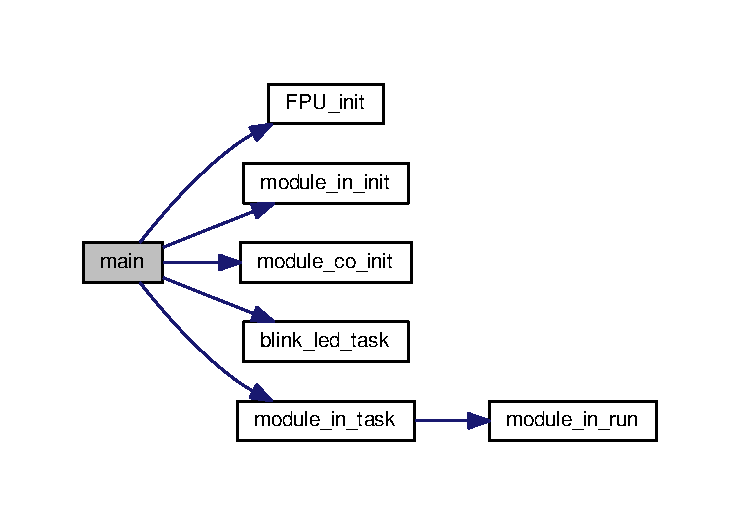
\includegraphics[width=350pt]{group__ProVANT__Modules_ga840291bc02cba5474a4cb46a9b9566fe_cgraph}
\end{center}
\end{figure}


\index{Pro\+V\+A\+N\+T\+\_\+\+Modules@{Pro\+V\+A\+N\+T\+\_\+\+Modules}!module\+\_\+co\+\_\+task@{module\+\_\+co\+\_\+task}}
\index{module\+\_\+co\+\_\+task@{module\+\_\+co\+\_\+task}!Pro\+V\+A\+N\+T\+\_\+\+Modules@{Pro\+V\+A\+N\+T\+\_\+\+Modules}}
\subsubsection[{\texorpdfstring{module\+\_\+co\+\_\+task(void $\ast$pv\+Parameters)}{module_co_task(void *pvParameters)}}]{\setlength{\rightskip}{0pt plus 5cm}void module\+\_\+co\+\_\+task (
\begin{DoxyParamCaption}
\item[{void $\ast$}]{pv\+Parameters}
\end{DoxyParamCaption}
)}\hypertarget{group__ProVANT__Modules_gab0c5d271dba436247302632e599731ba}{}\label{group__ProVANT__Modules_gab0c5d271dba436247302632e599731ba}


Definition at line 115 of file main.\+c.



Here is the call graph for this function\+:\nopagebreak
\begin{figure}[H]
\begin{center}
\leavevmode
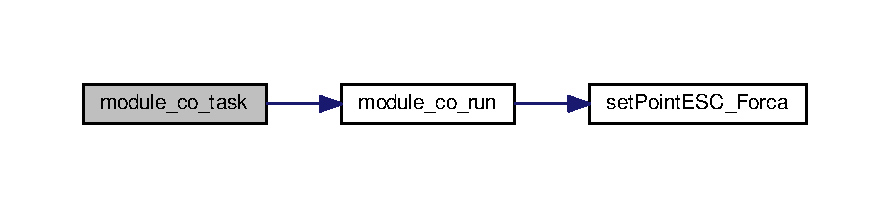
\includegraphics[width=350pt]{group__ProVANT__Modules_gab0c5d271dba436247302632e599731ba_cgraph}
\end{center}
\end{figure}


\index{Pro\+V\+A\+N\+T\+\_\+\+Modules@{Pro\+V\+A\+N\+T\+\_\+\+Modules}!module\+\_\+do\+\_\+task@{module\+\_\+do\+\_\+task}}
\index{module\+\_\+do\+\_\+task@{module\+\_\+do\+\_\+task}!Pro\+V\+A\+N\+T\+\_\+\+Modules@{Pro\+V\+A\+N\+T\+\_\+\+Modules}}
\subsubsection[{\texorpdfstring{module\+\_\+do\+\_\+task(void $\ast$pv\+Parameters)}{module_do_task(void *pvParameters)}}]{\setlength{\rightskip}{0pt plus 5cm}void module\+\_\+do\+\_\+task (
\begin{DoxyParamCaption}
\item[{void $\ast$}]{pv\+Parameters}
\end{DoxyParamCaption}
)}\hypertarget{group__ProVANT__Modules_ga466679da7a6953ce332271681ce397c7}{}\label{group__ProVANT__Modules_ga466679da7a6953ce332271681ce397c7}


Definition at line 127 of file main.\+c.



Here is the call graph for this function\+:\nopagebreak
\begin{figure}[H]
\begin{center}
\leavevmode
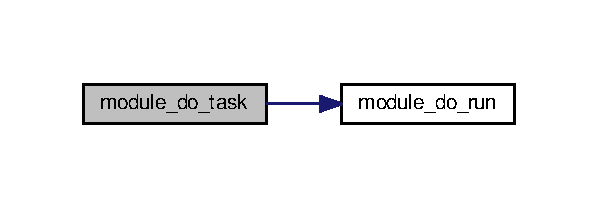
\includegraphics[width=287pt]{group__ProVANT__Modules_ga466679da7a6953ce332271681ce397c7_cgraph}
\end{center}
\end{figure}


\index{Pro\+V\+A\+N\+T\+\_\+\+Modules@{Pro\+V\+A\+N\+T\+\_\+\+Modules}!module\+\_\+gps\+\_\+task@{module\+\_\+gps\+\_\+task}}
\index{module\+\_\+gps\+\_\+task@{module\+\_\+gps\+\_\+task}!Pro\+V\+A\+N\+T\+\_\+\+Modules@{Pro\+V\+A\+N\+T\+\_\+\+Modules}}
\subsubsection[{\texorpdfstring{module\+\_\+gps\+\_\+task(void $\ast$pv\+Parameters)}{module_gps_task(void *pvParameters)}}]{\setlength{\rightskip}{0pt plus 5cm}void module\+\_\+gps\+\_\+task (
\begin{DoxyParamCaption}
\item[{void $\ast$}]{pv\+Parameters}
\end{DoxyParamCaption}
)}\hypertarget{group__ProVANT__Modules_gac55e5b60dffafe957dddc7aa452bfa9d}{}\label{group__ProVANT__Modules_gac55e5b60dffafe957dddc7aa452bfa9d}


Definition at line 133 of file main.\+c.



Here is the call graph for this function\+:\nopagebreak
\begin{figure}[H]
\begin{center}
\leavevmode
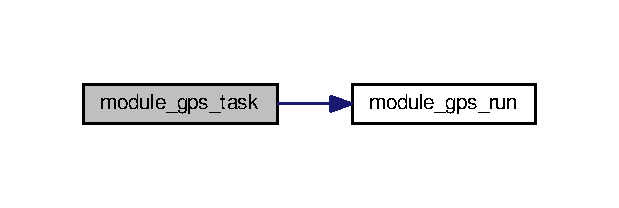
\includegraphics[width=297pt]{group__ProVANT__Modules_gac55e5b60dffafe957dddc7aa452bfa9d_cgraph}
\end{center}
\end{figure}


\index{Pro\+V\+A\+N\+T\+\_\+\+Modules@{Pro\+V\+A\+N\+T\+\_\+\+Modules}!module\+\_\+in\+\_\+task@{module\+\_\+in\+\_\+task}}
\index{module\+\_\+in\+\_\+task@{module\+\_\+in\+\_\+task}!Pro\+V\+A\+N\+T\+\_\+\+Modules@{Pro\+V\+A\+N\+T\+\_\+\+Modules}}
\subsubsection[{\texorpdfstring{module\+\_\+in\+\_\+task(void $\ast$pv\+Parameters)}{module_in_task(void *pvParameters)}}]{\setlength{\rightskip}{0pt plus 5cm}void module\+\_\+in\+\_\+task (
\begin{DoxyParamCaption}
\item[{void $\ast$}]{pv\+Parameters}
\end{DoxyParamCaption}
)}\hypertarget{group__ProVANT__Modules_ga7de15cbee9a0ca9eafb3eb25f5e3d691}{}\label{group__ProVANT__Modules_ga7de15cbee9a0ca9eafb3eb25f5e3d691}


Definition at line 121 of file main.\+c.



Here is the call graph for this function\+:\nopagebreak
\begin{figure}[H]
\begin{center}
\leavevmode
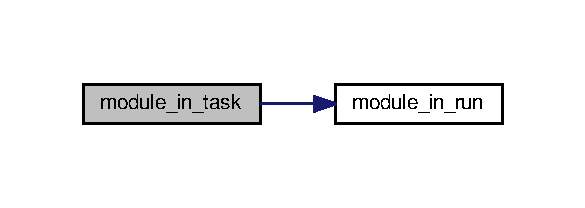
\includegraphics[width=281pt]{group__ProVANT__Modules_ga7de15cbee9a0ca9eafb3eb25f5e3d691_cgraph}
\end{center}
\end{figure}


\index{Pro\+V\+A\+N\+T\+\_\+\+Modules@{Pro\+V\+A\+N\+T\+\_\+\+Modules}!module\+\_\+sm\+\_\+task@{module\+\_\+sm\+\_\+task}}
\index{module\+\_\+sm\+\_\+task@{module\+\_\+sm\+\_\+task}!Pro\+V\+A\+N\+T\+\_\+\+Modules@{Pro\+V\+A\+N\+T\+\_\+\+Modules}}
\subsubsection[{\texorpdfstring{module\+\_\+sm\+\_\+task(void $\ast$pv\+Parameters)}{module_sm_task(void *pvParameters)}}]{\setlength{\rightskip}{0pt plus 5cm}void module\+\_\+sm\+\_\+task (
\begin{DoxyParamCaption}
\item[{void $\ast$}]{pv\+Parameters}
\end{DoxyParamCaption}
)}\hypertarget{group__ProVANT__Modules_gaad8bcaa035ca56eddd3ccbf522298711}{}\label{group__ProVANT__Modules_gaad8bcaa035ca56eddd3ccbf522298711}


Definition at line 139 of file main.\+c.



Here is the call graph for this function\+:\nopagebreak
\begin{figure}[H]
\begin{center}
\leavevmode
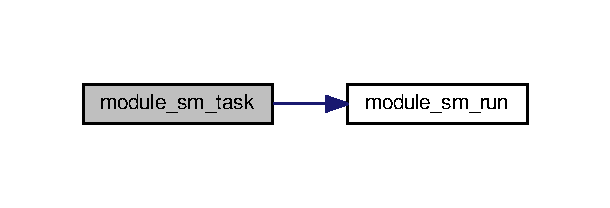
\includegraphics[width=293pt]{group__ProVANT__Modules_gaad8bcaa035ca56eddd3ccbf522298711_cgraph}
\end{center}
\end{figure}


\index{Pro\+V\+A\+N\+T\+\_\+\+Modules@{Pro\+V\+A\+N\+T\+\_\+\+Modules}!v\+Application\+Idle\+Hook@{v\+Application\+Idle\+Hook}}
\index{v\+Application\+Idle\+Hook@{v\+Application\+Idle\+Hook}!Pro\+V\+A\+N\+T\+\_\+\+Modules@{Pro\+V\+A\+N\+T\+\_\+\+Modules}}
\subsubsection[{\texorpdfstring{v\+Application\+Idle\+Hook()}{vApplicationIdleHook()}}]{\setlength{\rightskip}{0pt plus 5cm}void v\+Application\+Idle\+Hook (
\begin{DoxyParamCaption}
{}
\end{DoxyParamCaption}
)}\hypertarget{group__ProVANT__Modules_ga11cbdd335da884dec1204e230554bfd9}{}\label{group__ProVANT__Modules_ga11cbdd335da884dec1204e230554bfd9}


Definition at line 73 of file main.\+c.

\index{Pro\+V\+A\+N\+T\+\_\+\+Modules@{Pro\+V\+A\+N\+T\+\_\+\+Modules}!v\+Application\+Malloc\+Failed\+Hook@{v\+Application\+Malloc\+Failed\+Hook}}
\index{v\+Application\+Malloc\+Failed\+Hook@{v\+Application\+Malloc\+Failed\+Hook}!Pro\+V\+A\+N\+T\+\_\+\+Modules@{Pro\+V\+A\+N\+T\+\_\+\+Modules}}
\subsubsection[{\texorpdfstring{v\+Application\+Malloc\+Failed\+Hook()}{vApplicationMallocFailedHook()}}]{\setlength{\rightskip}{0pt plus 5cm}void v\+Application\+Malloc\+Failed\+Hook (
\begin{DoxyParamCaption}
{}
\end{DoxyParamCaption}
)}\hypertarget{group__ProVANT__Modules_ga73f6aa45470ada02a5d6f3a522d8f13c}{}\label{group__ProVANT__Modules_ga73f6aa45470ada02a5d6f3a522d8f13c}


Definition at line 75 of file main.\+c.

\index{Pro\+V\+A\+N\+T\+\_\+\+Modules@{Pro\+V\+A\+N\+T\+\_\+\+Modules}!v\+Application\+Stack\+Overflow\+Hook@{v\+Application\+Stack\+Overflow\+Hook}}
\index{v\+Application\+Stack\+Overflow\+Hook@{v\+Application\+Stack\+Overflow\+Hook}!Pro\+V\+A\+N\+T\+\_\+\+Modules@{Pro\+V\+A\+N\+T\+\_\+\+Modules}}
\subsubsection[{\texorpdfstring{v\+Application\+Stack\+Overflow\+Hook()}{vApplicationStackOverflowHook()}}]{\setlength{\rightskip}{0pt plus 5cm}void v\+Application\+Stack\+Overflow\+Hook (
\begin{DoxyParamCaption}
{}
\end{DoxyParamCaption}
)}\hypertarget{group__ProVANT__Modules_ga8f5b98d87cfd1379b8d6573159bcbdd3}{}\label{group__ProVANT__Modules_ga8f5b98d87cfd1379b8d6573159bcbdd3}


Definition at line 74 of file main.\+c.

\index{Pro\+V\+A\+N\+T\+\_\+\+Modules@{Pro\+V\+A\+N\+T\+\_\+\+Modules}!v\+Application\+Tick\+Hook@{v\+Application\+Tick\+Hook}}
\index{v\+Application\+Tick\+Hook@{v\+Application\+Tick\+Hook}!Pro\+V\+A\+N\+T\+\_\+\+Modules@{Pro\+V\+A\+N\+T\+\_\+\+Modules}}
\subsubsection[{\texorpdfstring{v\+Application\+Tick\+Hook()}{vApplicationTickHook()}}]{\setlength{\rightskip}{0pt plus 5cm}void v\+Application\+Tick\+Hook (
\begin{DoxyParamCaption}
{}
\end{DoxyParamCaption}
)}\hypertarget{group__ProVANT__Modules_ga2850b09d1bb227364b5ff6de6f85f740}{}\label{group__ProVANT__Modules_ga2850b09d1bb227364b5ff6de6f85f740}


Definition at line 72 of file main.\+c.


\hypertarget{group__ProVANT__app}{}\section{Pro\+V\+A\+N\+T\+\_\+app}
\label{group__ProVANT__app}\index{Pro\+V\+A\+N\+T\+\_\+app@{Pro\+V\+A\+N\+T\+\_\+app}}
Collaboration diagram for Pro\+V\+A\+N\+T\+\_\+app\+:\nopagebreak
\begin{figure}[H]
\begin{center}
\leavevmode
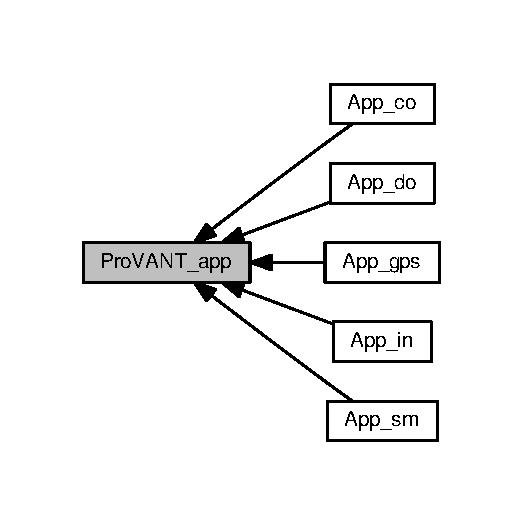
\includegraphics[width=251pt]{group__ProVANT__app}
\end{center}
\end{figure}
\subsection*{Modules}
\begin{DoxyCompactItemize}
\item 
\hyperlink{group__app__co}{App\+\_\+co}
\begin{DoxyCompactList}\small\item\em Módulo com as principais funcionalidades para calculo de controle e escrita de atuadores. \end{DoxyCompactList}\item 
\hyperlink{group__app__do}{App\+\_\+do}
\begin{DoxyCompactList}\small\item\em Módulo responsavel por transmitir dados. \end{DoxyCompactList}\item 
\hyperlink{group__app__gps}{App\+\_\+gps}
\begin{DoxyCompactList}\small\item\em Módulo responsavel por tratar os dados do G\+PS. \end{DoxyCompactList}\item 
\hyperlink{group__app__in}{App\+\_\+in}
\begin{DoxyCompactList}\small\item\em Componentes para o sensoriamento do V\+A\+NT. \end{DoxyCompactList}\item 
\hyperlink{group__app__sm}{App\+\_\+sm}
\begin{DoxyCompactList}\small\item\em Módulo responsavel pela maquina de estados do V\+A\+NT. \end{DoxyCompactList}\end{DoxyCompactItemize}


\subsection{Detailed Description}

\hypertarget{group__app__co}{}\section{App\+\_\+co}
\label{group__app__co}\index{App\+\_\+co@{App\+\_\+co}}


Módulo com as principais funcionalidades para calculo de controle e escrita de atuadores.  


Collaboration diagram for App\+\_\+co\+:\nopagebreak
\begin{figure}[H]
\begin{center}
\leavevmode
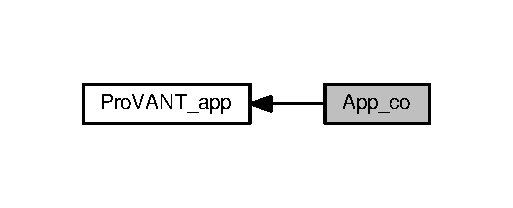
\includegraphics[width=246pt]{group__app__co}
\end{center}
\end{figure}
\subsection*{Macros}
\begin{DoxyCompactItemize}
\item 
\#define \hyperlink{group__app__co_ga0ac6c9f2991b096e49c354e5cce6fae0}{M\+O\+D\+U\+L\+E\+\_\+\+P\+E\+R\+I\+OD}~12
\item 
\#define \hyperlink{group__app__co_gaec8246e954743c1eca3ed9d0b934bf8e}{E\+S\+C\+\_\+\+ON}~1
\item 
\#define \hyperlink{group__app__co_ga162e9e4abd94f1558733bbf17fca28e9}{S\+E\+R\+V\+O\+\_\+\+ON}~1
\item 
\#define \hyperlink{group__app__co_ga6a53a6c94a70cc286e300a0ea8f46ba4}{U\+S\+A\+R\+T\+\_\+\+B\+A\+U\+D\+R\+A\+TE}~921600
\end{DoxyCompactItemize}
\subsection*{Functions}
\begin{DoxyCompactItemize}
\item 
unsigned char \hyperlink{group__app__co_gac9b9b4433da08cf375a9089fbb464b74}{set\+Point\+E\+S\+C\+\_\+\+Forca} (float forca)
\item 
void \hyperlink{group__app__co_gabedb9a5c3739466a359c93b3585a3640}{module\+\_\+co\+\_\+init} ()
\begin{DoxyCompactList}\small\item\em Inicializacao do módulo de controle + output. \end{DoxyCompactList}\item 
void \hyperlink{group__app__co_gaab8216fc955d01b47e3431aae288d9d3}{module\+\_\+co\+\_\+run} ()
\begin{DoxyCompactList}\small\item\em Função principal do módulo de RC. \end{DoxyCompactList}\end{DoxyCompactItemize}
\subsection*{Variables}
\begin{DoxyCompactItemize}
\item 
port\+Tick\+Type \hyperlink{group__app__co_gab06dc9c7b584f053bcde9e3dd366c886}{pv\+\_\+module\+\_\+co\+\_\+last\+Wake\+Time}
\item 
pv\+\_\+msg\+\_\+input \hyperlink{group__app__co_gac40b8cfe5fd2000670ad57fe3e75ec89}{i\+Input\+Data}
\item 
pv\+\_\+msg\+\_\+control\+Output \hyperlink{group__app__co_ga01528088e36182dce9f2d7126db89886}{i\+Control\+Beagle\+Data}
\item 
pv\+\_\+msg\+\_\+control\+Output \hyperlink{group__app__co_ga0a14ca4568444d2d76c256fa91585cdf}{o\+Control\+Output\+Data}
\item 
pv\+\_\+type\+\_\+actuation \hyperlink{group__app__co_gaf0fb0cf3bcfc492356d3cbe85376efa3}{pv\+\_\+module\+\_\+co\+\_\+actuation}
\item 
int \hyperlink{group__app__co_ga4e39239e9a359dfd174056754a046b8a}{pv\+\_\+module\+\_\+co\+\_\+flag}
\item 
G\+P\+I\+O\+Pin \hyperlink{group__app__co_gaa7d4da6aed3ca0087db45a3706ef17fa}{pv\+\_\+module\+\_\+co\+\_\+\+L\+E\+D5}
\item 
pv\+\_\+type\+\_\+actuation \hyperlink{group__app__co_gaf6cc28f22186e2338a688b8e76d8c975}{i\+Actuation}
\end{DoxyCompactItemize}


\subsection{Detailed Description}
Módulo com as principais funcionalidades para calculo de controle e escrita de atuadores. 

Definição do módulo. 

\subsection{Macro Definition Documentation}
\index{App\+\_\+co@{App\+\_\+co}!E\+S\+C\+\_\+\+ON@{E\+S\+C\+\_\+\+ON}}
\index{E\+S\+C\+\_\+\+ON@{E\+S\+C\+\_\+\+ON}!App\+\_\+co@{App\+\_\+co}}
\subsubsection[{\texorpdfstring{E\+S\+C\+\_\+\+ON}{ESC_ON}}]{\setlength{\rightskip}{0pt plus 5cm}\#define E\+S\+C\+\_\+\+ON~1}\hypertarget{group__app__co_gaec8246e954743c1eca3ed9d0b934bf8e}{}\label{group__app__co_gaec8246e954743c1eca3ed9d0b934bf8e}


Definition at line 27 of file pv\+\_\+module\+\_\+co.\+c.

\index{App\+\_\+co@{App\+\_\+co}!M\+O\+D\+U\+L\+E\+\_\+\+P\+E\+R\+I\+OD@{M\+O\+D\+U\+L\+E\+\_\+\+P\+E\+R\+I\+OD}}
\index{M\+O\+D\+U\+L\+E\+\_\+\+P\+E\+R\+I\+OD@{M\+O\+D\+U\+L\+E\+\_\+\+P\+E\+R\+I\+OD}!App\+\_\+co@{App\+\_\+co}}
\subsubsection[{\texorpdfstring{M\+O\+D\+U\+L\+E\+\_\+\+P\+E\+R\+I\+OD}{MODULE_PERIOD}}]{\setlength{\rightskip}{0pt plus 5cm}\#define M\+O\+D\+U\+L\+E\+\_\+\+P\+E\+R\+I\+OD~12}\hypertarget{group__app__co_ga0ac6c9f2991b096e49c354e5cce6fae0}{}\label{group__app__co_ga0ac6c9f2991b096e49c354e5cce6fae0}


Definition at line 26 of file pv\+\_\+module\+\_\+co.\+c.

\index{App\+\_\+co@{App\+\_\+co}!S\+E\+R\+V\+O\+\_\+\+ON@{S\+E\+R\+V\+O\+\_\+\+ON}}
\index{S\+E\+R\+V\+O\+\_\+\+ON@{S\+E\+R\+V\+O\+\_\+\+ON}!App\+\_\+co@{App\+\_\+co}}
\subsubsection[{\texorpdfstring{S\+E\+R\+V\+O\+\_\+\+ON}{SERVO_ON}}]{\setlength{\rightskip}{0pt plus 5cm}\#define S\+E\+R\+V\+O\+\_\+\+ON~1}\hypertarget{group__app__co_ga162e9e4abd94f1558733bbf17fca28e9}{}\label{group__app__co_ga162e9e4abd94f1558733bbf17fca28e9}


Definition at line 28 of file pv\+\_\+module\+\_\+co.\+c.

\index{App\+\_\+co@{App\+\_\+co}!U\+S\+A\+R\+T\+\_\+\+B\+A\+U\+D\+R\+A\+TE@{U\+S\+A\+R\+T\+\_\+\+B\+A\+U\+D\+R\+A\+TE}}
\index{U\+S\+A\+R\+T\+\_\+\+B\+A\+U\+D\+R\+A\+TE@{U\+S\+A\+R\+T\+\_\+\+B\+A\+U\+D\+R\+A\+TE}!App\+\_\+co@{App\+\_\+co}}
\subsubsection[{\texorpdfstring{U\+S\+A\+R\+T\+\_\+\+B\+A\+U\+D\+R\+A\+TE}{USART_BAUDRATE}}]{\setlength{\rightskip}{0pt plus 5cm}\#define U\+S\+A\+R\+T\+\_\+\+B\+A\+U\+D\+R\+A\+TE~921600}\hypertarget{group__app__co_ga6a53a6c94a70cc286e300a0ea8f46ba4}{}\label{group__app__co_ga6a53a6c94a70cc286e300a0ea8f46ba4}


Definition at line 31 of file pv\+\_\+module\+\_\+co.\+c.



\subsection{Function Documentation}
\index{App\+\_\+co@{App\+\_\+co}!module\+\_\+co\+\_\+init@{module\+\_\+co\+\_\+init}}
\index{module\+\_\+co\+\_\+init@{module\+\_\+co\+\_\+init}!App\+\_\+co@{App\+\_\+co}}
\subsubsection[{\texorpdfstring{module\+\_\+co\+\_\+init()}{module_co_init()}}]{\setlength{\rightskip}{0pt plus 5cm}void module\+\_\+co\+\_\+init (
\begin{DoxyParamCaption}
{}
\end{DoxyParamCaption}
)}\hypertarget{group__app__co_gabedb9a5c3739466a359c93b3585a3640}{}\label{group__app__co_gabedb9a5c3739466a359c93b3585a3640}


Inicializacao do módulo de controle + output. 

Instancia as Queues de comunicação inter-\/thread, inicializa a pinagem necessária para os perifericos e aloca o que for necessário para as equações de controle. 
\begin{DoxyParams}{Parameters}
{\em None} & \\
\hline
\end{DoxyParams}

\begin{DoxyRetVals}{Return values}
{\em None} & \\
\hline
\end{DoxyRetVals}


Definition at line 57 of file pv\+\_\+module\+\_\+co.\+c.

\index{App\+\_\+co@{App\+\_\+co}!module\+\_\+co\+\_\+run@{module\+\_\+co\+\_\+run}}
\index{module\+\_\+co\+\_\+run@{module\+\_\+co\+\_\+run}!App\+\_\+co@{App\+\_\+co}}
\subsubsection[{\texorpdfstring{module\+\_\+co\+\_\+run()}{module_co_run()}}]{\setlength{\rightskip}{0pt plus 5cm}void module\+\_\+co\+\_\+run (
\begin{DoxyParamCaption}
{}
\end{DoxyParamCaption}
)}\hypertarget{group__app__co_gaab8216fc955d01b47e3431aae288d9d3}{}\label{group__app__co_gaab8216fc955d01b47e3431aae288d9d3}


Função principal do módulo de RC. 


\begin{DoxyParams}{Parameters}
{\em None} & \\
\hline
\end{DoxyParams}

\begin{DoxyRetVals}{Return values}
{\em None} & Interpreta o recebimento de P\+PM, calcula sinais de controle e os envia via interface. Devido as diferenças do modelo matematica com a construção mecanica o sinal do angulo do servo direito deve ser adaptado. \\
\hline
\end{DoxyRetVals}


Definition at line 92 of file pv\+\_\+module\+\_\+co.\+c.



Here is the call graph for this function\+:\nopagebreak
\begin{figure}[H]
\begin{center}
\leavevmode
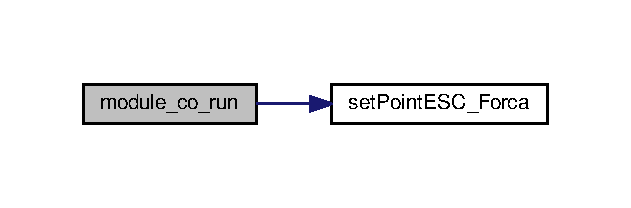
\includegraphics[width=303pt]{group__app__co_gaab8216fc955d01b47e3431aae288d9d3_cgraph}
\end{center}
\end{figure}


\index{App\+\_\+co@{App\+\_\+co}!set\+Point\+E\+S\+C\+\_\+\+Forca@{set\+Point\+E\+S\+C\+\_\+\+Forca}}
\index{set\+Point\+E\+S\+C\+\_\+\+Forca@{set\+Point\+E\+S\+C\+\_\+\+Forca}!App\+\_\+co@{App\+\_\+co}}
\subsubsection[{\texorpdfstring{set\+Point\+E\+S\+C\+\_\+\+Forca(float forca)}{setPointESC_Forca(float forca)}}]{\setlength{\rightskip}{0pt plus 5cm}unsigned char set\+Point\+E\+S\+C\+\_\+\+Forca (
\begin{DoxyParamCaption}
\item[{float}]{forca}
\end{DoxyParamCaption}
)}\hypertarget{group__app__co_gac9b9b4433da08cf375a9089fbb464b74}{}\label{group__app__co_gac9b9b4433da08cf375a9089fbb464b74}
\textbackslash{} brief Calcula o set point do E\+SC a partir da forca passada por argumento Curva retirada dos ensaios com os motores brushless no I\+N\+EP 

Definition at line 288 of file pv\+\_\+module\+\_\+co.\+c.



\subsection{Variable Documentation}
\index{App\+\_\+co@{App\+\_\+co}!i\+Actuation@{i\+Actuation}}
\index{i\+Actuation@{i\+Actuation}!App\+\_\+co@{App\+\_\+co}}
\subsubsection[{\texorpdfstring{i\+Actuation}{iActuation}}]{\setlength{\rightskip}{0pt plus 5cm}pv\+\_\+type\+\_\+actuation i\+Actuation}\hypertarget{group__app__co_gaf6cc28f22186e2338a688b8e76d8c975}{}\label{group__app__co_gaf6cc28f22186e2338a688b8e76d8c975}


Definition at line 42 of file pv\+\_\+module\+\_\+co.\+c.

\index{App\+\_\+co@{App\+\_\+co}!i\+Control\+Beagle\+Data@{i\+Control\+Beagle\+Data}}
\index{i\+Control\+Beagle\+Data@{i\+Control\+Beagle\+Data}!App\+\_\+co@{App\+\_\+co}}
\subsubsection[{\texorpdfstring{i\+Control\+Beagle\+Data}{iControlBeagleData}}]{\setlength{\rightskip}{0pt plus 5cm}pv\+\_\+msg\+\_\+control\+Output i\+Control\+Beagle\+Data}\hypertarget{group__app__co_ga01528088e36182dce9f2d7126db89886}{}\label{group__app__co_ga01528088e36182dce9f2d7126db89886}


Definition at line 35 of file pv\+\_\+module\+\_\+co.\+c.

\index{App\+\_\+co@{App\+\_\+co}!i\+Input\+Data@{i\+Input\+Data}}
\index{i\+Input\+Data@{i\+Input\+Data}!App\+\_\+co@{App\+\_\+co}}
\subsubsection[{\texorpdfstring{i\+Input\+Data}{iInputData}}]{\setlength{\rightskip}{0pt plus 5cm}pv\+\_\+msg\+\_\+input i\+Input\+Data}\hypertarget{group__app__co_gac40b8cfe5fd2000670ad57fe3e75ec89}{}\label{group__app__co_gac40b8cfe5fd2000670ad57fe3e75ec89}


Definition at line 34 of file pv\+\_\+module\+\_\+co.\+c.

\index{App\+\_\+co@{App\+\_\+co}!o\+Control\+Output\+Data@{o\+Control\+Output\+Data}}
\index{o\+Control\+Output\+Data@{o\+Control\+Output\+Data}!App\+\_\+co@{App\+\_\+co}}
\subsubsection[{\texorpdfstring{o\+Control\+Output\+Data}{oControlOutputData}}]{\setlength{\rightskip}{0pt plus 5cm}pv\+\_\+msg\+\_\+control\+Output o\+Control\+Output\+Data}\hypertarget{group__app__co_ga0a14ca4568444d2d76c256fa91585cdf}{}\label{group__app__co_ga0a14ca4568444d2d76c256fa91585cdf}


Definition at line 36 of file pv\+\_\+module\+\_\+co.\+c.

\index{App\+\_\+co@{App\+\_\+co}!pv\+\_\+module\+\_\+co\+\_\+actuation@{pv\+\_\+module\+\_\+co\+\_\+actuation}}
\index{pv\+\_\+module\+\_\+co\+\_\+actuation@{pv\+\_\+module\+\_\+co\+\_\+actuation}!App\+\_\+co@{App\+\_\+co}}
\subsubsection[{\texorpdfstring{pv\+\_\+module\+\_\+co\+\_\+actuation}{pv_module_co_actuation}}]{\setlength{\rightskip}{0pt plus 5cm}pv\+\_\+type\+\_\+actuation pv\+\_\+module\+\_\+co\+\_\+actuation}\hypertarget{group__app__co_gaf0fb0cf3bcfc492356d3cbe85376efa3}{}\label{group__app__co_gaf0fb0cf3bcfc492356d3cbe85376efa3}


Definition at line 37 of file pv\+\_\+module\+\_\+co.\+c.

\index{App\+\_\+co@{App\+\_\+co}!pv\+\_\+module\+\_\+co\+\_\+flag@{pv\+\_\+module\+\_\+co\+\_\+flag}}
\index{pv\+\_\+module\+\_\+co\+\_\+flag@{pv\+\_\+module\+\_\+co\+\_\+flag}!App\+\_\+co@{App\+\_\+co}}
\subsubsection[{\texorpdfstring{pv\+\_\+module\+\_\+co\+\_\+flag}{pv_module_co_flag}}]{\setlength{\rightskip}{0pt plus 5cm}int pv\+\_\+module\+\_\+co\+\_\+flag}\hypertarget{group__app__co_ga4e39239e9a359dfd174056754a046b8a}{}\label{group__app__co_ga4e39239e9a359dfd174056754a046b8a}


Definition at line 38 of file pv\+\_\+module\+\_\+co.\+c.

\index{App\+\_\+co@{App\+\_\+co}!pv\+\_\+module\+\_\+co\+\_\+last\+Wake\+Time@{pv\+\_\+module\+\_\+co\+\_\+last\+Wake\+Time}}
\index{pv\+\_\+module\+\_\+co\+\_\+last\+Wake\+Time@{pv\+\_\+module\+\_\+co\+\_\+last\+Wake\+Time}!App\+\_\+co@{App\+\_\+co}}
\subsubsection[{\texorpdfstring{pv\+\_\+module\+\_\+co\+\_\+last\+Wake\+Time}{pv_module_co_lastWakeTime}}]{\setlength{\rightskip}{0pt plus 5cm}port\+Tick\+Type pv\+\_\+module\+\_\+co\+\_\+last\+Wake\+Time}\hypertarget{group__app__co_gab06dc9c7b584f053bcde9e3dd366c886}{}\label{group__app__co_gab06dc9c7b584f053bcde9e3dd366c886}


Definition at line 33 of file pv\+\_\+module\+\_\+co.\+c.

\index{App\+\_\+co@{App\+\_\+co}!pv\+\_\+module\+\_\+co\+\_\+\+L\+E\+D5@{pv\+\_\+module\+\_\+co\+\_\+\+L\+E\+D5}}
\index{pv\+\_\+module\+\_\+co\+\_\+\+L\+E\+D5@{pv\+\_\+module\+\_\+co\+\_\+\+L\+E\+D5}!App\+\_\+co@{App\+\_\+co}}
\subsubsection[{\texorpdfstring{pv\+\_\+module\+\_\+co\+\_\+\+L\+E\+D5}{pv_module_co_LED5}}]{\setlength{\rightskip}{0pt plus 5cm}G\+P\+I\+O\+Pin pv\+\_\+module\+\_\+co\+\_\+\+L\+E\+D5}\hypertarget{group__app__co_gaa7d4da6aed3ca0087db45a3706ef17fa}{}\label{group__app__co_gaa7d4da6aed3ca0087db45a3706ef17fa}


Definition at line 39 of file pv\+\_\+module\+\_\+co.\+c.


\hypertarget{group__app__do}{}\section{App\+\_\+do}
\label{group__app__do}\index{App\+\_\+do@{App\+\_\+do}}


Módulo responsavel por transmitir dados.  


Collaboration diagram for App\+\_\+do\+:\nopagebreak
\begin{figure}[H]
\begin{center}
\leavevmode
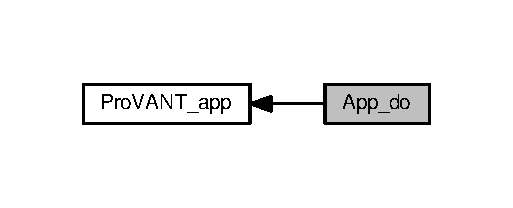
\includegraphics[width=246pt]{group__app__do}
\end{center}
\end{figure}
\subsection*{Macros}
\begin{DoxyCompactItemize}
\item 
\#define \hyperlink{group__app__do_ga0ac6c9f2991b096e49c354e5cce6fae0}{M\+O\+D\+U\+L\+E\+\_\+\+P\+E\+R\+I\+OD}~15
\item 
\#define \hyperlink{group__app__do_ga6a53a6c94a70cc286e300a0ea8f46ba4}{U\+S\+A\+R\+T\+\_\+\+B\+A\+U\+D\+R\+A\+TE}~921600
\end{DoxyCompactItemize}
\subsection*{Functions}
\begin{DoxyCompactItemize}
\item 
void \hyperlink{group__app__do_ga901c023651503207f5cfd8cdb8c305b3}{module\+\_\+do\+\_\+init} ()
\begin{DoxyCompactList}\small\item\em Inicializacao do módulo de data out. \end{DoxyCompactList}\item 
void \hyperlink{group__app__do_ga1f08b4b431624465a47f47eca0520253}{module\+\_\+do\+\_\+run} ()
\begin{DoxyCompactList}\small\item\em Função principal do módulo de data out. \end{DoxyCompactList}\end{DoxyCompactItemize}
\subsection*{Variables}
\begin{DoxyCompactItemize}
\item 
port\+Tick\+Type \hyperlink{group__app__do_gaa8db3871cb5f64abbd94ddd5a1db73a6}{last\+Wake\+Time}
\item 
unsigned int \hyperlink{group__app__do_ga24475be702ffcc5a6f0a5557040368ef}{heart\+Beat} =0
\item 
unsigned int \hyperlink{group__app__do_ga5bdb7b29978109a480db66886e58f475}{cicle\+Time} =0
\item 
pv\+\_\+msg\+\_\+input \hyperlink{group__app__do_gac40b8cfe5fd2000670ad57fe3e75ec89}{i\+Input\+Data}
\item 
pv\+\_\+msg\+\_\+gps \hyperlink{group__app__do_gac433f205128f94bd944f8ddcbff92744}{i\+Gps\+Data}
\item 
pv\+\_\+msg\+\_\+control\+Output \hyperlink{group__app__do_gacabca53fbaffdbf13b8e5a1c29b73bc4}{i\+Control\+Output\+Data}
\item 
pv\+\_\+msg\+\_\+control\+Output \hyperlink{group__app__do_ga83a7ee8a519c421eec8b1c7efc9e0501}{o\+Control\+Beagle\+Data}
\item 
float \hyperlink{group__app__do_ga1ba0a7c98794a4cda502c52d222ab614}{rpy} \mbox{[}3\mbox{]}
\item 
float \hyperlink{group__app__do_ga09c67ab670708cf621c9853aeb34fc2c}{drpy} \mbox{[}3\mbox{]}
\item 
float \hyperlink{group__app__do_ga1a3ca0a0bf0cdb13a8689c0558ead4df}{position} \mbox{[}3\mbox{]}
\item 
float \hyperlink{group__app__do_ga63a3bb0717d926f2f94b982b96e92237}{velocity} \mbox{[}3\mbox{]}
\item 
float \hyperlink{group__app__do_gaf2c21f3aed6186d912908dcd33a057d6}{alpha} \mbox{[}2\mbox{]}
\item 
float \hyperlink{group__app__do_gac55455b51b6abc065db2bfa3a99c0783}{dalpha} \mbox{[}2\mbox{]}
\item 
float \hyperlink{group__app__do_ga44b306459efc6e5e3543390e98fa8df7}{data1} \mbox{[}2\mbox{]}
\item 
float \hyperlink{group__app__do_ga2241fa8ef7e6a940cd8ce8dc13d8b4e8}{data2} \mbox{[}2\mbox{]}
\item 
float \hyperlink{group__app__do_gafb91c0f3a7dabe2beb8c046ff3cd4613}{data3} \mbox{[}2\mbox{]}
\item 
int \hyperlink{group__app__do_ga5acd447dc75f4ac13cdac246a2c75291}{aux} \mbox{[}2\mbox{]}
\item 
float \hyperlink{group__app__do_gae93eafaee31c92a65f90bcb26eda96df}{aux2} \mbox{[}3\mbox{]}
\item 
float \hyperlink{group__app__do_gaa56fed06b51b312e13aa20c0c740795e}{servo\+Torque} \mbox{[}2\mbox{]}
\item 
float \hyperlink{group__app__do_ga7b919fc59fbb86e34627c65320446dd3}{esc\+Force} \mbox{[}2\mbox{]}
\item 
int \hyperlink{group__app__do_ga7738565d91833be3229136a1beaaf44b}{channel} \mbox{[}7\mbox{]}
\item 
G\+P\+I\+O\+Pin \hyperlink{group__app__do_ga804d3aba22a782022afc3977966f2faa}{L\+E\+D3}
\end{DoxyCompactItemize}


\subsection{Detailed Description}
Módulo responsavel por transmitir dados. 

Definição do módulo de transmissão de dados. 

\subsection{Macro Definition Documentation}
\index{App\+\_\+do@{App\+\_\+do}!M\+O\+D\+U\+L\+E\+\_\+\+P\+E\+R\+I\+OD@{M\+O\+D\+U\+L\+E\+\_\+\+P\+E\+R\+I\+OD}}
\index{M\+O\+D\+U\+L\+E\+\_\+\+P\+E\+R\+I\+OD@{M\+O\+D\+U\+L\+E\+\_\+\+P\+E\+R\+I\+OD}!App\+\_\+do@{App\+\_\+do}}
\subsubsection[{\texorpdfstring{M\+O\+D\+U\+L\+E\+\_\+\+P\+E\+R\+I\+OD}{MODULE_PERIOD}}]{\setlength{\rightskip}{0pt plus 5cm}\#define M\+O\+D\+U\+L\+E\+\_\+\+P\+E\+R\+I\+OD~15}\hypertarget{group__app__do_ga0ac6c9f2991b096e49c354e5cce6fae0}{}\label{group__app__do_ga0ac6c9f2991b096e49c354e5cce6fae0}


Definition at line 26 of file pv\+\_\+module\+\_\+do.\+c.

\index{App\+\_\+do@{App\+\_\+do}!U\+S\+A\+R\+T\+\_\+\+B\+A\+U\+D\+R\+A\+TE@{U\+S\+A\+R\+T\+\_\+\+B\+A\+U\+D\+R\+A\+TE}}
\index{U\+S\+A\+R\+T\+\_\+\+B\+A\+U\+D\+R\+A\+TE@{U\+S\+A\+R\+T\+\_\+\+B\+A\+U\+D\+R\+A\+TE}!App\+\_\+do@{App\+\_\+do}}
\subsubsection[{\texorpdfstring{U\+S\+A\+R\+T\+\_\+\+B\+A\+U\+D\+R\+A\+TE}{USART_BAUDRATE}}]{\setlength{\rightskip}{0pt plus 5cm}\#define U\+S\+A\+R\+T\+\_\+\+B\+A\+U\+D\+R\+A\+TE~921600}\hypertarget{group__app__do_ga6a53a6c94a70cc286e300a0ea8f46ba4}{}\label{group__app__do_ga6a53a6c94a70cc286e300a0ea8f46ba4}


Definition at line 28 of file pv\+\_\+module\+\_\+do.\+c.



\subsection{Function Documentation}
\index{App\+\_\+do@{App\+\_\+do}!module\+\_\+do\+\_\+init@{module\+\_\+do\+\_\+init}}
\index{module\+\_\+do\+\_\+init@{module\+\_\+do\+\_\+init}!App\+\_\+do@{App\+\_\+do}}
\subsubsection[{\texorpdfstring{module\+\_\+do\+\_\+init()}{module_do_init()}}]{\setlength{\rightskip}{0pt plus 5cm}void module\+\_\+do\+\_\+init (
\begin{DoxyParamCaption}
{}
\end{DoxyParamCaption}
)}\hypertarget{group__app__do_ga901c023651503207f5cfd8cdb8c305b3}{}\label{group__app__do_ga901c023651503207f5cfd8cdb8c305b3}


Inicializacao do módulo de data out. 

Instancia as Queues de comunicação inter-\/thread. 
\begin{DoxyParams}{Parameters}
{\em None} & \\
\hline
\end{DoxyParams}

\begin{DoxyRetVals}{Return values}
{\em None} & \\
\hline
\end{DoxyRetVals}


Definition at line 64 of file pv\+\_\+module\+\_\+do.\+c.

\index{App\+\_\+do@{App\+\_\+do}!module\+\_\+do\+\_\+run@{module\+\_\+do\+\_\+run}}
\index{module\+\_\+do\+\_\+run@{module\+\_\+do\+\_\+run}!App\+\_\+do@{App\+\_\+do}}
\subsubsection[{\texorpdfstring{module\+\_\+do\+\_\+run()}{module_do_run()}}]{\setlength{\rightskip}{0pt plus 5cm}void module\+\_\+do\+\_\+run (
\begin{DoxyParamCaption}
{}
\end{DoxyParamCaption}
)}\hypertarget{group__app__do_ga1f08b4b431624465a47f47eca0520253}{}\label{group__app__do_ga1f08b4b431624465a47f47eca0520253}


Função principal do módulo de data out. 


\begin{DoxyParams}{Parameters}
{\em None} & \\
\hline
\end{DoxyParams}

\begin{DoxyRetVals}{Return values}
{\em None} & \\
\hline
\end{DoxyRetVals}


Definition at line 87 of file pv\+\_\+module\+\_\+do.\+c.



\subsection{Variable Documentation}
\index{App\+\_\+do@{App\+\_\+do}!alpha@{alpha}}
\index{alpha@{alpha}!App\+\_\+do@{App\+\_\+do}}
\subsubsection[{\texorpdfstring{alpha}{alpha}}]{\setlength{\rightskip}{0pt plus 5cm}float alpha\mbox{[}2\mbox{]}}\hypertarget{group__app__do_gaf2c21f3aed6186d912908dcd33a057d6}{}\label{group__app__do_gaf2c21f3aed6186d912908dcd33a057d6}


Definition at line 44 of file pv\+\_\+module\+\_\+do.\+c.

\index{App\+\_\+do@{App\+\_\+do}!aux@{aux}}
\index{aux@{aux}!App\+\_\+do@{App\+\_\+do}}
\subsubsection[{\texorpdfstring{aux}{aux}}]{\setlength{\rightskip}{0pt plus 5cm}int aux\mbox{[}2\mbox{]}}\hypertarget{group__app__do_ga5acd447dc75f4ac13cdac246a2c75291}{}\label{group__app__do_ga5acd447dc75f4ac13cdac246a2c75291}


Definition at line 47 of file pv\+\_\+module\+\_\+do.\+c.

\index{App\+\_\+do@{App\+\_\+do}!aux2@{aux2}}
\index{aux2@{aux2}!App\+\_\+do@{App\+\_\+do}}
\subsubsection[{\texorpdfstring{aux2}{aux2}}]{\setlength{\rightskip}{0pt plus 5cm}float aux2\mbox{[}3\mbox{]}}\hypertarget{group__app__do_gae93eafaee31c92a65f90bcb26eda96df}{}\label{group__app__do_gae93eafaee31c92a65f90bcb26eda96df}


Definition at line 48 of file pv\+\_\+module\+\_\+do.\+c.

\index{App\+\_\+do@{App\+\_\+do}!channel@{channel}}
\index{channel@{channel}!App\+\_\+do@{App\+\_\+do}}
\subsubsection[{\texorpdfstring{channel}{channel}}]{\setlength{\rightskip}{0pt plus 5cm}int channel\mbox{[}7\mbox{]}}\hypertarget{group__app__do_ga7738565d91833be3229136a1beaaf44b}{}\label{group__app__do_ga7738565d91833be3229136a1beaaf44b}


Definition at line 51 of file pv\+\_\+module\+\_\+do.\+c.

\index{App\+\_\+do@{App\+\_\+do}!cicle\+Time@{cicle\+Time}}
\index{cicle\+Time@{cicle\+Time}!App\+\_\+do@{App\+\_\+do}}
\subsubsection[{\texorpdfstring{cicle\+Time}{cicleTime}}]{\setlength{\rightskip}{0pt plus 5cm}unsigned int cicle\+Time =0}\hypertarget{group__app__do_ga5bdb7b29978109a480db66886e58f475}{}\label{group__app__do_ga5bdb7b29978109a480db66886e58f475}


Definition at line 35 of file pv\+\_\+module\+\_\+do.\+c.

\index{App\+\_\+do@{App\+\_\+do}!dalpha@{dalpha}}
\index{dalpha@{dalpha}!App\+\_\+do@{App\+\_\+do}}
\subsubsection[{\texorpdfstring{dalpha}{dalpha}}]{\setlength{\rightskip}{0pt plus 5cm}float dalpha\mbox{[}2\mbox{]}}\hypertarget{group__app__do_gac55455b51b6abc065db2bfa3a99c0783}{}\label{group__app__do_gac55455b51b6abc065db2bfa3a99c0783}


Definition at line 45 of file pv\+\_\+module\+\_\+do.\+c.

\index{App\+\_\+do@{App\+\_\+do}!data1@{data1}}
\index{data1@{data1}!App\+\_\+do@{App\+\_\+do}}
\subsubsection[{\texorpdfstring{data1}{data1}}]{\setlength{\rightskip}{0pt plus 5cm}float data1\mbox{[}2\mbox{]}}\hypertarget{group__app__do_ga44b306459efc6e5e3543390e98fa8df7}{}\label{group__app__do_ga44b306459efc6e5e3543390e98fa8df7}


Definition at line 46 of file pv\+\_\+module\+\_\+do.\+c.

\index{App\+\_\+do@{App\+\_\+do}!data2@{data2}}
\index{data2@{data2}!App\+\_\+do@{App\+\_\+do}}
\subsubsection[{\texorpdfstring{data2}{data2}}]{\setlength{\rightskip}{0pt plus 5cm}float data2\mbox{[}2\mbox{]}}\hypertarget{group__app__do_ga2241fa8ef7e6a940cd8ce8dc13d8b4e8}{}\label{group__app__do_ga2241fa8ef7e6a940cd8ce8dc13d8b4e8}


Definition at line 46 of file pv\+\_\+module\+\_\+do.\+c.

\index{App\+\_\+do@{App\+\_\+do}!data3@{data3}}
\index{data3@{data3}!App\+\_\+do@{App\+\_\+do}}
\subsubsection[{\texorpdfstring{data3}{data3}}]{\setlength{\rightskip}{0pt plus 5cm}float data3\mbox{[}2\mbox{]}}\hypertarget{group__app__do_gafb91c0f3a7dabe2beb8c046ff3cd4613}{}\label{group__app__do_gafb91c0f3a7dabe2beb8c046ff3cd4613}


Definition at line 46 of file pv\+\_\+module\+\_\+do.\+c.

\index{App\+\_\+do@{App\+\_\+do}!drpy@{drpy}}
\index{drpy@{drpy}!App\+\_\+do@{App\+\_\+do}}
\subsubsection[{\texorpdfstring{drpy}{drpy}}]{\setlength{\rightskip}{0pt plus 5cm}float drpy\mbox{[}3\mbox{]}}\hypertarget{group__app__do_ga09c67ab670708cf621c9853aeb34fc2c}{}\label{group__app__do_ga09c67ab670708cf621c9853aeb34fc2c}


Definition at line 41 of file pv\+\_\+module\+\_\+do.\+c.

\index{App\+\_\+do@{App\+\_\+do}!esc\+Force@{esc\+Force}}
\index{esc\+Force@{esc\+Force}!App\+\_\+do@{App\+\_\+do}}
\subsubsection[{\texorpdfstring{esc\+Force}{escForce}}]{\setlength{\rightskip}{0pt plus 5cm}float esc\+Force\mbox{[}2\mbox{]}}\hypertarget{group__app__do_ga7b919fc59fbb86e34627c65320446dd3}{}\label{group__app__do_ga7b919fc59fbb86e34627c65320446dd3}


Definition at line 50 of file pv\+\_\+module\+\_\+do.\+c.

\index{App\+\_\+do@{App\+\_\+do}!heart\+Beat@{heart\+Beat}}
\index{heart\+Beat@{heart\+Beat}!App\+\_\+do@{App\+\_\+do}}
\subsubsection[{\texorpdfstring{heart\+Beat}{heartBeat}}]{\setlength{\rightskip}{0pt plus 5cm}unsigned int heart\+Beat =0}\hypertarget{group__app__do_ga24475be702ffcc5a6f0a5557040368ef}{}\label{group__app__do_ga24475be702ffcc5a6f0a5557040368ef}


Definition at line 34 of file pv\+\_\+module\+\_\+do.\+c.

\index{App\+\_\+do@{App\+\_\+do}!i\+Control\+Output\+Data@{i\+Control\+Output\+Data}}
\index{i\+Control\+Output\+Data@{i\+Control\+Output\+Data}!App\+\_\+do@{App\+\_\+do}}
\subsubsection[{\texorpdfstring{i\+Control\+Output\+Data}{iControlOutputData}}]{\setlength{\rightskip}{0pt plus 5cm}pv\+\_\+msg\+\_\+control\+Output i\+Control\+Output\+Data}\hypertarget{group__app__do_gacabca53fbaffdbf13b8e5a1c29b73bc4}{}\label{group__app__do_gacabca53fbaffdbf13b8e5a1c29b73bc4}


Definition at line 38 of file pv\+\_\+module\+\_\+do.\+c.

\index{App\+\_\+do@{App\+\_\+do}!i\+Gps\+Data@{i\+Gps\+Data}}
\index{i\+Gps\+Data@{i\+Gps\+Data}!App\+\_\+do@{App\+\_\+do}}
\subsubsection[{\texorpdfstring{i\+Gps\+Data}{iGpsData}}]{\setlength{\rightskip}{0pt plus 5cm}pv\+\_\+msg\+\_\+gps i\+Gps\+Data}\hypertarget{group__app__do_gac433f205128f94bd944f8ddcbff92744}{}\label{group__app__do_gac433f205128f94bd944f8ddcbff92744}


Definition at line 37 of file pv\+\_\+module\+\_\+do.\+c.

\index{App\+\_\+do@{App\+\_\+do}!i\+Input\+Data@{i\+Input\+Data}}
\index{i\+Input\+Data@{i\+Input\+Data}!App\+\_\+do@{App\+\_\+do}}
\subsubsection[{\texorpdfstring{i\+Input\+Data}{iInputData}}]{\setlength{\rightskip}{0pt plus 5cm}pv\+\_\+msg\+\_\+input i\+Input\+Data}\hypertarget{group__app__do_gac40b8cfe5fd2000670ad57fe3e75ec89}{}\label{group__app__do_gac40b8cfe5fd2000670ad57fe3e75ec89}


Definition at line 36 of file pv\+\_\+module\+\_\+do.\+c.

\index{App\+\_\+do@{App\+\_\+do}!last\+Wake\+Time@{last\+Wake\+Time}}
\index{last\+Wake\+Time@{last\+Wake\+Time}!App\+\_\+do@{App\+\_\+do}}
\subsubsection[{\texorpdfstring{last\+Wake\+Time}{lastWakeTime}}]{\setlength{\rightskip}{0pt plus 5cm}port\+Tick\+Type last\+Wake\+Time}\hypertarget{group__app__do_gaa8db3871cb5f64abbd94ddd5a1db73a6}{}\label{group__app__do_gaa8db3871cb5f64abbd94ddd5a1db73a6}


Definition at line 33 of file pv\+\_\+module\+\_\+do.\+c.

\index{App\+\_\+do@{App\+\_\+do}!L\+E\+D3@{L\+E\+D3}}
\index{L\+E\+D3@{L\+E\+D3}!App\+\_\+do@{App\+\_\+do}}
\subsubsection[{\texorpdfstring{L\+E\+D3}{LED3}}]{\setlength{\rightskip}{0pt plus 5cm}G\+P\+I\+O\+Pin L\+E\+D3}\hypertarget{group__app__do_ga804d3aba22a782022afc3977966f2faa}{}\label{group__app__do_ga804d3aba22a782022afc3977966f2faa}


Definition at line 52 of file pv\+\_\+module\+\_\+do.\+c.

\index{App\+\_\+do@{App\+\_\+do}!o\+Control\+Beagle\+Data@{o\+Control\+Beagle\+Data}}
\index{o\+Control\+Beagle\+Data@{o\+Control\+Beagle\+Data}!App\+\_\+do@{App\+\_\+do}}
\subsubsection[{\texorpdfstring{o\+Control\+Beagle\+Data}{oControlBeagleData}}]{\setlength{\rightskip}{0pt plus 5cm}pv\+\_\+msg\+\_\+control\+Output o\+Control\+Beagle\+Data}\hypertarget{group__app__do_ga83a7ee8a519c421eec8b1c7efc9e0501}{}\label{group__app__do_ga83a7ee8a519c421eec8b1c7efc9e0501}


Definition at line 39 of file pv\+\_\+module\+\_\+do.\+c.

\index{App\+\_\+do@{App\+\_\+do}!position@{position}}
\index{position@{position}!App\+\_\+do@{App\+\_\+do}}
\subsubsection[{\texorpdfstring{position}{position}}]{\setlength{\rightskip}{0pt plus 5cm}float position\mbox{[}3\mbox{]}}\hypertarget{group__app__do_ga1a3ca0a0bf0cdb13a8689c0558ead4df}{}\label{group__app__do_ga1a3ca0a0bf0cdb13a8689c0558ead4df}


Definition at line 42 of file pv\+\_\+module\+\_\+do.\+c.

\index{App\+\_\+do@{App\+\_\+do}!rpy@{rpy}}
\index{rpy@{rpy}!App\+\_\+do@{App\+\_\+do}}
\subsubsection[{\texorpdfstring{rpy}{rpy}}]{\setlength{\rightskip}{0pt plus 5cm}float rpy\mbox{[}3\mbox{]}}\hypertarget{group__app__do_ga1ba0a7c98794a4cda502c52d222ab614}{}\label{group__app__do_ga1ba0a7c98794a4cda502c52d222ab614}


Definition at line 40 of file pv\+\_\+module\+\_\+do.\+c.

\index{App\+\_\+do@{App\+\_\+do}!servo\+Torque@{servo\+Torque}}
\index{servo\+Torque@{servo\+Torque}!App\+\_\+do@{App\+\_\+do}}
\subsubsection[{\texorpdfstring{servo\+Torque}{servoTorque}}]{\setlength{\rightskip}{0pt plus 5cm}float servo\+Torque\mbox{[}2\mbox{]}}\hypertarget{group__app__do_gaa56fed06b51b312e13aa20c0c740795e}{}\label{group__app__do_gaa56fed06b51b312e13aa20c0c740795e}


Definition at line 49 of file pv\+\_\+module\+\_\+do.\+c.

\index{App\+\_\+do@{App\+\_\+do}!velocity@{velocity}}
\index{velocity@{velocity}!App\+\_\+do@{App\+\_\+do}}
\subsubsection[{\texorpdfstring{velocity}{velocity}}]{\setlength{\rightskip}{0pt plus 5cm}float velocity\mbox{[}3\mbox{]}}\hypertarget{group__app__do_ga63a3bb0717d926f2f94b982b96e92237}{}\label{group__app__do_ga63a3bb0717d926f2f94b982b96e92237}


Definition at line 43 of file pv\+\_\+module\+\_\+do.\+c.


\hypertarget{group__app__gps}{}\section{App\+\_\+gps}
\label{group__app__gps}\index{App\+\_\+gps@{App\+\_\+gps}}


Módulo responsavel por tratar os dados do G\+PS.  


Collaboration diagram for App\+\_\+gps\+:\nopagebreak
\begin{figure}[H]
\begin{center}
\leavevmode
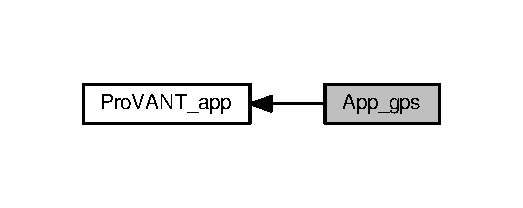
\includegraphics[width=251pt]{group__app__gps}
\end{center}
\end{figure}
\subsection*{Macros}
\begin{DoxyCompactItemize}
\item 
\#define \hyperlink{group__app__gps_ga0ac6c9f2991b096e49c354e5cce6fae0}{M\+O\+D\+U\+L\+E\+\_\+\+P\+E\+R\+I\+OD}~100
\end{DoxyCompactItemize}
\subsection*{Functions}
\begin{DoxyCompactItemize}
\item 
void \hyperlink{group__app__gps_ga9ee93102a0a5aec6877376bbcaf1dcb0}{module\+\_\+gps\+\_\+init} ()
\begin{DoxyCompactList}\small\item\em Inicializacao do módulo de G\+PS. \end{DoxyCompactList}\item 
void \hyperlink{group__app__gps_gace423457cfae0d22bd57db9e2fb4c033}{module\+\_\+gps\+\_\+run} ()
\begin{DoxyCompactList}\small\item\em Função principal do módulo de G\+PS. \end{DoxyCompactList}\end{DoxyCompactItemize}
\subsection*{Variables}
\begin{DoxyCompactItemize}
\item 
port\+Tick\+Type \hyperlink{group__app__gps_gaa8db3871cb5f64abbd94ddd5a1db73a6}{last\+Wake\+Time}
\item 
pv\+\_\+msg\+\_\+gps \hyperlink{group__app__gps_ga744821cc9c45de009ae70e6dc8d5e220}{o\+Gps\+Data}
\item 
pv\+\_\+msg\+\_\+control\+Output \hyperlink{group__app__gps_ga0a14ca4568444d2d76c256fa91585cdf}{o\+Control\+Output\+Data}
\end{DoxyCompactItemize}


\subsection{Detailed Description}
Módulo responsavel por tratar os dados do G\+PS. 

Definição do módulo de tratamento dos dados de G\+PS. 

\subsection{Macro Definition Documentation}
\index{App\+\_\+gps@{App\+\_\+gps}!M\+O\+D\+U\+L\+E\+\_\+\+P\+E\+R\+I\+OD@{M\+O\+D\+U\+L\+E\+\_\+\+P\+E\+R\+I\+OD}}
\index{M\+O\+D\+U\+L\+E\+\_\+\+P\+E\+R\+I\+OD@{M\+O\+D\+U\+L\+E\+\_\+\+P\+E\+R\+I\+OD}!App\+\_\+gps@{App\+\_\+gps}}
\subsubsection[{\texorpdfstring{M\+O\+D\+U\+L\+E\+\_\+\+P\+E\+R\+I\+OD}{MODULE_PERIOD}}]{\setlength{\rightskip}{0pt plus 5cm}\#define M\+O\+D\+U\+L\+E\+\_\+\+P\+E\+R\+I\+OD~100}\hypertarget{group__app__gps_ga0ac6c9f2991b096e49c354e5cce6fae0}{}\label{group__app__gps_ga0ac6c9f2991b096e49c354e5cce6fae0}


Definition at line 26 of file pv\+\_\+module\+\_\+gps.\+c.



\subsection{Function Documentation}
\index{App\+\_\+gps@{App\+\_\+gps}!module\+\_\+gps\+\_\+init@{module\+\_\+gps\+\_\+init}}
\index{module\+\_\+gps\+\_\+init@{module\+\_\+gps\+\_\+init}!App\+\_\+gps@{App\+\_\+gps}}
\subsubsection[{\texorpdfstring{module\+\_\+gps\+\_\+init()}{module_gps_init()}}]{\setlength{\rightskip}{0pt plus 5cm}void module\+\_\+gps\+\_\+init (
\begin{DoxyParamCaption}
{}
\end{DoxyParamCaption}
)}\hypertarget{group__app__gps_ga9ee93102a0a5aec6877376bbcaf1dcb0}{}\label{group__app__gps_ga9ee93102a0a5aec6877376bbcaf1dcb0}


Inicializacao do módulo de G\+PS. 

Instancia as Queues de comunicação inter-\/thread. 
\begin{DoxyParams}{Parameters}
{\em None} & \\
\hline
\end{DoxyParams}

\begin{DoxyRetVals}{Return values}
{\em None} & \\
\hline
\end{DoxyRetVals}


Definition at line 43 of file pv\+\_\+module\+\_\+gps.\+c.

\index{App\+\_\+gps@{App\+\_\+gps}!module\+\_\+gps\+\_\+run@{module\+\_\+gps\+\_\+run}}
\index{module\+\_\+gps\+\_\+run@{module\+\_\+gps\+\_\+run}!App\+\_\+gps@{App\+\_\+gps}}
\subsubsection[{\texorpdfstring{module\+\_\+gps\+\_\+run()}{module_gps_run()}}]{\setlength{\rightskip}{0pt plus 5cm}void module\+\_\+gps\+\_\+run (
\begin{DoxyParamCaption}
{}
\end{DoxyParamCaption}
)}\hypertarget{group__app__gps_gace423457cfae0d22bd57db9e2fb4c033}{}\label{group__app__gps_gace423457cfae0d22bd57db9e2fb4c033}


Função principal do módulo de G\+PS. 


\begin{DoxyParams}{Parameters}
{\em None} & \\
\hline
\end{DoxyParams}

\begin{DoxyRetVals}{Return values}
{\em None} & \\
\hline
\end{DoxyRetVals}


Definition at line 55 of file pv\+\_\+module\+\_\+gps.\+c.



\subsection{Variable Documentation}
\index{App\+\_\+gps@{App\+\_\+gps}!last\+Wake\+Time@{last\+Wake\+Time}}
\index{last\+Wake\+Time@{last\+Wake\+Time}!App\+\_\+gps@{App\+\_\+gps}}
\subsubsection[{\texorpdfstring{last\+Wake\+Time}{lastWakeTime}}]{\setlength{\rightskip}{0pt plus 5cm}port\+Tick\+Type last\+Wake\+Time}\hypertarget{group__app__gps_gaa8db3871cb5f64abbd94ddd5a1db73a6}{}\label{group__app__gps_gaa8db3871cb5f64abbd94ddd5a1db73a6}


Definition at line 30 of file pv\+\_\+module\+\_\+gps.\+c.

\index{App\+\_\+gps@{App\+\_\+gps}!o\+Control\+Output\+Data@{o\+Control\+Output\+Data}}
\index{o\+Control\+Output\+Data@{o\+Control\+Output\+Data}!App\+\_\+gps@{App\+\_\+gps}}
\subsubsection[{\texorpdfstring{o\+Control\+Output\+Data}{oControlOutputData}}]{\setlength{\rightskip}{0pt plus 5cm}pv\+\_\+msg\+\_\+control\+Output o\+Control\+Output\+Data}\hypertarget{group__app__gps_ga0a14ca4568444d2d76c256fa91585cdf}{}\label{group__app__gps_ga0a14ca4568444d2d76c256fa91585cdf}


Definition at line 32 of file pv\+\_\+module\+\_\+gps.\+c.

\index{App\+\_\+gps@{App\+\_\+gps}!o\+Gps\+Data@{o\+Gps\+Data}}
\index{o\+Gps\+Data@{o\+Gps\+Data}!App\+\_\+gps@{App\+\_\+gps}}
\subsubsection[{\texorpdfstring{o\+Gps\+Data}{oGpsData}}]{\setlength{\rightskip}{0pt plus 5cm}pv\+\_\+msg\+\_\+gps o\+Gps\+Data}\hypertarget{group__app__gps_ga744821cc9c45de009ae70e6dc8d5e220}{}\label{group__app__gps_ga744821cc9c45de009ae70e6dc8d5e220}


Definition at line 31 of file pv\+\_\+module\+\_\+gps.\+c.


\hypertarget{group__app__in}{}\section{App\+\_\+in}
\label{group__app__in}\index{App\+\_\+in@{App\+\_\+in}}


Componentes para o sensoriamento do V\+A\+NT.  


Collaboration diagram for App\+\_\+in\+:\nopagebreak
\begin{figure}[H]
\begin{center}
\leavevmode
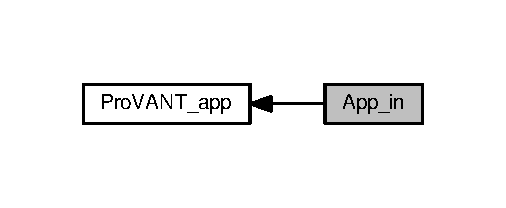
\includegraphics[width=243pt]{group__app__in}
\end{center}
\end{figure}
\subsection*{Macros}
\begin{DoxyCompactItemize}
\item 
\#define \hyperlink{group__app__in_ga0ac6c9f2991b096e49c354e5cce6fae0}{M\+O\+D\+U\+L\+E\+\_\+\+P\+E\+R\+I\+OD}~6
\end{DoxyCompactItemize}
\subsection*{Functions}
\begin{DoxyCompactItemize}
\item 
void \hyperlink{group__app__in_gaffe0980a750cbec13ebf241c933460dd}{module\+\_\+in\+\_\+init} ()
\begin{DoxyCompactList}\small\item\em Inicializacao componentes de IO. \end{DoxyCompactList}\item 
void \hyperlink{group__app__in_ga2b56089e4c5adb9ac8b7a41fc1a0b0b2}{module\+\_\+in\+\_\+run} ()
\begin{DoxyCompactList}\small\item\em Função principal do módulo de IO. \end{DoxyCompactList}\end{DoxyCompactItemize}
\subsection*{Variables}
\begin{DoxyCompactItemize}
\item 
port\+Tick\+Type \hyperlink{group__app__in_ga3ff9efc032b26284423c9100a5474b7b}{pv\+\_\+module\+\_\+in\+\_\+last\+Wake\+Time}
\item 
char \hyperlink{group__app__in_ga3000f858ecb5a5417c1566b691efd56d}{str} \mbox{[}256\mbox{]}
\item 
G\+P\+I\+O\+Pin \hyperlink{group__app__in_ga8d3f5e0ec53e4667efbebf11383765e4}{pv\+\_\+module\+\_\+in\+\_\+\+L\+E\+D4}
\item 
float \hyperlink{group__app__in_ga926ba5b807f8b3d71b9fb486eb32a508}{attitude\+\_\+quaternion} \mbox{[}4\mbox{]} =\{1,0,0,0\}
\item 
pv\+\_\+msg\+\_\+input \hyperlink{group__app__in_gaffc6f7805bab2d46af160c6f7715ba99}{o\+Input\+Data}
\end{DoxyCompactItemize}


\subsection{Detailed Description}
Componentes para o sensoriamento do V\+A\+NT. 

Reunião de todos os componentes relacionados às operações de input do V\+A\+NT. Leituras de todos os sensores. O processamento destes dados brutos é feito neste módulo. 

\subsection{Macro Definition Documentation}
\index{App\+\_\+in@{App\+\_\+in}!M\+O\+D\+U\+L\+E\+\_\+\+P\+E\+R\+I\+OD@{M\+O\+D\+U\+L\+E\+\_\+\+P\+E\+R\+I\+OD}}
\index{M\+O\+D\+U\+L\+E\+\_\+\+P\+E\+R\+I\+OD@{M\+O\+D\+U\+L\+E\+\_\+\+P\+E\+R\+I\+OD}!App\+\_\+in@{App\+\_\+in}}
\subsubsection[{\texorpdfstring{M\+O\+D\+U\+L\+E\+\_\+\+P\+E\+R\+I\+OD}{MODULE_PERIOD}}]{\setlength{\rightskip}{0pt plus 5cm}\#define M\+O\+D\+U\+L\+E\+\_\+\+P\+E\+R\+I\+OD~6}\hypertarget{group__app__in_ga0ac6c9f2991b096e49c354e5cce6fae0}{}\label{group__app__in_ga0ac6c9f2991b096e49c354e5cce6fae0}


Definition at line 28 of file pv\+\_\+module\+\_\+in.\+c.



\subsection{Function Documentation}
\index{App\+\_\+in@{App\+\_\+in}!module\+\_\+in\+\_\+init@{module\+\_\+in\+\_\+init}}
\index{module\+\_\+in\+\_\+init@{module\+\_\+in\+\_\+init}!App\+\_\+in@{App\+\_\+in}}
\subsubsection[{\texorpdfstring{module\+\_\+in\+\_\+init()}{module_in_init()}}]{\setlength{\rightskip}{0pt plus 5cm}void module\+\_\+in\+\_\+init (
\begin{DoxyParamCaption}
{}
\end{DoxyParamCaption}
)}\hypertarget{group__app__in_gaffe0980a750cbec13ebf241c933460dd}{}\label{group__app__in_gaffe0980a750cbec13ebf241c933460dd}


Inicializacao componentes de IO. 

Initializes the hardware to communicate with the sensors (I\+MU, S\+O\+N\+AR, R\+E\+C\+E\+I\+V\+ER, S\+E\+R\+V\+OS) Test routines still need to be performed. 
\begin{DoxyParams}{Parameters}
{\em None} & \\
\hline
\end{DoxyParams}

\begin{DoxyRetVals}{Return values}
{\em None} & \\
\hline
\end{DoxyRetVals}


Definition at line 55 of file pv\+\_\+module\+\_\+in.\+c.

\index{App\+\_\+in@{App\+\_\+in}!module\+\_\+in\+\_\+run@{module\+\_\+in\+\_\+run}}
\index{module\+\_\+in\+\_\+run@{module\+\_\+in\+\_\+run}!App\+\_\+in@{App\+\_\+in}}
\subsubsection[{\texorpdfstring{module\+\_\+in\+\_\+run()}{module_in_run()}}]{\setlength{\rightskip}{0pt plus 5cm}void module\+\_\+in\+\_\+run (
\begin{DoxyParamCaption}
{}
\end{DoxyParamCaption}
)}\hypertarget{group__app__in_ga2b56089e4c5adb9ac8b7a41fc1a0b0b2}{}\label{group__app__in_ga2b56089e4c5adb9ac8b7a41fc1a0b0b2}


Função principal do módulo de IO. 


\begin{DoxyParams}{Parameters}
{\em None} & \\
\hline
\end{DoxyParams}

\begin{DoxyRetVals}{Return values}
{\em None} & Loop que amostra sensores como necessário. \\
\hline
\end{DoxyRetVals}


Definition at line 90 of file pv\+\_\+module\+\_\+in.\+c.



\subsection{Variable Documentation}
\index{App\+\_\+in@{App\+\_\+in}!attitude\+\_\+quaternion@{attitude\+\_\+quaternion}}
\index{attitude\+\_\+quaternion@{attitude\+\_\+quaternion}!App\+\_\+in@{App\+\_\+in}}
\subsubsection[{\texorpdfstring{attitude\+\_\+quaternion}{attitude_quaternion}}]{\setlength{\rightskip}{0pt plus 5cm}float attitude\+\_\+quaternion\mbox{[}4\mbox{]} =\{1,0,0,0\}}\hypertarget{group__app__in_ga926ba5b807f8b3d71b9fb486eb32a508}{}\label{group__app__in_ga926ba5b807f8b3d71b9fb486eb32a508}


Definition at line 37 of file pv\+\_\+module\+\_\+in.\+c.

\index{App\+\_\+in@{App\+\_\+in}!o\+Input\+Data@{o\+Input\+Data}}
\index{o\+Input\+Data@{o\+Input\+Data}!App\+\_\+in@{App\+\_\+in}}
\subsubsection[{\texorpdfstring{o\+Input\+Data}{oInputData}}]{\setlength{\rightskip}{0pt plus 5cm}pv\+\_\+msg\+\_\+input o\+Input\+Data}\hypertarget{group__app__in_gaffc6f7805bab2d46af160c6f7715ba99}{}\label{group__app__in_gaffc6f7805bab2d46af160c6f7715ba99}


Definition at line 41 of file pv\+\_\+module\+\_\+in.\+c.

\index{App\+\_\+in@{App\+\_\+in}!pv\+\_\+module\+\_\+in\+\_\+last\+Wake\+Time@{pv\+\_\+module\+\_\+in\+\_\+last\+Wake\+Time}}
\index{pv\+\_\+module\+\_\+in\+\_\+last\+Wake\+Time@{pv\+\_\+module\+\_\+in\+\_\+last\+Wake\+Time}!App\+\_\+in@{App\+\_\+in}}
\subsubsection[{\texorpdfstring{pv\+\_\+module\+\_\+in\+\_\+last\+Wake\+Time}{pv_module_in_lastWakeTime}}]{\setlength{\rightskip}{0pt plus 5cm}port\+Tick\+Type pv\+\_\+module\+\_\+in\+\_\+last\+Wake\+Time}\hypertarget{group__app__in_ga3ff9efc032b26284423c9100a5474b7b}{}\label{group__app__in_ga3ff9efc032b26284423c9100a5474b7b}


Definition at line 33 of file pv\+\_\+module\+\_\+in.\+c.

\index{App\+\_\+in@{App\+\_\+in}!pv\+\_\+module\+\_\+in\+\_\+\+L\+E\+D4@{pv\+\_\+module\+\_\+in\+\_\+\+L\+E\+D4}}
\index{pv\+\_\+module\+\_\+in\+\_\+\+L\+E\+D4@{pv\+\_\+module\+\_\+in\+\_\+\+L\+E\+D4}!App\+\_\+in@{App\+\_\+in}}
\subsubsection[{\texorpdfstring{pv\+\_\+module\+\_\+in\+\_\+\+L\+E\+D4}{pv_module_in_LED4}}]{\setlength{\rightskip}{0pt plus 5cm}G\+P\+I\+O\+Pin pv\+\_\+module\+\_\+in\+\_\+\+L\+E\+D4}\hypertarget{group__app__in_ga8d3f5e0ec53e4667efbebf11383765e4}{}\label{group__app__in_ga8d3f5e0ec53e4667efbebf11383765e4}


Definition at line 35 of file pv\+\_\+module\+\_\+in.\+c.

\index{App\+\_\+in@{App\+\_\+in}!str@{str}}
\index{str@{str}!App\+\_\+in@{App\+\_\+in}}
\subsubsection[{\texorpdfstring{str}{str}}]{\setlength{\rightskip}{0pt plus 5cm}char str\mbox{[}256\mbox{]}}\hypertarget{group__app__in_ga3000f858ecb5a5417c1566b691efd56d}{}\label{group__app__in_ga3000f858ecb5a5417c1566b691efd56d}


Definition at line 34 of file pv\+\_\+module\+\_\+in.\+c.


\hypertarget{group__app__sm}{}\section{App\+\_\+sm}
\label{group__app__sm}\index{App\+\_\+sm@{App\+\_\+sm}}


Módulo responsavel pela maquina de estados do V\+A\+NT.  


Collaboration diagram for App\+\_\+sm\+:\nopagebreak
\begin{figure}[H]
\begin{center}
\leavevmode
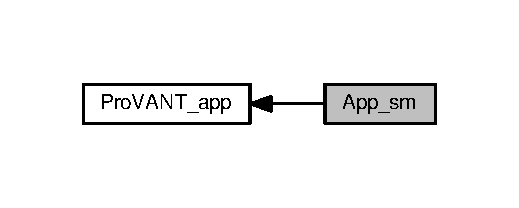
\includegraphics[width=249pt]{group__app__sm}
\end{center}
\end{figure}
\subsection*{Macros}
\begin{DoxyCompactItemize}
\item 
\#define \hyperlink{group__app__sm_ga0ac6c9f2991b096e49c354e5cce6fae0}{M\+O\+D\+U\+L\+E\+\_\+\+P\+E\+R\+I\+OD}~20
\end{DoxyCompactItemize}
\subsection*{Functions}
\begin{DoxyCompactItemize}
\item 
void \hyperlink{group__app__sm_gaf1b95b5ff451c9c5d9a4cdd34531201b}{module\+\_\+sm\+\_\+init} ()
\begin{DoxyCompactList}\small\item\em Inicializacao do módulo de sm. \end{DoxyCompactList}\item 
void \hyperlink{group__app__sm_ga81e54a060d460608697719ba6afab1e4}{module\+\_\+sm\+\_\+run} ()
\begin{DoxyCompactList}\small\item\em Função principal do módulo da sm. \end{DoxyCompactList}\end{DoxyCompactItemize}
\subsection*{Variables}
\begin{DoxyCompactItemize}
\item 
port\+Tick\+Type \hyperlink{group__app__sm_gaa8db3871cb5f64abbd94ddd5a1db73a6}{last\+Wake\+Time}
\end{DoxyCompactItemize}


\subsection{Detailed Description}
Módulo responsavel pela maquina de estados do V\+A\+NT. 

Definição do módulo da maquina de estados. 

\subsection{Macro Definition Documentation}
\index{App\+\_\+sm@{App\+\_\+sm}!M\+O\+D\+U\+L\+E\+\_\+\+P\+E\+R\+I\+OD@{M\+O\+D\+U\+L\+E\+\_\+\+P\+E\+R\+I\+OD}}
\index{M\+O\+D\+U\+L\+E\+\_\+\+P\+E\+R\+I\+OD@{M\+O\+D\+U\+L\+E\+\_\+\+P\+E\+R\+I\+OD}!App\+\_\+sm@{App\+\_\+sm}}
\subsubsection[{\texorpdfstring{M\+O\+D\+U\+L\+E\+\_\+\+P\+E\+R\+I\+OD}{MODULE_PERIOD}}]{\setlength{\rightskip}{0pt plus 5cm}\#define M\+O\+D\+U\+L\+E\+\_\+\+P\+E\+R\+I\+OD~20}\hypertarget{group__app__sm_ga0ac6c9f2991b096e49c354e5cce6fae0}{}\label{group__app__sm_ga0ac6c9f2991b096e49c354e5cce6fae0}


Definition at line 26 of file pv\+\_\+module\+\_\+sm.\+c.



\subsection{Function Documentation}
\index{App\+\_\+sm@{App\+\_\+sm}!module\+\_\+sm\+\_\+init@{module\+\_\+sm\+\_\+init}}
\index{module\+\_\+sm\+\_\+init@{module\+\_\+sm\+\_\+init}!App\+\_\+sm@{App\+\_\+sm}}
\subsubsection[{\texorpdfstring{module\+\_\+sm\+\_\+init()}{module_sm_init()}}]{\setlength{\rightskip}{0pt plus 5cm}void module\+\_\+sm\+\_\+init (
\begin{DoxyParamCaption}
{}
\end{DoxyParamCaption}
)}\hypertarget{group__app__sm_gaf1b95b5ff451c9c5d9a4cdd34531201b}{}\label{group__app__sm_gaf1b95b5ff451c9c5d9a4cdd34531201b}


Inicializacao do módulo de sm. 

Instancia as Queues de comunicação inter-\/thread. 
\begin{DoxyParams}{Parameters}
{\em None} & \\
\hline
\end{DoxyParams}

\begin{DoxyRetVals}{Return values}
{\em None} & \\
\hline
\end{DoxyRetVals}


Definition at line 41 of file pv\+\_\+module\+\_\+sm.\+c.

\index{App\+\_\+sm@{App\+\_\+sm}!module\+\_\+sm\+\_\+run@{module\+\_\+sm\+\_\+run}}
\index{module\+\_\+sm\+\_\+run@{module\+\_\+sm\+\_\+run}!App\+\_\+sm@{App\+\_\+sm}}
\subsubsection[{\texorpdfstring{module\+\_\+sm\+\_\+run()}{module_sm_run()}}]{\setlength{\rightskip}{0pt plus 5cm}void module\+\_\+sm\+\_\+run (
\begin{DoxyParamCaption}
{}
\end{DoxyParamCaption}
)}\hypertarget{group__app__sm_ga81e54a060d460608697719ba6afab1e4}{}\label{group__app__sm_ga81e54a060d460608697719ba6afab1e4}


Função principal do módulo da sm. 


\begin{DoxyParams}{Parameters}
{\em None} & \\
\hline
\end{DoxyParams}

\begin{DoxyRetVals}{Return values}
{\em None} & \\
\hline
\end{DoxyRetVals}


Definition at line 50 of file pv\+\_\+module\+\_\+sm.\+c.



\subsection{Variable Documentation}
\index{App\+\_\+sm@{App\+\_\+sm}!last\+Wake\+Time@{last\+Wake\+Time}}
\index{last\+Wake\+Time@{last\+Wake\+Time}!App\+\_\+sm@{App\+\_\+sm}}
\subsubsection[{\texorpdfstring{last\+Wake\+Time}{lastWakeTime}}]{\setlength{\rightskip}{0pt plus 5cm}port\+Tick\+Type last\+Wake\+Time}\hypertarget{group__app__sm_gaa8db3871cb5f64abbd94ddd5a1db73a6}{}\label{group__app__sm_gaa8db3871cb5f64abbd94ddd5a1db73a6}


Definition at line 30 of file pv\+\_\+module\+\_\+sm.\+c.


\chapter{Data Structure Documentation}
\hypertarget{structpv__interface__co}{}\section{pv\+\_\+interface\+\_\+co Struct Reference}
\label{structpv__interface__co}\index{pv\+\_\+interface\+\_\+co@{pv\+\_\+interface\+\_\+co}}


{\ttfamily \#include $<$pv\+\_\+module\+\_\+co.\+h$>$}



Collaboration diagram for pv\+\_\+interface\+\_\+co\+:\nopagebreak
\begin{figure}[H]
\begin{center}
\leavevmode
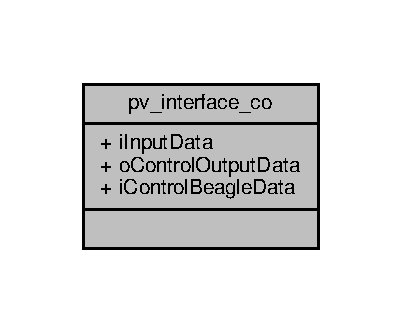
\includegraphics[width=193pt]{structpv__interface__co__coll__graph}
\end{center}
\end{figure}
\subsection*{Data Fields}
\begin{DoxyCompactItemize}
\item 
x\+Queue\+Handle \hyperlink{structpv__interface__co_ad057767ef15274f0933ad1821fea7239}{i\+Input\+Data}
\item 
x\+Queue\+Handle \hyperlink{structpv__interface__co_adeb92ab25c31742c709ae51f96cbf10a}{o\+Control\+Output\+Data}
\item 
x\+Queue\+Handle \hyperlink{structpv__interface__co_a0d6eb6afadef31d21002472d9e7266f9}{i\+Control\+Beagle\+Data}
\end{DoxyCompactItemize}


\subsection{Detailed Description}


Definition at line 41 of file pv\+\_\+module\+\_\+co.\+h.



\subsection{Field Documentation}
\index{pv\+\_\+interface\+\_\+co@{pv\+\_\+interface\+\_\+co}!i\+Control\+Beagle\+Data@{i\+Control\+Beagle\+Data}}
\index{i\+Control\+Beagle\+Data@{i\+Control\+Beagle\+Data}!pv\+\_\+interface\+\_\+co@{pv\+\_\+interface\+\_\+co}}
\subsubsection[{\texorpdfstring{i\+Control\+Beagle\+Data}{iControlBeagleData}}]{\setlength{\rightskip}{0pt plus 5cm}x\+Queue\+Handle i\+Control\+Beagle\+Data}\hypertarget{structpv__interface__co_a0d6eb6afadef31d21002472d9e7266f9}{}\label{structpv__interface__co_a0d6eb6afadef31d21002472d9e7266f9}


Definition at line 45 of file pv\+\_\+module\+\_\+co.\+h.

\index{pv\+\_\+interface\+\_\+co@{pv\+\_\+interface\+\_\+co}!i\+Input\+Data@{i\+Input\+Data}}
\index{i\+Input\+Data@{i\+Input\+Data}!pv\+\_\+interface\+\_\+co@{pv\+\_\+interface\+\_\+co}}
\subsubsection[{\texorpdfstring{i\+Input\+Data}{iInputData}}]{\setlength{\rightskip}{0pt plus 5cm}x\+Queue\+Handle i\+Input\+Data}\hypertarget{structpv__interface__co_ad057767ef15274f0933ad1821fea7239}{}\label{structpv__interface__co_ad057767ef15274f0933ad1821fea7239}


Definition at line 43 of file pv\+\_\+module\+\_\+co.\+h.

\index{pv\+\_\+interface\+\_\+co@{pv\+\_\+interface\+\_\+co}!o\+Control\+Output\+Data@{o\+Control\+Output\+Data}}
\index{o\+Control\+Output\+Data@{o\+Control\+Output\+Data}!pv\+\_\+interface\+\_\+co@{pv\+\_\+interface\+\_\+co}}
\subsubsection[{\texorpdfstring{o\+Control\+Output\+Data}{oControlOutputData}}]{\setlength{\rightskip}{0pt plus 5cm}x\+Queue\+Handle o\+Control\+Output\+Data}\hypertarget{structpv__interface__co_adeb92ab25c31742c709ae51f96cbf10a}{}\label{structpv__interface__co_adeb92ab25c31742c709ae51f96cbf10a}


Definition at line 44 of file pv\+\_\+module\+\_\+co.\+h.



The documentation for this struct was generated from the following file\+:\begin{DoxyCompactItemize}
\item 
/home/provant/\+Documents/provant-\/software/io-\/board/stm32f4/app/remote-\/controlled-\/flight/\hyperlink{pv__module__co_8h}{pv\+\_\+module\+\_\+co.\+h}\end{DoxyCompactItemize}

\hypertarget{structpv__interface__do}{}\section{pv\+\_\+interface\+\_\+do Struct Reference}
\label{structpv__interface__do}\index{pv\+\_\+interface\+\_\+do@{pv\+\_\+interface\+\_\+do}}


{\ttfamily \#include $<$pv\+\_\+module\+\_\+do.\+h$>$}



Collaboration diagram for pv\+\_\+interface\+\_\+do\+:\nopagebreak
\begin{figure}[H]
\begin{center}
\leavevmode
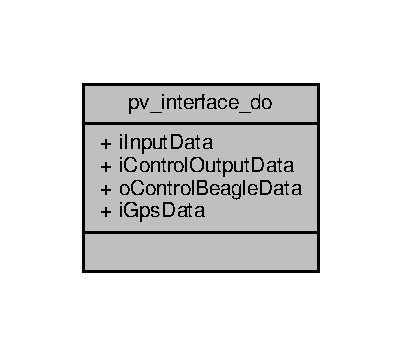
\includegraphics[width=193pt]{structpv__interface__do__coll__graph}
\end{center}
\end{figure}
\subsection*{Data Fields}
\begin{DoxyCompactItemize}
\item 
x\+Queue\+Handle \hyperlink{structpv__interface__do_ad057767ef15274f0933ad1821fea7239}{i\+Input\+Data}
\item 
x\+Queue\+Handle \hyperlink{structpv__interface__do_a47359dc53fe6c9e48eae67c40f5bde8a}{i\+Control\+Output\+Data}
\item 
x\+Queue\+Handle \hyperlink{structpv__interface__do_a4ed79d3529d7b97899602893078332b0}{o\+Control\+Beagle\+Data}
\item 
x\+Queue\+Handle \hyperlink{structpv__interface__do_a98e72320f39ff4a7ec39da06b878ff1b}{i\+Gps\+Data}
\end{DoxyCompactItemize}


\subsection{Detailed Description}


Definition at line 36 of file pv\+\_\+module\+\_\+do.\+h.



\subsection{Field Documentation}
\index{pv\+\_\+interface\+\_\+do@{pv\+\_\+interface\+\_\+do}!i\+Control\+Output\+Data@{i\+Control\+Output\+Data}}
\index{i\+Control\+Output\+Data@{i\+Control\+Output\+Data}!pv\+\_\+interface\+\_\+do@{pv\+\_\+interface\+\_\+do}}
\subsubsection[{\texorpdfstring{i\+Control\+Output\+Data}{iControlOutputData}}]{\setlength{\rightskip}{0pt plus 5cm}x\+Queue\+Handle i\+Control\+Output\+Data}\hypertarget{structpv__interface__do_a47359dc53fe6c9e48eae67c40f5bde8a}{}\label{structpv__interface__do_a47359dc53fe6c9e48eae67c40f5bde8a}


Definition at line 39 of file pv\+\_\+module\+\_\+do.\+h.

\index{pv\+\_\+interface\+\_\+do@{pv\+\_\+interface\+\_\+do}!i\+Gps\+Data@{i\+Gps\+Data}}
\index{i\+Gps\+Data@{i\+Gps\+Data}!pv\+\_\+interface\+\_\+do@{pv\+\_\+interface\+\_\+do}}
\subsubsection[{\texorpdfstring{i\+Gps\+Data}{iGpsData}}]{\setlength{\rightskip}{0pt plus 5cm}x\+Queue\+Handle i\+Gps\+Data}\hypertarget{structpv__interface__do_a98e72320f39ff4a7ec39da06b878ff1b}{}\label{structpv__interface__do_a98e72320f39ff4a7ec39da06b878ff1b}


Definition at line 41 of file pv\+\_\+module\+\_\+do.\+h.

\index{pv\+\_\+interface\+\_\+do@{pv\+\_\+interface\+\_\+do}!i\+Input\+Data@{i\+Input\+Data}}
\index{i\+Input\+Data@{i\+Input\+Data}!pv\+\_\+interface\+\_\+do@{pv\+\_\+interface\+\_\+do}}
\subsubsection[{\texorpdfstring{i\+Input\+Data}{iInputData}}]{\setlength{\rightskip}{0pt plus 5cm}x\+Queue\+Handle i\+Input\+Data}\hypertarget{structpv__interface__do_ad057767ef15274f0933ad1821fea7239}{}\label{structpv__interface__do_ad057767ef15274f0933ad1821fea7239}


Definition at line 38 of file pv\+\_\+module\+\_\+do.\+h.

\index{pv\+\_\+interface\+\_\+do@{pv\+\_\+interface\+\_\+do}!o\+Control\+Beagle\+Data@{o\+Control\+Beagle\+Data}}
\index{o\+Control\+Beagle\+Data@{o\+Control\+Beagle\+Data}!pv\+\_\+interface\+\_\+do@{pv\+\_\+interface\+\_\+do}}
\subsubsection[{\texorpdfstring{o\+Control\+Beagle\+Data}{oControlBeagleData}}]{\setlength{\rightskip}{0pt plus 5cm}x\+Queue\+Handle o\+Control\+Beagle\+Data}\hypertarget{structpv__interface__do_a4ed79d3529d7b97899602893078332b0}{}\label{structpv__interface__do_a4ed79d3529d7b97899602893078332b0}


Definition at line 40 of file pv\+\_\+module\+\_\+do.\+h.



The documentation for this struct was generated from the following file\+:\begin{DoxyCompactItemize}
\item 
/home/provant/\+Documents/provant-\/software/io-\/board/stm32f4/app/remote-\/controlled-\/flight/\hyperlink{pv__module__do_8h}{pv\+\_\+module\+\_\+do.\+h}\end{DoxyCompactItemize}

\hypertarget{structpv__interface__gps}{}\section{pv\+\_\+interface\+\_\+gps Struct Reference}
\label{structpv__interface__gps}\index{pv\+\_\+interface\+\_\+gps@{pv\+\_\+interface\+\_\+gps}}


{\ttfamily \#include $<$pv\+\_\+module\+\_\+gps.\+h$>$}



Collaboration diagram for pv\+\_\+interface\+\_\+gps\+:\nopagebreak
\begin{figure}[H]
\begin{center}
\leavevmode
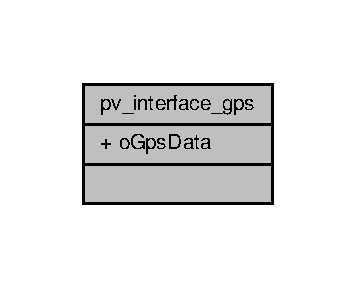
\includegraphics[width=171pt]{structpv__interface__gps__coll__graph}
\end{center}
\end{figure}
\subsection*{Data Fields}
\begin{DoxyCompactItemize}
\item 
x\+Queue\+Handle \hyperlink{structpv__interface__gps_a4e4f88e8b52f49bd7ceae60e2660f406}{o\+Gps\+Data}
\end{DoxyCompactItemize}


\subsection{Detailed Description}


Definition at line 36 of file pv\+\_\+module\+\_\+gps.\+h.



\subsection{Field Documentation}
\index{pv\+\_\+interface\+\_\+gps@{pv\+\_\+interface\+\_\+gps}!o\+Gps\+Data@{o\+Gps\+Data}}
\index{o\+Gps\+Data@{o\+Gps\+Data}!pv\+\_\+interface\+\_\+gps@{pv\+\_\+interface\+\_\+gps}}
\subsubsection[{\texorpdfstring{o\+Gps\+Data}{oGpsData}}]{\setlength{\rightskip}{0pt plus 5cm}x\+Queue\+Handle o\+Gps\+Data}\hypertarget{structpv__interface__gps_a4e4f88e8b52f49bd7ceae60e2660f406}{}\label{structpv__interface__gps_a4e4f88e8b52f49bd7ceae60e2660f406}


Definition at line 38 of file pv\+\_\+module\+\_\+gps.\+h.



The documentation for this struct was generated from the following file\+:\begin{DoxyCompactItemize}
\item 
/home/provant/\+Documents/provant-\/software/io-\/board/stm32f4/app/remote-\/controlled-\/flight/\hyperlink{pv__module__gps_8h}{pv\+\_\+module\+\_\+gps.\+h}\end{DoxyCompactItemize}

\hypertarget{structpv__interface__in}{}\section{pv\+\_\+interface\+\_\+in Struct Reference}
\label{structpv__interface__in}\index{pv\+\_\+interface\+\_\+in@{pv\+\_\+interface\+\_\+in}}


{\ttfamily \#include $<$pv\+\_\+module\+\_\+in.\+h$>$}



Collaboration diagram for pv\+\_\+interface\+\_\+in\+:\nopagebreak
\begin{figure}[H]
\begin{center}
\leavevmode
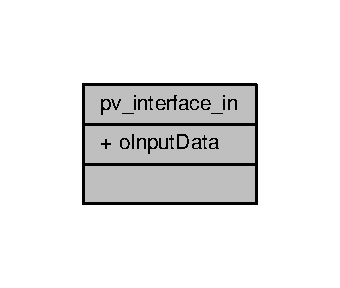
\includegraphics[width=163pt]{structpv__interface__in__coll__graph}
\end{center}
\end{figure}
\subsection*{Data Fields}
\begin{DoxyCompactItemize}
\item 
x\+Queue\+Handle \hyperlink{structpv__interface__in_a1b28b7bd6ca96936bf91240eea51d3b9}{o\+Input\+Data}
\end{DoxyCompactItemize}


\subsection{Detailed Description}


Definition at line 82 of file pv\+\_\+module\+\_\+in.\+h.



\subsection{Field Documentation}
\index{pv\+\_\+interface\+\_\+in@{pv\+\_\+interface\+\_\+in}!o\+Input\+Data@{o\+Input\+Data}}
\index{o\+Input\+Data@{o\+Input\+Data}!pv\+\_\+interface\+\_\+in@{pv\+\_\+interface\+\_\+in}}
\subsubsection[{\texorpdfstring{o\+Input\+Data}{oInputData}}]{\setlength{\rightskip}{0pt plus 5cm}x\+Queue\+Handle o\+Input\+Data}\hypertarget{structpv__interface__in_a1b28b7bd6ca96936bf91240eea51d3b9}{}\label{structpv__interface__in_a1b28b7bd6ca96936bf91240eea51d3b9}


Definition at line 84 of file pv\+\_\+module\+\_\+in.\+h.



The documentation for this struct was generated from the following file\+:\begin{DoxyCompactItemize}
\item 
/home/provant/\+Documents/provant-\/software/io-\/board/stm32f4/app/remote-\/controlled-\/flight/\hyperlink{pv__module__in_8h}{pv\+\_\+module\+\_\+in.\+h}\end{DoxyCompactItemize}

\chapter{File Documentation}
\hypertarget{CMakeLists_8txt}{}\section{/home/provant/\+Documents/provant-\/software/io-\/board/stm32f4/app/remote-\/controlled-\/flight/\+C\+Make\+Lists.txt File Reference}
\label{CMakeLists_8txt}\index{/home/provant/\+Documents/provant-\/software/io-\/board/stm32f4/app/remote-\/controlled-\/flight/\+C\+Make\+Lists.\+txt@{/home/provant/\+Documents/provant-\/software/io-\/board/stm32f4/app/remote-\/controlled-\/flight/\+C\+Make\+Lists.\+txt}}
\subsection*{Functions}
\begin{DoxyCompactItemize}
\item 
\hyperlink{CMakeLists_8txt_aef80c282ddc0836d69df376060234fce}{cmake\+\_\+minimum\+\_\+required} (V\+E\+R\+S\+I\+ON 2.\+8.\+3) cmake\+\_\+policy(S\+ET C\+M\+P0037 O\+LD) \hyperlink{CMakeLists_8txt_a6ff7757e73646eb491e3cd678902beed}{set}(P\+R\+O\+J\+E\+C\+T\+\_\+\+N\+A\+ME remote-\/controlled-\/flight) \hyperlink{CMakeLists_8txt_a6ff7757e73646eb491e3cd678902beed}{set}(A\+P\+P\+D\+IR\char`\"{}\$
\item 
\hyperlink{CMakeLists_8txt_a8ccd63c3a8ce266e619619ed30262689}{set} (O\+U\+T\+D\+IR\char`\"{}\$\{C\+M\+A\+K\+E\+\_\+\+C\+U\+R\+R\+E\+N\+T\+\_\+\+L\+I\+S\+T\+\_\+\+D\+IR\}/buildtest\char`\"{}) set(C\+O\+RE\char`\"{}\$
\item 
core \hyperlink{CMakeLists_8txt_adad964fe5734f8fa97709cda2d1d1203}{set} (B\+A\+SE\char`\"{}\$\{C\+M\+A\+K\+E\+\_\+\+C\+U\+R\+R\+E\+N\+T\+\_\+\+L\+I\+S\+T\+\_\+\+D\+IR\}/../../base\char`\"{}) set(C\+M\+S\+I\+S\+D\+IR\char`\"{}\$
\item 
cmsis \hyperlink{CMakeLists_8txt_aa1cb6cbed720134dafc50fe60197c62c}{set} (C\+M\+S\+I\+S\+S\+R\+C\+D\+IR\char`\"{}\$\{C\+M\+S\+I\+S\+D\+IR\}/src\char`\"{}) set(C\+M\+S\+I\+S\+I\+N\+C\+D\+IR\char`\"{}\$
\item 
inc \hyperlink{CMakeLists_8txt_a5eefef341371ecbbd5acbb9106123ddd}{set} (D\+S\+P\+D\+IR\char`\"{}\$\{C\+O\+RE\}/D\+S\+P\+\_\+\+Lib\char`\"{}) set(D\+S\+P\+S\+RC\char`\"{}\$
\item 
Source \hyperlink{CMakeLists_8txt_aad905f700e203964e09916a72c7db0d0}{set} (D\+S\+P\+L\+IB\char`\"{}\$\{D\+S\+P\+D\+IR\}/Lib/\char`\"{}) set(F\+R\+T\+D\+IR\char`\"{}\$
\item 
Free\+R\+T\+O\+S\+V7 Free\+R\+T\+OS \hyperlink{CMakeLists_8txt_acfd28e84a5e2c6910adf4fa1aee99b25}{set} (F\+R\+T\+S\+R\+C\+D\+IR\char`\"{}\$\{F\+R\+T\+D\+IR\}/Source\char`\"{}) set(F\+R\+T\+I\+N\+C\+D\+IR\char`\"{}\$
\item 
include \hyperlink{CMakeLists_8txt_a6ff7757e73646eb491e3cd678902beed}{set} (F\+R\+T\+M\+E\+M\+D\+IR\char`\"{}\$\{F\+R\+T\+S\+R\+C\+D\+IR\}/portable/Mem\+Mang/\char`\"{}) set(F\+R\+T\+P\+O\+R\+D\+IR\char`\"{}\$
\end{DoxyCompactItemize}


\subsection{Function Documentation}
\index{C\+Make\+Lists.\+txt@{C\+Make\+Lists.\+txt}!cmake\+\_\+minimum\+\_\+required@{cmake\+\_\+minimum\+\_\+required}}
\index{cmake\+\_\+minimum\+\_\+required@{cmake\+\_\+minimum\+\_\+required}!C\+Make\+Lists.\+txt@{C\+Make\+Lists.\+txt}}
\subsubsection[{\texorpdfstring{cmake\+\_\+minimum\+\_\+required(\+V\+E\+R\+S\+I\+O\+N 2.\+8.\+3) cmake\+\_\+policy(\+S\+E\+T C\+M\+P0037 O\+L\+D) set(\+P\+R\+O\+J\+E\+C\+T\+\_\+\+N\+A\+M\+E remote-\/controlled-\/flight) set(\+A\+P\+P\+D\+IR""\$}{cmake_minimum_required(VERSION 2.8.3) cmake_policy(SET CMP0037 OLD) set(PROJECT_NAME remote-controlled-flight) set(APPDIR"$}}]{\setlength{\rightskip}{0pt plus 5cm}cmake\+\_\+minimum\+\_\+required (
\begin{DoxyParamCaption}
\item[{V\+E\+R\+S\+I\+ON 2.\+8.}]{3}
\end{DoxyParamCaption}
)}\hypertarget{CMakeLists_8txt_aef80c282ddc0836d69df376060234fce}{}\label{CMakeLists_8txt_aef80c282ddc0836d69df376060234fce}


Definition at line 23 of file C\+Make\+Lists.\+txt.

\index{C\+Make\+Lists.\+txt@{C\+Make\+Lists.\+txt}!set@{set}}
\index{set@{set}!C\+Make\+Lists.\+txt@{C\+Make\+Lists.\+txt}}
\subsubsection[{\texorpdfstring{set(\+O\+U\+T\+D\+IR""\$\lcurly{}C\+M\+A\+K\+E\+\_\+\+C\+U\+R\+R\+E\+N\+T\+\_\+\+L\+I\+S\+T\+\_\+\+D\+IR\rcurly{}/buildtest"") set(\+C\+O\+RE""\$}{set(OUTDIR"$\{CMAKE_CURRENT_LIST_DIR\}/buildtest") set(CORE"$}}]{\setlength{\rightskip}{0pt plus 5cm}set (
\begin{DoxyParamCaption}
\item[{O\+U\+T\+D\+IR\char`\"{}\$\{C\+M\+A\+K\+E\+\_\+\+C\+U\+R\+R\+E\+N\+T\+\_\+\+L\+I\+S\+T\+\_\+\+D\+IR\}/buildtest\char`\"{}}]{}
\end{DoxyParamCaption}
)}\hypertarget{CMakeLists_8txt_a8ccd63c3a8ce266e619619ed30262689}{}\label{CMakeLists_8txt_a8ccd63c3a8ce266e619619ed30262689}


Definition at line 30 of file C\+Make\+Lists.\+txt.

\index{C\+Make\+Lists.\+txt@{C\+Make\+Lists.\+txt}!set@{set}}
\index{set@{set}!C\+Make\+Lists.\+txt@{C\+Make\+Lists.\+txt}}
\subsubsection[{\texorpdfstring{set(\+B\+A\+SE""\$\lcurly{}C\+M\+A\+K\+E\+\_\+\+C\+U\+R\+R\+E\+N\+T\+\_\+\+L\+I\+S\+T\+\_\+\+D\+IR\rcurly{}/../../base"") set(\+C\+M\+S\+I\+S\+D\+IR""\$}{set(BASE"$\{CMAKE_CURRENT_LIST_DIR\}/../../base") set(CMSISDIR"$}}]{\setlength{\rightskip}{0pt plus 5cm}core set (
\begin{DoxyParamCaption}
\item[{B\+A\+SE\char`\"{}\$\{C\+M\+A\+K\+E\+\_\+\+C\+U\+R\+R\+E\+N\+T\+\_\+\+L\+I\+S\+T\+\_\+\+D\+IR\}/../../base\char`\"{}}]{}
\end{DoxyParamCaption}
)}\hypertarget{CMakeLists_8txt_adad964fe5734f8fa97709cda2d1d1203}{}\label{CMakeLists_8txt_adad964fe5734f8fa97709cda2d1d1203}


Definition at line 32 of file C\+Make\+Lists.\+txt.

\index{C\+Make\+Lists.\+txt@{C\+Make\+Lists.\+txt}!set@{set}}
\index{set@{set}!C\+Make\+Lists.\+txt@{C\+Make\+Lists.\+txt}}
\subsubsection[{\texorpdfstring{set(\+C\+M\+S\+I\+S\+S\+R\+C\+D\+IR""\$\lcurly{}C\+M\+S\+I\+S\+D\+IR\rcurly{}/src"") set(\+C\+M\+S\+I\+S\+I\+N\+C\+D\+IR""\$}{set(CMSISSRCDIR"$\{CMSISDIR\}/src") set(CMSISINCDIR"$}}]{\setlength{\rightskip}{0pt plus 5cm}cmsis set (
\begin{DoxyParamCaption}
\item[{C\+M\+S\+I\+S\+S\+R\+C\+D\+IR\char`\"{}\$\{C\+M\+S\+I\+S\+D\+IR\}/src\char`\"{}}]{}
\end{DoxyParamCaption}
)}\hypertarget{CMakeLists_8txt_aa1cb6cbed720134dafc50fe60197c62c}{}\label{CMakeLists_8txt_aa1cb6cbed720134dafc50fe60197c62c}


Definition at line 36 of file C\+Make\+Lists.\+txt.

\index{C\+Make\+Lists.\+txt@{C\+Make\+Lists.\+txt}!set@{set}}
\index{set@{set}!C\+Make\+Lists.\+txt@{C\+Make\+Lists.\+txt}}
\subsubsection[{\texorpdfstring{set(\+D\+S\+P\+D\+IR""\$\lcurly{}C\+O\+RE\rcurly{}/\+D\+S\+P\+\_\+\+Lib"") set(\+D\+S\+P\+S\+RC""\$}{set(DSPDIR"$\{CORE\}/DSP_Lib") set(DSPSRC"$}}]{\setlength{\rightskip}{0pt plus 5cm}inc set (
\begin{DoxyParamCaption}
\item[{D\+S\+P\+D\+IR\char`\"{}\$\{C\+O\+RE\}/D\+S\+P\+\_\+\+Lib\char`\"{}}]{}
\end{DoxyParamCaption}
)}\hypertarget{CMakeLists_8txt_a5eefef341371ecbbd5acbb9106123ddd}{}\label{CMakeLists_8txt_a5eefef341371ecbbd5acbb9106123ddd}


Definition at line 40 of file C\+Make\+Lists.\+txt.

\index{C\+Make\+Lists.\+txt@{C\+Make\+Lists.\+txt}!set@{set}}
\index{set@{set}!C\+Make\+Lists.\+txt@{C\+Make\+Lists.\+txt}}
\subsubsection[{\texorpdfstring{set(\+D\+S\+P\+L\+IB""\$\lcurly{}D\+S\+P\+D\+IR\rcurly{}/\+Lib/"") set(\+F\+R\+T\+D\+IR""\$}{set(DSPLIB"$\{DSPDIR\}/Lib/") set(FRTDIR"$}}]{\setlength{\rightskip}{0pt plus 5cm}Source set (
\begin{DoxyParamCaption}
\item[{D\+S\+P\+L\+IB\char`\"{}\$\{D\+S\+P\+D\+IR\}/Lib/\char`\"{}}]{}
\end{DoxyParamCaption}
)}\hypertarget{CMakeLists_8txt_aad905f700e203964e09916a72c7db0d0}{}\label{CMakeLists_8txt_aad905f700e203964e09916a72c7db0d0}


Definition at line 42 of file C\+Make\+Lists.\+txt.

\index{C\+Make\+Lists.\+txt@{C\+Make\+Lists.\+txt}!set@{set}}
\index{set@{set}!C\+Make\+Lists.\+txt@{C\+Make\+Lists.\+txt}}
\subsubsection[{\texorpdfstring{set(\+F\+R\+T\+S\+R\+C\+D\+IR""\$\lcurly{}F\+R\+T\+D\+IR\rcurly{}/\+Source"") set(\+F\+R\+T\+I\+N\+C\+D\+IR""\$}{set(FRTSRCDIR"$\{FRTDIR\}/Source") set(FRTINCDIR"$}}]{\setlength{\rightskip}{0pt plus 5cm}Free\+R\+T\+O\+S\+V7 Free\+R\+T\+OS set (
\begin{DoxyParamCaption}
\item[{F\+R\+T\+S\+R\+C\+D\+IR\char`\"{}\$\{F\+R\+T\+D\+IR\}/Source\char`\"{}}]{}
\end{DoxyParamCaption}
)}\hypertarget{CMakeLists_8txt_acfd28e84a5e2c6910adf4fa1aee99b25}{}\label{CMakeLists_8txt_acfd28e84a5e2c6910adf4fa1aee99b25}


Definition at line 46 of file C\+Make\+Lists.\+txt.

\index{C\+Make\+Lists.\+txt@{C\+Make\+Lists.\+txt}!set@{set}}
\index{set@{set}!C\+Make\+Lists.\+txt@{C\+Make\+Lists.\+txt}}
\subsubsection[{\texorpdfstring{set(\+F\+R\+T\+M\+E\+M\+D\+IR""\$\lcurly{}F\+R\+T\+S\+R\+C\+D\+IR\rcurly{}/portable/\+Mem\+Mang/"") set(\+F\+R\+T\+P\+O\+R\+D\+IR""\$}{set(FRTMEMDIR"$\{FRTSRCDIR\}/portable/MemMang/") set(FRTPORDIR"$}}]{\setlength{\rightskip}{0pt plus 5cm}include set (
\begin{DoxyParamCaption}
\item[{F\+R\+T\+M\+E\+M\+D\+IR\char`\"{}\$\{F\+R\+T\+S\+R\+C\+D\+IR\}/portable/Mem\+Mang/\char`\"{}}]{}
\end{DoxyParamCaption}
)}\hypertarget{CMakeLists_8txt_a6ff7757e73646eb491e3cd678902beed}{}\label{CMakeLists_8txt_a6ff7757e73646eb491e3cd678902beed}


Definition at line 48 of file C\+Make\+Lists.\+txt.


\hypertarget{log_8txt}{}\section{log.\+txt File Reference}
\label{log_8txt}\index{log.\+txt@{log.\+txt}}

\hypertarget{pages_8dox}{}\section{pages.\+dox File Reference}
\label{pages_8dox}\index{pages.\+dox@{pages.\+dox}}

\hypertarget{setup_8dox}{}\section{setup.\+dox File Reference}
\label{setup_8dox}\index{setup.\+dox@{setup.\+dox}}

\hypertarget{FreeRTOSConfig_8h}{}\section{/home/provant/\+Documents/provant-\/software/io-\/board/stm32f4/app/remote-\/controlled-\/flight/\+Free\+R\+T\+O\+S\+Config.h File Reference}
\label{FreeRTOSConfig_8h}\index{/home/provant/\+Documents/provant-\/software/io-\/board/stm32f4/app/remote-\/controlled-\/flight/\+Free\+R\+T\+O\+S\+Config.\+h@{/home/provant/\+Documents/provant-\/software/io-\/board/stm32f4/app/remote-\/controlled-\/flight/\+Free\+R\+T\+O\+S\+Config.\+h}}
{\ttfamily \#include \char`\"{}trc\+Kernel\+Port.\+h\char`\"{}}\\*
Include dependency graph for Free\+R\+T\+O\+S\+Config.\+h\+:\nopagebreak
\begin{figure}[H]
\begin{center}
\leavevmode
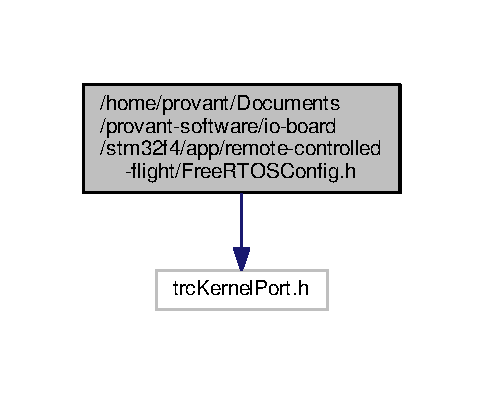
\includegraphics[width=232pt]{FreeRTOSConfig_8h__incl}
\end{center}
\end{figure}
\subsection*{Macros}
\begin{DoxyCompactItemize}
\item 
\#define \hyperlink{FreeRTOSConfig_8h_adde83486022745409c40605922b0bdd6}{config\+U\+S\+E\+\_\+\+P\+R\+E\+E\+M\+P\+T\+I\+ON}~1
\item 
\#define \hyperlink{FreeRTOSConfig_8h_ac637ae45863c19fa2e919db0ed49301f}{config\+U\+S\+E\+\_\+\+I\+D\+L\+E\+\_\+\+H\+O\+OK}~1
\item 
\#define \hyperlink{FreeRTOSConfig_8h_a23c5922c077106fad3f70b54d9071466}{config\+U\+S\+E\+\_\+\+T\+I\+C\+K\+\_\+\+H\+O\+OK}~0
\item 
\#define \hyperlink{FreeRTOSConfig_8h_aa68082df879e6fc96bcb9b26513639e7}{config\+C\+P\+U\+\_\+\+C\+L\+O\+C\+K\+\_\+\+HZ}~168000000
\item 
\#define \hyperlink{FreeRTOSConfig_8h_a2f0258dd1e3b877e5bc013be54c2db6a}{config\+T\+I\+C\+K\+\_\+\+R\+A\+T\+E\+\_\+\+HZ}~( ( port\+Tick\+Type ) 1000 )
\item 
\#define \hyperlink{FreeRTOSConfig_8h_a9a78f5ac61e6cb172dadf2a51f11db38}{config\+M\+A\+X\+\_\+\+P\+R\+I\+O\+R\+I\+T\+I\+ES}~( ( unsigned port\+B\+A\+S\+E\+\_\+\+T\+Y\+PE ) 5 )
\item 
\#define \hyperlink{FreeRTOSConfig_8h_a6c534a6cf8a00528fe0be42083484f9a}{config\+M\+I\+N\+I\+M\+A\+L\+\_\+\+S\+T\+A\+C\+K\+\_\+\+S\+I\+ZE}~1024
\item 
\#define \hyperlink{FreeRTOSConfig_8h_a9f213227674effff0122a75d94d87938}{config\+T\+O\+T\+A\+L\+\_\+\+H\+E\+A\+P\+\_\+\+S\+I\+ZE}~( ( size\+\_\+t ) ( 75 $\ast$ 1024 ) )
\item 
\#define \hyperlink{FreeRTOSConfig_8h_ac388dc4041aab6997348828eb27fc1a8}{config\+M\+A\+X\+\_\+\+T\+A\+S\+K\+\_\+\+N\+A\+M\+E\+\_\+\+L\+EN}~( 10 )
\item 
\#define \hyperlink{FreeRTOSConfig_8h_a27f5ee137dc9f125681a31f0b0a4b3be}{config\+U\+S\+E\+\_\+\+T\+R\+A\+C\+E\+\_\+\+F\+A\+C\+I\+L\+I\+TY}~1
\item 
\#define \hyperlink{FreeRTOSConfig_8h_aac311ed9b9e5ae4d2d9648b33a24acce}{config\+U\+S\+E\+\_\+16\+\_\+\+B\+I\+T\+\_\+\+T\+I\+C\+KS}~0
\item 
\#define \hyperlink{FreeRTOSConfig_8h_ad6a5061a742fee450ac455e4ad0f4b6c}{config\+I\+D\+L\+E\+\_\+\+S\+H\+O\+U\+L\+D\+\_\+\+Y\+I\+E\+LD}~1
\item 
\#define \hyperlink{FreeRTOSConfig_8h_a543bf3c79008974cc1d36bab51d94fbf}{config\+U\+S\+E\+\_\+\+M\+U\+T\+E\+X\+ES}~1
\item 
\#define \hyperlink{FreeRTOSConfig_8h_aa4b5138c4e42a180f0abd4f2455f90fb}{config\+Q\+U\+E\+U\+E\+\_\+\+R\+E\+G\+I\+S\+T\+R\+Y\+\_\+\+S\+I\+ZE}~8
\item 
\#define \hyperlink{FreeRTOSConfig_8h_a847511ee433494b1e32c90602c967ae7}{config\+C\+H\+E\+C\+K\+\_\+\+F\+O\+R\+\_\+\+S\+T\+A\+C\+K\+\_\+\+O\+V\+E\+R\+F\+L\+OW}~2
\item 
\#define \hyperlink{FreeRTOSConfig_8h_a9fe02d866cb1c4fbaa0c3de79f53d42d}{config\+U\+S\+E\+\_\+\+R\+E\+C\+U\+R\+S\+I\+V\+E\+\_\+\+M\+U\+T\+E\+X\+ES}~1
\item 
\#define \hyperlink{FreeRTOSConfig_8h_abdf48e7c9cf513f083aa9cbed0dd7cd7}{config\+U\+S\+E\+\_\+\+M\+A\+L\+L\+O\+C\+\_\+\+F\+A\+I\+L\+E\+D\+\_\+\+H\+O\+OK}~1
\item 
\#define \hyperlink{FreeRTOSConfig_8h_a2eb2a0baf886a7adab15b5735029434b}{config\+U\+S\+E\+\_\+\+A\+P\+P\+L\+I\+C\+A\+T\+I\+O\+N\+\_\+\+T\+A\+S\+K\+\_\+\+T\+AG}~0
\item 
\#define \hyperlink{FreeRTOSConfig_8h_a55778995203c57369d2fbfb10224943d}{config\+U\+S\+E\+\_\+\+C\+O\+U\+N\+T\+I\+N\+G\+\_\+\+S\+E\+M\+A\+P\+H\+O\+R\+ES}~1
\item 
\#define \hyperlink{FreeRTOSConfig_8h_ad8081822f3ebc7c917b63bd7bdd7bc58}{config\+G\+E\+N\+E\+R\+A\+T\+E\+\_\+\+R\+U\+N\+\_\+\+T\+I\+M\+E\+\_\+\+S\+T\+A\+TS}~0
\item 
\#define \hyperlink{FreeRTOSConfig_8h_a57990715eb06402474b8b47e1d562616}{config\+U\+S\+E\+\_\+\+C\+O\+\_\+\+R\+O\+U\+T\+I\+N\+ES}~0
\item 
\#define \hyperlink{FreeRTOSConfig_8h_ae8f3fd645e6e78dfeb8a6e874af6195a}{config\+M\+A\+X\+\_\+\+C\+O\+\_\+\+R\+O\+U\+T\+I\+N\+E\+\_\+\+P\+R\+I\+O\+R\+I\+T\+I\+ES}~( 2 )
\item 
\#define \hyperlink{FreeRTOSConfig_8h_ac342ae309b0c53828d2ecad3e6de355b}{config\+U\+S\+E\+\_\+\+T\+I\+M\+E\+RS}~1
\item 
\#define \hyperlink{FreeRTOSConfig_8h_a05c75ff9029ba3f0ab5bde9196f1e873}{config\+T\+I\+M\+E\+R\+\_\+\+T\+A\+S\+K\+\_\+\+P\+R\+I\+O\+R\+I\+TY}~( 2 )
\item 
\#define \hyperlink{FreeRTOSConfig_8h_abb9aa0f31c1f3b14a15083a3c6120918}{config\+T\+I\+M\+E\+R\+\_\+\+Q\+U\+E\+U\+E\+\_\+\+L\+E\+N\+G\+TH}~10
\item 
\#define \hyperlink{FreeRTOSConfig_8h_aed7c7ebcdee603583a55e8ce04e55841}{config\+T\+I\+M\+E\+R\+\_\+\+T\+A\+S\+K\+\_\+\+S\+T\+A\+C\+K\+\_\+\+D\+E\+P\+TH}~( \hyperlink{FreeRTOSConfig_8h_a6c534a6cf8a00528fe0be42083484f9a}{config\+M\+I\+N\+I\+M\+A\+L\+\_\+\+S\+T\+A\+C\+K\+\_\+\+S\+I\+ZE} $\ast$ 2 )
\item 
\#define \hyperlink{FreeRTOSConfig_8h_ad6858ac8aaf726007fd19752956ef1bd}{I\+N\+C\+L\+U\+D\+E\+\_\+v\+Task\+Priority\+Set}~1
\item 
\#define \hyperlink{FreeRTOSConfig_8h_a1279eb797355460aeeec06aa524e91df}{I\+N\+C\+L\+U\+D\+E\+\_\+ux\+Task\+Priority\+Get}~1
\item 
\#define \hyperlink{FreeRTOSConfig_8h_a5ae1434fdf995108dc749ff9329f53bd}{I\+N\+C\+L\+U\+D\+E\+\_\+v\+Task\+Delete}~1
\item 
\#define \hyperlink{FreeRTOSConfig_8h_a7ee138825e57f243c8ee5fd4207b9e26}{I\+N\+C\+L\+U\+D\+E\+\_\+v\+Task\+Clean\+Up\+Resources}~1
\item 
\#define \hyperlink{FreeRTOSConfig_8h_aef8fbb97819ad3d962f334ac298206d1}{I\+N\+C\+L\+U\+D\+E\+\_\+v\+Task\+Suspend}~1
\item 
\#define \hyperlink{FreeRTOSConfig_8h_ae8459bfd5b428319bb10de9f504a53aa}{I\+N\+C\+L\+U\+D\+E\+\_\+v\+Task\+Delay\+Until}~1
\item 
\#define \hyperlink{FreeRTOSConfig_8h_a24361a6eb816a965f1ee4e2e08e364f8}{I\+N\+C\+L\+U\+D\+E\+\_\+v\+Task\+Delay}~1
\item 
\#define \hyperlink{FreeRTOSConfig_8h_a5796db11ec6f9aa38d017d2ac393c5ba}{config\+P\+R\+I\+O\+\_\+\+B\+I\+TS}~4        /$\ast$ 15 priority levels $\ast$/
\item 
\#define \hyperlink{FreeRTOSConfig_8h_a10da20f180ec9bd131b0052a802dbc39}{config\+L\+I\+B\+R\+A\+R\+Y\+\_\+\+L\+O\+W\+E\+S\+T\+\_\+\+I\+N\+T\+E\+R\+R\+U\+P\+T\+\_\+\+P\+R\+I\+O\+R\+I\+TY}~0xf
\item 
\#define \hyperlink{FreeRTOSConfig_8h_a2254bd235d882be3061bcad0b1e8be98}{config\+L\+I\+B\+R\+A\+R\+Y\+\_\+\+M\+A\+X\+\_\+\+S\+Y\+S\+C\+A\+L\+L\+\_\+\+I\+N\+T\+E\+R\+R\+U\+P\+T\+\_\+\+P\+R\+I\+O\+R\+I\+TY}~5
\item 
\#define \hyperlink{FreeRTOSConfig_8h_ac42cff506ad61d4174fa23e952e3225e}{config\+K\+E\+R\+N\+E\+L\+\_\+\+I\+N\+T\+E\+R\+R\+U\+P\+T\+\_\+\+P\+R\+I\+O\+R\+I\+TY}~( \hyperlink{FreeRTOSConfig_8h_a10da20f180ec9bd131b0052a802dbc39}{config\+L\+I\+B\+R\+A\+R\+Y\+\_\+\+L\+O\+W\+E\+S\+T\+\_\+\+I\+N\+T\+E\+R\+R\+U\+P\+T\+\_\+\+P\+R\+I\+O\+R\+I\+TY} $<$$<$ (8 -\/ \hyperlink{FreeRTOSConfig_8h_a5796db11ec6f9aa38d017d2ac393c5ba}{config\+P\+R\+I\+O\+\_\+\+B\+I\+TS}) )
\item 
\#define \hyperlink{FreeRTOSConfig_8h_a54bfc31c410ee452577a25a4552c3704}{config\+M\+A\+X\+\_\+\+S\+Y\+S\+C\+A\+L\+L\+\_\+\+I\+N\+T\+E\+R\+R\+U\+P\+T\+\_\+\+P\+R\+I\+O\+R\+I\+TY}~( \hyperlink{FreeRTOSConfig_8h_a2254bd235d882be3061bcad0b1e8be98}{config\+L\+I\+B\+R\+A\+R\+Y\+\_\+\+M\+A\+X\+\_\+\+S\+Y\+S\+C\+A\+L\+L\+\_\+\+I\+N\+T\+E\+R\+R\+U\+P\+T\+\_\+\+P\+R\+I\+O\+R\+I\+TY} $<$$<$ (8 -\/ \hyperlink{FreeRTOSConfig_8h_a5796db11ec6f9aa38d017d2ac393c5ba}{config\+P\+R\+I\+O\+\_\+\+B\+I\+TS}) )
\item 
\#define \hyperlink{FreeRTOSConfig_8h_a228c70cd48927d6ab730ed1a6dfbe35f}{config\+A\+S\+S\+E\+RT}(x)~if( ( x ) == 0 ) \{ task\+D\+I\+S\+A\+B\+L\+E\+\_\+\+I\+N\+T\+E\+R\+R\+U\+P\+TS(); for( ;; ); \}
\item 
\#define \hyperlink{FreeRTOSConfig_8h_ad43047b3ea0a146673e30637488bf754}{v\+Port\+S\+V\+C\+Handler}~S\+V\+C\+\_\+\+Handler
\item 
\#define \hyperlink{FreeRTOSConfig_8h_a6f30022da7d797dd31f1b8a11cae9a35}{x\+Port\+Pend\+S\+V\+Handler}~Pend\+S\+V\+\_\+\+Handler
\item 
\#define \hyperlink{FreeRTOSConfig_8h_ae42e6318b5d564e44f97f8c765859448}{x\+Port\+Sys\+Tick\+Handler}~Sys\+Tick\+\_\+\+Handler
\item 
\#define \hyperlink{FreeRTOSConfig_8h_a27f5ee137dc9f125681a31f0b0a4b3be}{config\+U\+S\+E\+\_\+\+T\+R\+A\+C\+E\+\_\+\+F\+A\+C\+I\+L\+I\+TY}~1
\end{DoxyCompactItemize}


\subsection{Macro Definition Documentation}
\index{Free\+R\+T\+O\+S\+Config.\+h@{Free\+R\+T\+O\+S\+Config.\+h}!config\+A\+S\+S\+E\+RT@{config\+A\+S\+S\+E\+RT}}
\index{config\+A\+S\+S\+E\+RT@{config\+A\+S\+S\+E\+RT}!Free\+R\+T\+O\+S\+Config.\+h@{Free\+R\+T\+O\+S\+Config.\+h}}
\subsubsection[{\texorpdfstring{config\+A\+S\+S\+E\+RT}{configASSERT}}]{\setlength{\rightskip}{0pt plus 5cm}\#define config\+A\+S\+S\+E\+RT(
\begin{DoxyParamCaption}
\item[{}]{x}
\end{DoxyParamCaption}
)~if( ( x ) == 0 ) \{ task\+D\+I\+S\+A\+B\+L\+E\+\_\+\+I\+N\+T\+E\+R\+R\+U\+P\+TS(); for( ;; ); \}}\hypertarget{FreeRTOSConfig_8h_a228c70cd48927d6ab730ed1a6dfbe35f}{}\label{FreeRTOSConfig_8h_a228c70cd48927d6ab730ed1a6dfbe35f}


Definition at line 155 of file Free\+R\+T\+O\+S\+Config.\+h.

\index{Free\+R\+T\+O\+S\+Config.\+h@{Free\+R\+T\+O\+S\+Config.\+h}!config\+C\+H\+E\+C\+K\+\_\+\+F\+O\+R\+\_\+\+S\+T\+A\+C\+K\+\_\+\+O\+V\+E\+R\+F\+L\+OW@{config\+C\+H\+E\+C\+K\+\_\+\+F\+O\+R\+\_\+\+S\+T\+A\+C\+K\+\_\+\+O\+V\+E\+R\+F\+L\+OW}}
\index{config\+C\+H\+E\+C\+K\+\_\+\+F\+O\+R\+\_\+\+S\+T\+A\+C\+K\+\_\+\+O\+V\+E\+R\+F\+L\+OW@{config\+C\+H\+E\+C\+K\+\_\+\+F\+O\+R\+\_\+\+S\+T\+A\+C\+K\+\_\+\+O\+V\+E\+R\+F\+L\+OW}!Free\+R\+T\+O\+S\+Config.\+h@{Free\+R\+T\+O\+S\+Config.\+h}}
\subsubsection[{\texorpdfstring{config\+C\+H\+E\+C\+K\+\_\+\+F\+O\+R\+\_\+\+S\+T\+A\+C\+K\+\_\+\+O\+V\+E\+R\+F\+L\+OW}{configCHECK_FOR_STACK_OVERFLOW}}]{\setlength{\rightskip}{0pt plus 5cm}\#define config\+C\+H\+E\+C\+K\+\_\+\+F\+O\+R\+\_\+\+S\+T\+A\+C\+K\+\_\+\+O\+V\+E\+R\+F\+L\+OW~2}\hypertarget{FreeRTOSConfig_8h_a847511ee433494b1e32c90602c967ae7}{}\label{FreeRTOSConfig_8h_a847511ee433494b1e32c90602c967ae7}


Definition at line 101 of file Free\+R\+T\+O\+S\+Config.\+h.

\index{Free\+R\+T\+O\+S\+Config.\+h@{Free\+R\+T\+O\+S\+Config.\+h}!config\+C\+P\+U\+\_\+\+C\+L\+O\+C\+K\+\_\+\+HZ@{config\+C\+P\+U\+\_\+\+C\+L\+O\+C\+K\+\_\+\+HZ}}
\index{config\+C\+P\+U\+\_\+\+C\+L\+O\+C\+K\+\_\+\+HZ@{config\+C\+P\+U\+\_\+\+C\+L\+O\+C\+K\+\_\+\+HZ}!Free\+R\+T\+O\+S\+Config.\+h@{Free\+R\+T\+O\+S\+Config.\+h}}
\subsubsection[{\texorpdfstring{config\+C\+P\+U\+\_\+\+C\+L\+O\+C\+K\+\_\+\+HZ}{configCPU_CLOCK_HZ}}]{\setlength{\rightskip}{0pt plus 5cm}\#define config\+C\+P\+U\+\_\+\+C\+L\+O\+C\+K\+\_\+\+HZ~168000000}\hypertarget{FreeRTOSConfig_8h_aa68082df879e6fc96bcb9b26513639e7}{}\label{FreeRTOSConfig_8h_aa68082df879e6fc96bcb9b26513639e7}


Definition at line 90 of file Free\+R\+T\+O\+S\+Config.\+h.

\index{Free\+R\+T\+O\+S\+Config.\+h@{Free\+R\+T\+O\+S\+Config.\+h}!config\+G\+E\+N\+E\+R\+A\+T\+E\+\_\+\+R\+U\+N\+\_\+\+T\+I\+M\+E\+\_\+\+S\+T\+A\+TS@{config\+G\+E\+N\+E\+R\+A\+T\+E\+\_\+\+R\+U\+N\+\_\+\+T\+I\+M\+E\+\_\+\+S\+T\+A\+TS}}
\index{config\+G\+E\+N\+E\+R\+A\+T\+E\+\_\+\+R\+U\+N\+\_\+\+T\+I\+M\+E\+\_\+\+S\+T\+A\+TS@{config\+G\+E\+N\+E\+R\+A\+T\+E\+\_\+\+R\+U\+N\+\_\+\+T\+I\+M\+E\+\_\+\+S\+T\+A\+TS}!Free\+R\+T\+O\+S\+Config.\+h@{Free\+R\+T\+O\+S\+Config.\+h}}
\subsubsection[{\texorpdfstring{config\+G\+E\+N\+E\+R\+A\+T\+E\+\_\+\+R\+U\+N\+\_\+\+T\+I\+M\+E\+\_\+\+S\+T\+A\+TS}{configGENERATE_RUN_TIME_STATS}}]{\setlength{\rightskip}{0pt plus 5cm}\#define config\+G\+E\+N\+E\+R\+A\+T\+E\+\_\+\+R\+U\+N\+\_\+\+T\+I\+M\+E\+\_\+\+S\+T\+A\+TS~0}\hypertarget{FreeRTOSConfig_8h_ad8081822f3ebc7c917b63bd7bdd7bc58}{}\label{FreeRTOSConfig_8h_ad8081822f3ebc7c917b63bd7bdd7bc58}


Definition at line 106 of file Free\+R\+T\+O\+S\+Config.\+h.

\index{Free\+R\+T\+O\+S\+Config.\+h@{Free\+R\+T\+O\+S\+Config.\+h}!config\+I\+D\+L\+E\+\_\+\+S\+H\+O\+U\+L\+D\+\_\+\+Y\+I\+E\+LD@{config\+I\+D\+L\+E\+\_\+\+S\+H\+O\+U\+L\+D\+\_\+\+Y\+I\+E\+LD}}
\index{config\+I\+D\+L\+E\+\_\+\+S\+H\+O\+U\+L\+D\+\_\+\+Y\+I\+E\+LD@{config\+I\+D\+L\+E\+\_\+\+S\+H\+O\+U\+L\+D\+\_\+\+Y\+I\+E\+LD}!Free\+R\+T\+O\+S\+Config.\+h@{Free\+R\+T\+O\+S\+Config.\+h}}
\subsubsection[{\texorpdfstring{config\+I\+D\+L\+E\+\_\+\+S\+H\+O\+U\+L\+D\+\_\+\+Y\+I\+E\+LD}{configIDLE_SHOULD_YIELD}}]{\setlength{\rightskip}{0pt plus 5cm}\#define config\+I\+D\+L\+E\+\_\+\+S\+H\+O\+U\+L\+D\+\_\+\+Y\+I\+E\+LD~1}\hypertarget{FreeRTOSConfig_8h_ad6a5061a742fee450ac455e4ad0f4b6c}{}\label{FreeRTOSConfig_8h_ad6a5061a742fee450ac455e4ad0f4b6c}


Definition at line 98 of file Free\+R\+T\+O\+S\+Config.\+h.

\index{Free\+R\+T\+O\+S\+Config.\+h@{Free\+R\+T\+O\+S\+Config.\+h}!config\+K\+E\+R\+N\+E\+L\+\_\+\+I\+N\+T\+E\+R\+R\+U\+P\+T\+\_\+\+P\+R\+I\+O\+R\+I\+TY@{config\+K\+E\+R\+N\+E\+L\+\_\+\+I\+N\+T\+E\+R\+R\+U\+P\+T\+\_\+\+P\+R\+I\+O\+R\+I\+TY}}
\index{config\+K\+E\+R\+N\+E\+L\+\_\+\+I\+N\+T\+E\+R\+R\+U\+P\+T\+\_\+\+P\+R\+I\+O\+R\+I\+TY@{config\+K\+E\+R\+N\+E\+L\+\_\+\+I\+N\+T\+E\+R\+R\+U\+P\+T\+\_\+\+P\+R\+I\+O\+R\+I\+TY}!Free\+R\+T\+O\+S\+Config.\+h@{Free\+R\+T\+O\+S\+Config.\+h}}
\subsubsection[{\texorpdfstring{config\+K\+E\+R\+N\+E\+L\+\_\+\+I\+N\+T\+E\+R\+R\+U\+P\+T\+\_\+\+P\+R\+I\+O\+R\+I\+TY}{configKERNEL_INTERRUPT_PRIORITY}}]{\setlength{\rightskip}{0pt plus 5cm}\#define config\+K\+E\+R\+N\+E\+L\+\_\+\+I\+N\+T\+E\+R\+R\+U\+P\+T\+\_\+\+P\+R\+I\+O\+R\+I\+TY~( {\bf config\+L\+I\+B\+R\+A\+R\+Y\+\_\+\+L\+O\+W\+E\+S\+T\+\_\+\+I\+N\+T\+E\+R\+R\+U\+P\+T\+\_\+\+P\+R\+I\+O\+R\+I\+TY} $<$$<$ (8 -\/ {\bf config\+P\+R\+I\+O\+\_\+\+B\+I\+TS}) )}\hypertarget{FreeRTOSConfig_8h_ac42cff506ad61d4174fa23e952e3225e}{}\label{FreeRTOSConfig_8h_ac42cff506ad61d4174fa23e952e3225e}


Definition at line 148 of file Free\+R\+T\+O\+S\+Config.\+h.

\index{Free\+R\+T\+O\+S\+Config.\+h@{Free\+R\+T\+O\+S\+Config.\+h}!config\+L\+I\+B\+R\+A\+R\+Y\+\_\+\+L\+O\+W\+E\+S\+T\+\_\+\+I\+N\+T\+E\+R\+R\+U\+P\+T\+\_\+\+P\+R\+I\+O\+R\+I\+TY@{config\+L\+I\+B\+R\+A\+R\+Y\+\_\+\+L\+O\+W\+E\+S\+T\+\_\+\+I\+N\+T\+E\+R\+R\+U\+P\+T\+\_\+\+P\+R\+I\+O\+R\+I\+TY}}
\index{config\+L\+I\+B\+R\+A\+R\+Y\+\_\+\+L\+O\+W\+E\+S\+T\+\_\+\+I\+N\+T\+E\+R\+R\+U\+P\+T\+\_\+\+P\+R\+I\+O\+R\+I\+TY@{config\+L\+I\+B\+R\+A\+R\+Y\+\_\+\+L\+O\+W\+E\+S\+T\+\_\+\+I\+N\+T\+E\+R\+R\+U\+P\+T\+\_\+\+P\+R\+I\+O\+R\+I\+TY}!Free\+R\+T\+O\+S\+Config.\+h@{Free\+R\+T\+O\+S\+Config.\+h}}
\subsubsection[{\texorpdfstring{config\+L\+I\+B\+R\+A\+R\+Y\+\_\+\+L\+O\+W\+E\+S\+T\+\_\+\+I\+N\+T\+E\+R\+R\+U\+P\+T\+\_\+\+P\+R\+I\+O\+R\+I\+TY}{configLIBRARY_LOWEST_INTERRUPT_PRIORITY}}]{\setlength{\rightskip}{0pt plus 5cm}\#define config\+L\+I\+B\+R\+A\+R\+Y\+\_\+\+L\+O\+W\+E\+S\+T\+\_\+\+I\+N\+T\+E\+R\+R\+U\+P\+T\+\_\+\+P\+R\+I\+O\+R\+I\+TY~0xf}\hypertarget{FreeRTOSConfig_8h_a10da20f180ec9bd131b0052a802dbc39}{}\label{FreeRTOSConfig_8h_a10da20f180ec9bd131b0052a802dbc39}


Definition at line 138 of file Free\+R\+T\+O\+S\+Config.\+h.

\index{Free\+R\+T\+O\+S\+Config.\+h@{Free\+R\+T\+O\+S\+Config.\+h}!config\+L\+I\+B\+R\+A\+R\+Y\+\_\+\+M\+A\+X\+\_\+\+S\+Y\+S\+C\+A\+L\+L\+\_\+\+I\+N\+T\+E\+R\+R\+U\+P\+T\+\_\+\+P\+R\+I\+O\+R\+I\+TY@{config\+L\+I\+B\+R\+A\+R\+Y\+\_\+\+M\+A\+X\+\_\+\+S\+Y\+S\+C\+A\+L\+L\+\_\+\+I\+N\+T\+E\+R\+R\+U\+P\+T\+\_\+\+P\+R\+I\+O\+R\+I\+TY}}
\index{config\+L\+I\+B\+R\+A\+R\+Y\+\_\+\+M\+A\+X\+\_\+\+S\+Y\+S\+C\+A\+L\+L\+\_\+\+I\+N\+T\+E\+R\+R\+U\+P\+T\+\_\+\+P\+R\+I\+O\+R\+I\+TY@{config\+L\+I\+B\+R\+A\+R\+Y\+\_\+\+M\+A\+X\+\_\+\+S\+Y\+S\+C\+A\+L\+L\+\_\+\+I\+N\+T\+E\+R\+R\+U\+P\+T\+\_\+\+P\+R\+I\+O\+R\+I\+TY}!Free\+R\+T\+O\+S\+Config.\+h@{Free\+R\+T\+O\+S\+Config.\+h}}
\subsubsection[{\texorpdfstring{config\+L\+I\+B\+R\+A\+R\+Y\+\_\+\+M\+A\+X\+\_\+\+S\+Y\+S\+C\+A\+L\+L\+\_\+\+I\+N\+T\+E\+R\+R\+U\+P\+T\+\_\+\+P\+R\+I\+O\+R\+I\+TY}{configLIBRARY_MAX_SYSCALL_INTERRUPT_PRIORITY}}]{\setlength{\rightskip}{0pt plus 5cm}\#define config\+L\+I\+B\+R\+A\+R\+Y\+\_\+\+M\+A\+X\+\_\+\+S\+Y\+S\+C\+A\+L\+L\+\_\+\+I\+N\+T\+E\+R\+R\+U\+P\+T\+\_\+\+P\+R\+I\+O\+R\+I\+TY~5}\hypertarget{FreeRTOSConfig_8h_a2254bd235d882be3061bcad0b1e8be98}{}\label{FreeRTOSConfig_8h_a2254bd235d882be3061bcad0b1e8be98}


Definition at line 144 of file Free\+R\+T\+O\+S\+Config.\+h.

\index{Free\+R\+T\+O\+S\+Config.\+h@{Free\+R\+T\+O\+S\+Config.\+h}!config\+M\+A\+X\+\_\+\+C\+O\+\_\+\+R\+O\+U\+T\+I\+N\+E\+\_\+\+P\+R\+I\+O\+R\+I\+T\+I\+ES@{config\+M\+A\+X\+\_\+\+C\+O\+\_\+\+R\+O\+U\+T\+I\+N\+E\+\_\+\+P\+R\+I\+O\+R\+I\+T\+I\+ES}}
\index{config\+M\+A\+X\+\_\+\+C\+O\+\_\+\+R\+O\+U\+T\+I\+N\+E\+\_\+\+P\+R\+I\+O\+R\+I\+T\+I\+ES@{config\+M\+A\+X\+\_\+\+C\+O\+\_\+\+R\+O\+U\+T\+I\+N\+E\+\_\+\+P\+R\+I\+O\+R\+I\+T\+I\+ES}!Free\+R\+T\+O\+S\+Config.\+h@{Free\+R\+T\+O\+S\+Config.\+h}}
\subsubsection[{\texorpdfstring{config\+M\+A\+X\+\_\+\+C\+O\+\_\+\+R\+O\+U\+T\+I\+N\+E\+\_\+\+P\+R\+I\+O\+R\+I\+T\+I\+ES}{configMAX_CO_ROUTINE_PRIORITIES}}]{\setlength{\rightskip}{0pt plus 5cm}\#define config\+M\+A\+X\+\_\+\+C\+O\+\_\+\+R\+O\+U\+T\+I\+N\+E\+\_\+\+P\+R\+I\+O\+R\+I\+T\+I\+ES~( 2 )}\hypertarget{FreeRTOSConfig_8h_ae8f3fd645e6e78dfeb8a6e874af6195a}{}\label{FreeRTOSConfig_8h_ae8f3fd645e6e78dfeb8a6e874af6195a}


Definition at line 110 of file Free\+R\+T\+O\+S\+Config.\+h.

\index{Free\+R\+T\+O\+S\+Config.\+h@{Free\+R\+T\+O\+S\+Config.\+h}!config\+M\+A\+X\+\_\+\+P\+R\+I\+O\+R\+I\+T\+I\+ES@{config\+M\+A\+X\+\_\+\+P\+R\+I\+O\+R\+I\+T\+I\+ES}}
\index{config\+M\+A\+X\+\_\+\+P\+R\+I\+O\+R\+I\+T\+I\+ES@{config\+M\+A\+X\+\_\+\+P\+R\+I\+O\+R\+I\+T\+I\+ES}!Free\+R\+T\+O\+S\+Config.\+h@{Free\+R\+T\+O\+S\+Config.\+h}}
\subsubsection[{\texorpdfstring{config\+M\+A\+X\+\_\+\+P\+R\+I\+O\+R\+I\+T\+I\+ES}{configMAX_PRIORITIES}}]{\setlength{\rightskip}{0pt plus 5cm}\#define config\+M\+A\+X\+\_\+\+P\+R\+I\+O\+R\+I\+T\+I\+ES~( ( unsigned port\+B\+A\+S\+E\+\_\+\+T\+Y\+PE ) 5 )}\hypertarget{FreeRTOSConfig_8h_a9a78f5ac61e6cb172dadf2a51f11db38}{}\label{FreeRTOSConfig_8h_a9a78f5ac61e6cb172dadf2a51f11db38}


Definition at line 92 of file Free\+R\+T\+O\+S\+Config.\+h.

\index{Free\+R\+T\+O\+S\+Config.\+h@{Free\+R\+T\+O\+S\+Config.\+h}!config\+M\+A\+X\+\_\+\+S\+Y\+S\+C\+A\+L\+L\+\_\+\+I\+N\+T\+E\+R\+R\+U\+P\+T\+\_\+\+P\+R\+I\+O\+R\+I\+TY@{config\+M\+A\+X\+\_\+\+S\+Y\+S\+C\+A\+L\+L\+\_\+\+I\+N\+T\+E\+R\+R\+U\+P\+T\+\_\+\+P\+R\+I\+O\+R\+I\+TY}}
\index{config\+M\+A\+X\+\_\+\+S\+Y\+S\+C\+A\+L\+L\+\_\+\+I\+N\+T\+E\+R\+R\+U\+P\+T\+\_\+\+P\+R\+I\+O\+R\+I\+TY@{config\+M\+A\+X\+\_\+\+S\+Y\+S\+C\+A\+L\+L\+\_\+\+I\+N\+T\+E\+R\+R\+U\+P\+T\+\_\+\+P\+R\+I\+O\+R\+I\+TY}!Free\+R\+T\+O\+S\+Config.\+h@{Free\+R\+T\+O\+S\+Config.\+h}}
\subsubsection[{\texorpdfstring{config\+M\+A\+X\+\_\+\+S\+Y\+S\+C\+A\+L\+L\+\_\+\+I\+N\+T\+E\+R\+R\+U\+P\+T\+\_\+\+P\+R\+I\+O\+R\+I\+TY}{configMAX_SYSCALL_INTERRUPT_PRIORITY}}]{\setlength{\rightskip}{0pt plus 5cm}\#define config\+M\+A\+X\+\_\+\+S\+Y\+S\+C\+A\+L\+L\+\_\+\+I\+N\+T\+E\+R\+R\+U\+P\+T\+\_\+\+P\+R\+I\+O\+R\+I\+TY~( {\bf config\+L\+I\+B\+R\+A\+R\+Y\+\_\+\+M\+A\+X\+\_\+\+S\+Y\+S\+C\+A\+L\+L\+\_\+\+I\+N\+T\+E\+R\+R\+U\+P\+T\+\_\+\+P\+R\+I\+O\+R\+I\+TY} $<$$<$ (8 -\/ {\bf config\+P\+R\+I\+O\+\_\+\+B\+I\+TS}) )}\hypertarget{FreeRTOSConfig_8h_a54bfc31c410ee452577a25a4552c3704}{}\label{FreeRTOSConfig_8h_a54bfc31c410ee452577a25a4552c3704}


Definition at line 151 of file Free\+R\+T\+O\+S\+Config.\+h.

\index{Free\+R\+T\+O\+S\+Config.\+h@{Free\+R\+T\+O\+S\+Config.\+h}!config\+M\+A\+X\+\_\+\+T\+A\+S\+K\+\_\+\+N\+A\+M\+E\+\_\+\+L\+EN@{config\+M\+A\+X\+\_\+\+T\+A\+S\+K\+\_\+\+N\+A\+M\+E\+\_\+\+L\+EN}}
\index{config\+M\+A\+X\+\_\+\+T\+A\+S\+K\+\_\+\+N\+A\+M\+E\+\_\+\+L\+EN@{config\+M\+A\+X\+\_\+\+T\+A\+S\+K\+\_\+\+N\+A\+M\+E\+\_\+\+L\+EN}!Free\+R\+T\+O\+S\+Config.\+h@{Free\+R\+T\+O\+S\+Config.\+h}}
\subsubsection[{\texorpdfstring{config\+M\+A\+X\+\_\+\+T\+A\+S\+K\+\_\+\+N\+A\+M\+E\+\_\+\+L\+EN}{configMAX_TASK_NAME_LEN}}]{\setlength{\rightskip}{0pt plus 5cm}\#define config\+M\+A\+X\+\_\+\+T\+A\+S\+K\+\_\+\+N\+A\+M\+E\+\_\+\+L\+EN~( 10 )}\hypertarget{FreeRTOSConfig_8h_ac388dc4041aab6997348828eb27fc1a8}{}\label{FreeRTOSConfig_8h_ac388dc4041aab6997348828eb27fc1a8}


Definition at line 95 of file Free\+R\+T\+O\+S\+Config.\+h.

\index{Free\+R\+T\+O\+S\+Config.\+h@{Free\+R\+T\+O\+S\+Config.\+h}!config\+M\+I\+N\+I\+M\+A\+L\+\_\+\+S\+T\+A\+C\+K\+\_\+\+S\+I\+ZE@{config\+M\+I\+N\+I\+M\+A\+L\+\_\+\+S\+T\+A\+C\+K\+\_\+\+S\+I\+ZE}}
\index{config\+M\+I\+N\+I\+M\+A\+L\+\_\+\+S\+T\+A\+C\+K\+\_\+\+S\+I\+ZE@{config\+M\+I\+N\+I\+M\+A\+L\+\_\+\+S\+T\+A\+C\+K\+\_\+\+S\+I\+ZE}!Free\+R\+T\+O\+S\+Config.\+h@{Free\+R\+T\+O\+S\+Config.\+h}}
\subsubsection[{\texorpdfstring{config\+M\+I\+N\+I\+M\+A\+L\+\_\+\+S\+T\+A\+C\+K\+\_\+\+S\+I\+ZE}{configMINIMAL_STACK_SIZE}}]{\setlength{\rightskip}{0pt plus 5cm}\#define config\+M\+I\+N\+I\+M\+A\+L\+\_\+\+S\+T\+A\+C\+K\+\_\+\+S\+I\+ZE~1024}\hypertarget{FreeRTOSConfig_8h_a6c534a6cf8a00528fe0be42083484f9a}{}\label{FreeRTOSConfig_8h_a6c534a6cf8a00528fe0be42083484f9a}


Definition at line 93 of file Free\+R\+T\+O\+S\+Config.\+h.

\index{Free\+R\+T\+O\+S\+Config.\+h@{Free\+R\+T\+O\+S\+Config.\+h}!config\+P\+R\+I\+O\+\_\+\+B\+I\+TS@{config\+P\+R\+I\+O\+\_\+\+B\+I\+TS}}
\index{config\+P\+R\+I\+O\+\_\+\+B\+I\+TS@{config\+P\+R\+I\+O\+\_\+\+B\+I\+TS}!Free\+R\+T\+O\+S\+Config.\+h@{Free\+R\+T\+O\+S\+Config.\+h}}
\subsubsection[{\texorpdfstring{config\+P\+R\+I\+O\+\_\+\+B\+I\+TS}{configPRIO_BITS}}]{\setlength{\rightskip}{0pt plus 5cm}\#define config\+P\+R\+I\+O\+\_\+\+B\+I\+TS~4        /$\ast$ 15 priority levels $\ast$/}\hypertarget{FreeRTOSConfig_8h_a5796db11ec6f9aa38d017d2ac393c5ba}{}\label{FreeRTOSConfig_8h_a5796db11ec6f9aa38d017d2ac393c5ba}


Definition at line 133 of file Free\+R\+T\+O\+S\+Config.\+h.

\index{Free\+R\+T\+O\+S\+Config.\+h@{Free\+R\+T\+O\+S\+Config.\+h}!config\+Q\+U\+E\+U\+E\+\_\+\+R\+E\+G\+I\+S\+T\+R\+Y\+\_\+\+S\+I\+ZE@{config\+Q\+U\+E\+U\+E\+\_\+\+R\+E\+G\+I\+S\+T\+R\+Y\+\_\+\+S\+I\+ZE}}
\index{config\+Q\+U\+E\+U\+E\+\_\+\+R\+E\+G\+I\+S\+T\+R\+Y\+\_\+\+S\+I\+ZE@{config\+Q\+U\+E\+U\+E\+\_\+\+R\+E\+G\+I\+S\+T\+R\+Y\+\_\+\+S\+I\+ZE}!Free\+R\+T\+O\+S\+Config.\+h@{Free\+R\+T\+O\+S\+Config.\+h}}
\subsubsection[{\texorpdfstring{config\+Q\+U\+E\+U\+E\+\_\+\+R\+E\+G\+I\+S\+T\+R\+Y\+\_\+\+S\+I\+ZE}{configQUEUE_REGISTRY_SIZE}}]{\setlength{\rightskip}{0pt plus 5cm}\#define config\+Q\+U\+E\+U\+E\+\_\+\+R\+E\+G\+I\+S\+T\+R\+Y\+\_\+\+S\+I\+ZE~8}\hypertarget{FreeRTOSConfig_8h_aa4b5138c4e42a180f0abd4f2455f90fb}{}\label{FreeRTOSConfig_8h_aa4b5138c4e42a180f0abd4f2455f90fb}


Definition at line 100 of file Free\+R\+T\+O\+S\+Config.\+h.

\index{Free\+R\+T\+O\+S\+Config.\+h@{Free\+R\+T\+O\+S\+Config.\+h}!config\+T\+I\+C\+K\+\_\+\+R\+A\+T\+E\+\_\+\+HZ@{config\+T\+I\+C\+K\+\_\+\+R\+A\+T\+E\+\_\+\+HZ}}
\index{config\+T\+I\+C\+K\+\_\+\+R\+A\+T\+E\+\_\+\+HZ@{config\+T\+I\+C\+K\+\_\+\+R\+A\+T\+E\+\_\+\+HZ}!Free\+R\+T\+O\+S\+Config.\+h@{Free\+R\+T\+O\+S\+Config.\+h}}
\subsubsection[{\texorpdfstring{config\+T\+I\+C\+K\+\_\+\+R\+A\+T\+E\+\_\+\+HZ}{configTICK_RATE_HZ}}]{\setlength{\rightskip}{0pt plus 5cm}\#define config\+T\+I\+C\+K\+\_\+\+R\+A\+T\+E\+\_\+\+HZ~( ( port\+Tick\+Type ) 1000 )}\hypertarget{FreeRTOSConfig_8h_a2f0258dd1e3b877e5bc013be54c2db6a}{}\label{FreeRTOSConfig_8h_a2f0258dd1e3b877e5bc013be54c2db6a}


Definition at line 91 of file Free\+R\+T\+O\+S\+Config.\+h.

\index{Free\+R\+T\+O\+S\+Config.\+h@{Free\+R\+T\+O\+S\+Config.\+h}!config\+T\+I\+M\+E\+R\+\_\+\+Q\+U\+E\+U\+E\+\_\+\+L\+E\+N\+G\+TH@{config\+T\+I\+M\+E\+R\+\_\+\+Q\+U\+E\+U\+E\+\_\+\+L\+E\+N\+G\+TH}}
\index{config\+T\+I\+M\+E\+R\+\_\+\+Q\+U\+E\+U\+E\+\_\+\+L\+E\+N\+G\+TH@{config\+T\+I\+M\+E\+R\+\_\+\+Q\+U\+E\+U\+E\+\_\+\+L\+E\+N\+G\+TH}!Free\+R\+T\+O\+S\+Config.\+h@{Free\+R\+T\+O\+S\+Config.\+h}}
\subsubsection[{\texorpdfstring{config\+T\+I\+M\+E\+R\+\_\+\+Q\+U\+E\+U\+E\+\_\+\+L\+E\+N\+G\+TH}{configTIMER_QUEUE_LENGTH}}]{\setlength{\rightskip}{0pt plus 5cm}\#define config\+T\+I\+M\+E\+R\+\_\+\+Q\+U\+E\+U\+E\+\_\+\+L\+E\+N\+G\+TH~10}\hypertarget{FreeRTOSConfig_8h_abb9aa0f31c1f3b14a15083a3c6120918}{}\label{FreeRTOSConfig_8h_abb9aa0f31c1f3b14a15083a3c6120918}


Definition at line 115 of file Free\+R\+T\+O\+S\+Config.\+h.

\index{Free\+R\+T\+O\+S\+Config.\+h@{Free\+R\+T\+O\+S\+Config.\+h}!config\+T\+I\+M\+E\+R\+\_\+\+T\+A\+S\+K\+\_\+\+P\+R\+I\+O\+R\+I\+TY@{config\+T\+I\+M\+E\+R\+\_\+\+T\+A\+S\+K\+\_\+\+P\+R\+I\+O\+R\+I\+TY}}
\index{config\+T\+I\+M\+E\+R\+\_\+\+T\+A\+S\+K\+\_\+\+P\+R\+I\+O\+R\+I\+TY@{config\+T\+I\+M\+E\+R\+\_\+\+T\+A\+S\+K\+\_\+\+P\+R\+I\+O\+R\+I\+TY}!Free\+R\+T\+O\+S\+Config.\+h@{Free\+R\+T\+O\+S\+Config.\+h}}
\subsubsection[{\texorpdfstring{config\+T\+I\+M\+E\+R\+\_\+\+T\+A\+S\+K\+\_\+\+P\+R\+I\+O\+R\+I\+TY}{configTIMER_TASK_PRIORITY}}]{\setlength{\rightskip}{0pt plus 5cm}\#define config\+T\+I\+M\+E\+R\+\_\+\+T\+A\+S\+K\+\_\+\+P\+R\+I\+O\+R\+I\+TY~( 2 )}\hypertarget{FreeRTOSConfig_8h_a05c75ff9029ba3f0ab5bde9196f1e873}{}\label{FreeRTOSConfig_8h_a05c75ff9029ba3f0ab5bde9196f1e873}


Definition at line 114 of file Free\+R\+T\+O\+S\+Config.\+h.

\index{Free\+R\+T\+O\+S\+Config.\+h@{Free\+R\+T\+O\+S\+Config.\+h}!config\+T\+I\+M\+E\+R\+\_\+\+T\+A\+S\+K\+\_\+\+S\+T\+A\+C\+K\+\_\+\+D\+E\+P\+TH@{config\+T\+I\+M\+E\+R\+\_\+\+T\+A\+S\+K\+\_\+\+S\+T\+A\+C\+K\+\_\+\+D\+E\+P\+TH}}
\index{config\+T\+I\+M\+E\+R\+\_\+\+T\+A\+S\+K\+\_\+\+S\+T\+A\+C\+K\+\_\+\+D\+E\+P\+TH@{config\+T\+I\+M\+E\+R\+\_\+\+T\+A\+S\+K\+\_\+\+S\+T\+A\+C\+K\+\_\+\+D\+E\+P\+TH}!Free\+R\+T\+O\+S\+Config.\+h@{Free\+R\+T\+O\+S\+Config.\+h}}
\subsubsection[{\texorpdfstring{config\+T\+I\+M\+E\+R\+\_\+\+T\+A\+S\+K\+\_\+\+S\+T\+A\+C\+K\+\_\+\+D\+E\+P\+TH}{configTIMER_TASK_STACK_DEPTH}}]{\setlength{\rightskip}{0pt plus 5cm}\#define config\+T\+I\+M\+E\+R\+\_\+\+T\+A\+S\+K\+\_\+\+S\+T\+A\+C\+K\+\_\+\+D\+E\+P\+TH~( {\bf config\+M\+I\+N\+I\+M\+A\+L\+\_\+\+S\+T\+A\+C\+K\+\_\+\+S\+I\+ZE} $\ast$ 2 )}\hypertarget{FreeRTOSConfig_8h_aed7c7ebcdee603583a55e8ce04e55841}{}\label{FreeRTOSConfig_8h_aed7c7ebcdee603583a55e8ce04e55841}


Definition at line 116 of file Free\+R\+T\+O\+S\+Config.\+h.

\index{Free\+R\+T\+O\+S\+Config.\+h@{Free\+R\+T\+O\+S\+Config.\+h}!config\+T\+O\+T\+A\+L\+\_\+\+H\+E\+A\+P\+\_\+\+S\+I\+ZE@{config\+T\+O\+T\+A\+L\+\_\+\+H\+E\+A\+P\+\_\+\+S\+I\+ZE}}
\index{config\+T\+O\+T\+A\+L\+\_\+\+H\+E\+A\+P\+\_\+\+S\+I\+ZE@{config\+T\+O\+T\+A\+L\+\_\+\+H\+E\+A\+P\+\_\+\+S\+I\+ZE}!Free\+R\+T\+O\+S\+Config.\+h@{Free\+R\+T\+O\+S\+Config.\+h}}
\subsubsection[{\texorpdfstring{config\+T\+O\+T\+A\+L\+\_\+\+H\+E\+A\+P\+\_\+\+S\+I\+ZE}{configTOTAL_HEAP_SIZE}}]{\setlength{\rightskip}{0pt plus 5cm}\#define config\+T\+O\+T\+A\+L\+\_\+\+H\+E\+A\+P\+\_\+\+S\+I\+ZE~( ( size\+\_\+t ) ( 75 $\ast$ 1024 ) )}\hypertarget{FreeRTOSConfig_8h_a9f213227674effff0122a75d94d87938}{}\label{FreeRTOSConfig_8h_a9f213227674effff0122a75d94d87938}


Definition at line 94 of file Free\+R\+T\+O\+S\+Config.\+h.

\index{Free\+R\+T\+O\+S\+Config.\+h@{Free\+R\+T\+O\+S\+Config.\+h}!config\+U\+S\+E\+\_\+16\+\_\+\+B\+I\+T\+\_\+\+T\+I\+C\+KS@{config\+U\+S\+E\+\_\+16\+\_\+\+B\+I\+T\+\_\+\+T\+I\+C\+KS}}
\index{config\+U\+S\+E\+\_\+16\+\_\+\+B\+I\+T\+\_\+\+T\+I\+C\+KS@{config\+U\+S\+E\+\_\+16\+\_\+\+B\+I\+T\+\_\+\+T\+I\+C\+KS}!Free\+R\+T\+O\+S\+Config.\+h@{Free\+R\+T\+O\+S\+Config.\+h}}
\subsubsection[{\texorpdfstring{config\+U\+S\+E\+\_\+16\+\_\+\+B\+I\+T\+\_\+\+T\+I\+C\+KS}{configUSE_16_BIT_TICKS}}]{\setlength{\rightskip}{0pt plus 5cm}\#define config\+U\+S\+E\+\_\+16\+\_\+\+B\+I\+T\+\_\+\+T\+I\+C\+KS~0}\hypertarget{FreeRTOSConfig_8h_aac311ed9b9e5ae4d2d9648b33a24acce}{}\label{FreeRTOSConfig_8h_aac311ed9b9e5ae4d2d9648b33a24acce}


Definition at line 97 of file Free\+R\+T\+O\+S\+Config.\+h.

\index{Free\+R\+T\+O\+S\+Config.\+h@{Free\+R\+T\+O\+S\+Config.\+h}!config\+U\+S\+E\+\_\+\+A\+P\+P\+L\+I\+C\+A\+T\+I\+O\+N\+\_\+\+T\+A\+S\+K\+\_\+\+T\+AG@{config\+U\+S\+E\+\_\+\+A\+P\+P\+L\+I\+C\+A\+T\+I\+O\+N\+\_\+\+T\+A\+S\+K\+\_\+\+T\+AG}}
\index{config\+U\+S\+E\+\_\+\+A\+P\+P\+L\+I\+C\+A\+T\+I\+O\+N\+\_\+\+T\+A\+S\+K\+\_\+\+T\+AG@{config\+U\+S\+E\+\_\+\+A\+P\+P\+L\+I\+C\+A\+T\+I\+O\+N\+\_\+\+T\+A\+S\+K\+\_\+\+T\+AG}!Free\+R\+T\+O\+S\+Config.\+h@{Free\+R\+T\+O\+S\+Config.\+h}}
\subsubsection[{\texorpdfstring{config\+U\+S\+E\+\_\+\+A\+P\+P\+L\+I\+C\+A\+T\+I\+O\+N\+\_\+\+T\+A\+S\+K\+\_\+\+T\+AG}{configUSE_APPLICATION_TASK_TAG}}]{\setlength{\rightskip}{0pt plus 5cm}\#define config\+U\+S\+E\+\_\+\+A\+P\+P\+L\+I\+C\+A\+T\+I\+O\+N\+\_\+\+T\+A\+S\+K\+\_\+\+T\+AG~0}\hypertarget{FreeRTOSConfig_8h_a2eb2a0baf886a7adab15b5735029434b}{}\label{FreeRTOSConfig_8h_a2eb2a0baf886a7adab15b5735029434b}


Definition at line 104 of file Free\+R\+T\+O\+S\+Config.\+h.

\index{Free\+R\+T\+O\+S\+Config.\+h@{Free\+R\+T\+O\+S\+Config.\+h}!config\+U\+S\+E\+\_\+\+C\+O\+\_\+\+R\+O\+U\+T\+I\+N\+ES@{config\+U\+S\+E\+\_\+\+C\+O\+\_\+\+R\+O\+U\+T\+I\+N\+ES}}
\index{config\+U\+S\+E\+\_\+\+C\+O\+\_\+\+R\+O\+U\+T\+I\+N\+ES@{config\+U\+S\+E\+\_\+\+C\+O\+\_\+\+R\+O\+U\+T\+I\+N\+ES}!Free\+R\+T\+O\+S\+Config.\+h@{Free\+R\+T\+O\+S\+Config.\+h}}
\subsubsection[{\texorpdfstring{config\+U\+S\+E\+\_\+\+C\+O\+\_\+\+R\+O\+U\+T\+I\+N\+ES}{configUSE_CO_ROUTINES}}]{\setlength{\rightskip}{0pt plus 5cm}\#define config\+U\+S\+E\+\_\+\+C\+O\+\_\+\+R\+O\+U\+T\+I\+N\+ES~0}\hypertarget{FreeRTOSConfig_8h_a57990715eb06402474b8b47e1d562616}{}\label{FreeRTOSConfig_8h_a57990715eb06402474b8b47e1d562616}


Definition at line 109 of file Free\+R\+T\+O\+S\+Config.\+h.

\index{Free\+R\+T\+O\+S\+Config.\+h@{Free\+R\+T\+O\+S\+Config.\+h}!config\+U\+S\+E\+\_\+\+C\+O\+U\+N\+T\+I\+N\+G\+\_\+\+S\+E\+M\+A\+P\+H\+O\+R\+ES@{config\+U\+S\+E\+\_\+\+C\+O\+U\+N\+T\+I\+N\+G\+\_\+\+S\+E\+M\+A\+P\+H\+O\+R\+ES}}
\index{config\+U\+S\+E\+\_\+\+C\+O\+U\+N\+T\+I\+N\+G\+\_\+\+S\+E\+M\+A\+P\+H\+O\+R\+ES@{config\+U\+S\+E\+\_\+\+C\+O\+U\+N\+T\+I\+N\+G\+\_\+\+S\+E\+M\+A\+P\+H\+O\+R\+ES}!Free\+R\+T\+O\+S\+Config.\+h@{Free\+R\+T\+O\+S\+Config.\+h}}
\subsubsection[{\texorpdfstring{config\+U\+S\+E\+\_\+\+C\+O\+U\+N\+T\+I\+N\+G\+\_\+\+S\+E\+M\+A\+P\+H\+O\+R\+ES}{configUSE_COUNTING_SEMAPHORES}}]{\setlength{\rightskip}{0pt plus 5cm}\#define config\+U\+S\+E\+\_\+\+C\+O\+U\+N\+T\+I\+N\+G\+\_\+\+S\+E\+M\+A\+P\+H\+O\+R\+ES~1}\hypertarget{FreeRTOSConfig_8h_a55778995203c57369d2fbfb10224943d}{}\label{FreeRTOSConfig_8h_a55778995203c57369d2fbfb10224943d}


Definition at line 105 of file Free\+R\+T\+O\+S\+Config.\+h.

\index{Free\+R\+T\+O\+S\+Config.\+h@{Free\+R\+T\+O\+S\+Config.\+h}!config\+U\+S\+E\+\_\+\+I\+D\+L\+E\+\_\+\+H\+O\+OK@{config\+U\+S\+E\+\_\+\+I\+D\+L\+E\+\_\+\+H\+O\+OK}}
\index{config\+U\+S\+E\+\_\+\+I\+D\+L\+E\+\_\+\+H\+O\+OK@{config\+U\+S\+E\+\_\+\+I\+D\+L\+E\+\_\+\+H\+O\+OK}!Free\+R\+T\+O\+S\+Config.\+h@{Free\+R\+T\+O\+S\+Config.\+h}}
\subsubsection[{\texorpdfstring{config\+U\+S\+E\+\_\+\+I\+D\+L\+E\+\_\+\+H\+O\+OK}{configUSE_IDLE_HOOK}}]{\setlength{\rightskip}{0pt plus 5cm}\#define config\+U\+S\+E\+\_\+\+I\+D\+L\+E\+\_\+\+H\+O\+OK~1}\hypertarget{FreeRTOSConfig_8h_ac637ae45863c19fa2e919db0ed49301f}{}\label{FreeRTOSConfig_8h_ac637ae45863c19fa2e919db0ed49301f}


Definition at line 88 of file Free\+R\+T\+O\+S\+Config.\+h.

\index{Free\+R\+T\+O\+S\+Config.\+h@{Free\+R\+T\+O\+S\+Config.\+h}!config\+U\+S\+E\+\_\+\+M\+A\+L\+L\+O\+C\+\_\+\+F\+A\+I\+L\+E\+D\+\_\+\+H\+O\+OK@{config\+U\+S\+E\+\_\+\+M\+A\+L\+L\+O\+C\+\_\+\+F\+A\+I\+L\+E\+D\+\_\+\+H\+O\+OK}}
\index{config\+U\+S\+E\+\_\+\+M\+A\+L\+L\+O\+C\+\_\+\+F\+A\+I\+L\+E\+D\+\_\+\+H\+O\+OK@{config\+U\+S\+E\+\_\+\+M\+A\+L\+L\+O\+C\+\_\+\+F\+A\+I\+L\+E\+D\+\_\+\+H\+O\+OK}!Free\+R\+T\+O\+S\+Config.\+h@{Free\+R\+T\+O\+S\+Config.\+h}}
\subsubsection[{\texorpdfstring{config\+U\+S\+E\+\_\+\+M\+A\+L\+L\+O\+C\+\_\+\+F\+A\+I\+L\+E\+D\+\_\+\+H\+O\+OK}{configUSE_MALLOC_FAILED_HOOK}}]{\setlength{\rightskip}{0pt plus 5cm}\#define config\+U\+S\+E\+\_\+\+M\+A\+L\+L\+O\+C\+\_\+\+F\+A\+I\+L\+E\+D\+\_\+\+H\+O\+OK~1}\hypertarget{FreeRTOSConfig_8h_abdf48e7c9cf513f083aa9cbed0dd7cd7}{}\label{FreeRTOSConfig_8h_abdf48e7c9cf513f083aa9cbed0dd7cd7}


Definition at line 103 of file Free\+R\+T\+O\+S\+Config.\+h.

\index{Free\+R\+T\+O\+S\+Config.\+h@{Free\+R\+T\+O\+S\+Config.\+h}!config\+U\+S\+E\+\_\+\+M\+U\+T\+E\+X\+ES@{config\+U\+S\+E\+\_\+\+M\+U\+T\+E\+X\+ES}}
\index{config\+U\+S\+E\+\_\+\+M\+U\+T\+E\+X\+ES@{config\+U\+S\+E\+\_\+\+M\+U\+T\+E\+X\+ES}!Free\+R\+T\+O\+S\+Config.\+h@{Free\+R\+T\+O\+S\+Config.\+h}}
\subsubsection[{\texorpdfstring{config\+U\+S\+E\+\_\+\+M\+U\+T\+E\+X\+ES}{configUSE_MUTEXES}}]{\setlength{\rightskip}{0pt plus 5cm}\#define config\+U\+S\+E\+\_\+\+M\+U\+T\+E\+X\+ES~1}\hypertarget{FreeRTOSConfig_8h_a543bf3c79008974cc1d36bab51d94fbf}{}\label{FreeRTOSConfig_8h_a543bf3c79008974cc1d36bab51d94fbf}


Definition at line 99 of file Free\+R\+T\+O\+S\+Config.\+h.

\index{Free\+R\+T\+O\+S\+Config.\+h@{Free\+R\+T\+O\+S\+Config.\+h}!config\+U\+S\+E\+\_\+\+P\+R\+E\+E\+M\+P\+T\+I\+ON@{config\+U\+S\+E\+\_\+\+P\+R\+E\+E\+M\+P\+T\+I\+ON}}
\index{config\+U\+S\+E\+\_\+\+P\+R\+E\+E\+M\+P\+T\+I\+ON@{config\+U\+S\+E\+\_\+\+P\+R\+E\+E\+M\+P\+T\+I\+ON}!Free\+R\+T\+O\+S\+Config.\+h@{Free\+R\+T\+O\+S\+Config.\+h}}
\subsubsection[{\texorpdfstring{config\+U\+S\+E\+\_\+\+P\+R\+E\+E\+M\+P\+T\+I\+ON}{configUSE_PREEMPTION}}]{\setlength{\rightskip}{0pt plus 5cm}\#define config\+U\+S\+E\+\_\+\+P\+R\+E\+E\+M\+P\+T\+I\+ON~1}\hypertarget{FreeRTOSConfig_8h_adde83486022745409c40605922b0bdd6}{}\label{FreeRTOSConfig_8h_adde83486022745409c40605922b0bdd6}


Definition at line 87 of file Free\+R\+T\+O\+S\+Config.\+h.

\index{Free\+R\+T\+O\+S\+Config.\+h@{Free\+R\+T\+O\+S\+Config.\+h}!config\+U\+S\+E\+\_\+\+R\+E\+C\+U\+R\+S\+I\+V\+E\+\_\+\+M\+U\+T\+E\+X\+ES@{config\+U\+S\+E\+\_\+\+R\+E\+C\+U\+R\+S\+I\+V\+E\+\_\+\+M\+U\+T\+E\+X\+ES}}
\index{config\+U\+S\+E\+\_\+\+R\+E\+C\+U\+R\+S\+I\+V\+E\+\_\+\+M\+U\+T\+E\+X\+ES@{config\+U\+S\+E\+\_\+\+R\+E\+C\+U\+R\+S\+I\+V\+E\+\_\+\+M\+U\+T\+E\+X\+ES}!Free\+R\+T\+O\+S\+Config.\+h@{Free\+R\+T\+O\+S\+Config.\+h}}
\subsubsection[{\texorpdfstring{config\+U\+S\+E\+\_\+\+R\+E\+C\+U\+R\+S\+I\+V\+E\+\_\+\+M\+U\+T\+E\+X\+ES}{configUSE_RECURSIVE_MUTEXES}}]{\setlength{\rightskip}{0pt plus 5cm}\#define config\+U\+S\+E\+\_\+\+R\+E\+C\+U\+R\+S\+I\+V\+E\+\_\+\+M\+U\+T\+E\+X\+ES~1}\hypertarget{FreeRTOSConfig_8h_a9fe02d866cb1c4fbaa0c3de79f53d42d}{}\label{FreeRTOSConfig_8h_a9fe02d866cb1c4fbaa0c3de79f53d42d}


Definition at line 102 of file Free\+R\+T\+O\+S\+Config.\+h.

\index{Free\+R\+T\+O\+S\+Config.\+h@{Free\+R\+T\+O\+S\+Config.\+h}!config\+U\+S\+E\+\_\+\+T\+I\+C\+K\+\_\+\+H\+O\+OK@{config\+U\+S\+E\+\_\+\+T\+I\+C\+K\+\_\+\+H\+O\+OK}}
\index{config\+U\+S\+E\+\_\+\+T\+I\+C\+K\+\_\+\+H\+O\+OK@{config\+U\+S\+E\+\_\+\+T\+I\+C\+K\+\_\+\+H\+O\+OK}!Free\+R\+T\+O\+S\+Config.\+h@{Free\+R\+T\+O\+S\+Config.\+h}}
\subsubsection[{\texorpdfstring{config\+U\+S\+E\+\_\+\+T\+I\+C\+K\+\_\+\+H\+O\+OK}{configUSE_TICK_HOOK}}]{\setlength{\rightskip}{0pt plus 5cm}\#define config\+U\+S\+E\+\_\+\+T\+I\+C\+K\+\_\+\+H\+O\+OK~0}\hypertarget{FreeRTOSConfig_8h_a23c5922c077106fad3f70b54d9071466}{}\label{FreeRTOSConfig_8h_a23c5922c077106fad3f70b54d9071466}


Definition at line 89 of file Free\+R\+T\+O\+S\+Config.\+h.

\index{Free\+R\+T\+O\+S\+Config.\+h@{Free\+R\+T\+O\+S\+Config.\+h}!config\+U\+S\+E\+\_\+\+T\+I\+M\+E\+RS@{config\+U\+S\+E\+\_\+\+T\+I\+M\+E\+RS}}
\index{config\+U\+S\+E\+\_\+\+T\+I\+M\+E\+RS@{config\+U\+S\+E\+\_\+\+T\+I\+M\+E\+RS}!Free\+R\+T\+O\+S\+Config.\+h@{Free\+R\+T\+O\+S\+Config.\+h}}
\subsubsection[{\texorpdfstring{config\+U\+S\+E\+\_\+\+T\+I\+M\+E\+RS}{configUSE_TIMERS}}]{\setlength{\rightskip}{0pt plus 5cm}\#define config\+U\+S\+E\+\_\+\+T\+I\+M\+E\+RS~1}\hypertarget{FreeRTOSConfig_8h_ac342ae309b0c53828d2ecad3e6de355b}{}\label{FreeRTOSConfig_8h_ac342ae309b0c53828d2ecad3e6de355b}


Definition at line 113 of file Free\+R\+T\+O\+S\+Config.\+h.

\index{Free\+R\+T\+O\+S\+Config.\+h@{Free\+R\+T\+O\+S\+Config.\+h}!config\+U\+S\+E\+\_\+\+T\+R\+A\+C\+E\+\_\+\+F\+A\+C\+I\+L\+I\+TY@{config\+U\+S\+E\+\_\+\+T\+R\+A\+C\+E\+\_\+\+F\+A\+C\+I\+L\+I\+TY}}
\index{config\+U\+S\+E\+\_\+\+T\+R\+A\+C\+E\+\_\+\+F\+A\+C\+I\+L\+I\+TY@{config\+U\+S\+E\+\_\+\+T\+R\+A\+C\+E\+\_\+\+F\+A\+C\+I\+L\+I\+TY}!Free\+R\+T\+O\+S\+Config.\+h@{Free\+R\+T\+O\+S\+Config.\+h}}
\subsubsection[{\texorpdfstring{config\+U\+S\+E\+\_\+\+T\+R\+A\+C\+E\+\_\+\+F\+A\+C\+I\+L\+I\+TY}{configUSE_TRACE_FACILITY}}]{\setlength{\rightskip}{0pt plus 5cm}\#define config\+U\+S\+E\+\_\+\+T\+R\+A\+C\+E\+\_\+\+F\+A\+C\+I\+L\+I\+TY~1}\hypertarget{FreeRTOSConfig_8h_a27f5ee137dc9f125681a31f0b0a4b3be}{}\label{FreeRTOSConfig_8h_a27f5ee137dc9f125681a31f0b0a4b3be}


Definition at line 165 of file Free\+R\+T\+O\+S\+Config.\+h.

\index{Free\+R\+T\+O\+S\+Config.\+h@{Free\+R\+T\+O\+S\+Config.\+h}!config\+U\+S\+E\+\_\+\+T\+R\+A\+C\+E\+\_\+\+F\+A\+C\+I\+L\+I\+TY@{config\+U\+S\+E\+\_\+\+T\+R\+A\+C\+E\+\_\+\+F\+A\+C\+I\+L\+I\+TY}}
\index{config\+U\+S\+E\+\_\+\+T\+R\+A\+C\+E\+\_\+\+F\+A\+C\+I\+L\+I\+TY@{config\+U\+S\+E\+\_\+\+T\+R\+A\+C\+E\+\_\+\+F\+A\+C\+I\+L\+I\+TY}!Free\+R\+T\+O\+S\+Config.\+h@{Free\+R\+T\+O\+S\+Config.\+h}}
\subsubsection[{\texorpdfstring{config\+U\+S\+E\+\_\+\+T\+R\+A\+C\+E\+\_\+\+F\+A\+C\+I\+L\+I\+TY}{configUSE_TRACE_FACILITY}}]{\setlength{\rightskip}{0pt plus 5cm}\#define config\+U\+S\+E\+\_\+\+T\+R\+A\+C\+E\+\_\+\+F\+A\+C\+I\+L\+I\+TY~1}\hypertarget{FreeRTOSConfig_8h_a27f5ee137dc9f125681a31f0b0a4b3be}{}\label{FreeRTOSConfig_8h_a27f5ee137dc9f125681a31f0b0a4b3be}


Definition at line 165 of file Free\+R\+T\+O\+S\+Config.\+h.

\index{Free\+R\+T\+O\+S\+Config.\+h@{Free\+R\+T\+O\+S\+Config.\+h}!I\+N\+C\+L\+U\+D\+E\+\_\+ux\+Task\+Priority\+Get@{I\+N\+C\+L\+U\+D\+E\+\_\+ux\+Task\+Priority\+Get}}
\index{I\+N\+C\+L\+U\+D\+E\+\_\+ux\+Task\+Priority\+Get@{I\+N\+C\+L\+U\+D\+E\+\_\+ux\+Task\+Priority\+Get}!Free\+R\+T\+O\+S\+Config.\+h@{Free\+R\+T\+O\+S\+Config.\+h}}
\subsubsection[{\texorpdfstring{I\+N\+C\+L\+U\+D\+E\+\_\+ux\+Task\+Priority\+Get}{INCLUDE_uxTaskPriorityGet}}]{\setlength{\rightskip}{0pt plus 5cm}\#define I\+N\+C\+L\+U\+D\+E\+\_\+ux\+Task\+Priority\+Get~1}\hypertarget{FreeRTOSConfig_8h_a1279eb797355460aeeec06aa524e91df}{}\label{FreeRTOSConfig_8h_a1279eb797355460aeeec06aa524e91df}


Definition at line 121 of file Free\+R\+T\+O\+S\+Config.\+h.

\index{Free\+R\+T\+O\+S\+Config.\+h@{Free\+R\+T\+O\+S\+Config.\+h}!I\+N\+C\+L\+U\+D\+E\+\_\+v\+Task\+Clean\+Up\+Resources@{I\+N\+C\+L\+U\+D\+E\+\_\+v\+Task\+Clean\+Up\+Resources}}
\index{I\+N\+C\+L\+U\+D\+E\+\_\+v\+Task\+Clean\+Up\+Resources@{I\+N\+C\+L\+U\+D\+E\+\_\+v\+Task\+Clean\+Up\+Resources}!Free\+R\+T\+O\+S\+Config.\+h@{Free\+R\+T\+O\+S\+Config.\+h}}
\subsubsection[{\texorpdfstring{I\+N\+C\+L\+U\+D\+E\+\_\+v\+Task\+Clean\+Up\+Resources}{INCLUDE_vTaskCleanUpResources}}]{\setlength{\rightskip}{0pt plus 5cm}\#define I\+N\+C\+L\+U\+D\+E\+\_\+v\+Task\+Clean\+Up\+Resources~1}\hypertarget{FreeRTOSConfig_8h_a7ee138825e57f243c8ee5fd4207b9e26}{}\label{FreeRTOSConfig_8h_a7ee138825e57f243c8ee5fd4207b9e26}


Definition at line 123 of file Free\+R\+T\+O\+S\+Config.\+h.

\index{Free\+R\+T\+O\+S\+Config.\+h@{Free\+R\+T\+O\+S\+Config.\+h}!I\+N\+C\+L\+U\+D\+E\+\_\+v\+Task\+Delay@{I\+N\+C\+L\+U\+D\+E\+\_\+v\+Task\+Delay}}
\index{I\+N\+C\+L\+U\+D\+E\+\_\+v\+Task\+Delay@{I\+N\+C\+L\+U\+D\+E\+\_\+v\+Task\+Delay}!Free\+R\+T\+O\+S\+Config.\+h@{Free\+R\+T\+O\+S\+Config.\+h}}
\subsubsection[{\texorpdfstring{I\+N\+C\+L\+U\+D\+E\+\_\+v\+Task\+Delay}{INCLUDE_vTaskDelay}}]{\setlength{\rightskip}{0pt plus 5cm}\#define I\+N\+C\+L\+U\+D\+E\+\_\+v\+Task\+Delay~1}\hypertarget{FreeRTOSConfig_8h_a24361a6eb816a965f1ee4e2e08e364f8}{}\label{FreeRTOSConfig_8h_a24361a6eb816a965f1ee4e2e08e364f8}


Definition at line 126 of file Free\+R\+T\+O\+S\+Config.\+h.

\index{Free\+R\+T\+O\+S\+Config.\+h@{Free\+R\+T\+O\+S\+Config.\+h}!I\+N\+C\+L\+U\+D\+E\+\_\+v\+Task\+Delay\+Until@{I\+N\+C\+L\+U\+D\+E\+\_\+v\+Task\+Delay\+Until}}
\index{I\+N\+C\+L\+U\+D\+E\+\_\+v\+Task\+Delay\+Until@{I\+N\+C\+L\+U\+D\+E\+\_\+v\+Task\+Delay\+Until}!Free\+R\+T\+O\+S\+Config.\+h@{Free\+R\+T\+O\+S\+Config.\+h}}
\subsubsection[{\texorpdfstring{I\+N\+C\+L\+U\+D\+E\+\_\+v\+Task\+Delay\+Until}{INCLUDE_vTaskDelayUntil}}]{\setlength{\rightskip}{0pt plus 5cm}\#define I\+N\+C\+L\+U\+D\+E\+\_\+v\+Task\+Delay\+Until~1}\hypertarget{FreeRTOSConfig_8h_ae8459bfd5b428319bb10de9f504a53aa}{}\label{FreeRTOSConfig_8h_ae8459bfd5b428319bb10de9f504a53aa}


Definition at line 125 of file Free\+R\+T\+O\+S\+Config.\+h.

\index{Free\+R\+T\+O\+S\+Config.\+h@{Free\+R\+T\+O\+S\+Config.\+h}!I\+N\+C\+L\+U\+D\+E\+\_\+v\+Task\+Delete@{I\+N\+C\+L\+U\+D\+E\+\_\+v\+Task\+Delete}}
\index{I\+N\+C\+L\+U\+D\+E\+\_\+v\+Task\+Delete@{I\+N\+C\+L\+U\+D\+E\+\_\+v\+Task\+Delete}!Free\+R\+T\+O\+S\+Config.\+h@{Free\+R\+T\+O\+S\+Config.\+h}}
\subsubsection[{\texorpdfstring{I\+N\+C\+L\+U\+D\+E\+\_\+v\+Task\+Delete}{INCLUDE_vTaskDelete}}]{\setlength{\rightskip}{0pt plus 5cm}\#define I\+N\+C\+L\+U\+D\+E\+\_\+v\+Task\+Delete~1}\hypertarget{FreeRTOSConfig_8h_a5ae1434fdf995108dc749ff9329f53bd}{}\label{FreeRTOSConfig_8h_a5ae1434fdf995108dc749ff9329f53bd}


Definition at line 122 of file Free\+R\+T\+O\+S\+Config.\+h.

\index{Free\+R\+T\+O\+S\+Config.\+h@{Free\+R\+T\+O\+S\+Config.\+h}!I\+N\+C\+L\+U\+D\+E\+\_\+v\+Task\+Priority\+Set@{I\+N\+C\+L\+U\+D\+E\+\_\+v\+Task\+Priority\+Set}}
\index{I\+N\+C\+L\+U\+D\+E\+\_\+v\+Task\+Priority\+Set@{I\+N\+C\+L\+U\+D\+E\+\_\+v\+Task\+Priority\+Set}!Free\+R\+T\+O\+S\+Config.\+h@{Free\+R\+T\+O\+S\+Config.\+h}}
\subsubsection[{\texorpdfstring{I\+N\+C\+L\+U\+D\+E\+\_\+v\+Task\+Priority\+Set}{INCLUDE_vTaskPrioritySet}}]{\setlength{\rightskip}{0pt plus 5cm}\#define I\+N\+C\+L\+U\+D\+E\+\_\+v\+Task\+Priority\+Set~1}\hypertarget{FreeRTOSConfig_8h_ad6858ac8aaf726007fd19752956ef1bd}{}\label{FreeRTOSConfig_8h_ad6858ac8aaf726007fd19752956ef1bd}


Definition at line 120 of file Free\+R\+T\+O\+S\+Config.\+h.

\index{Free\+R\+T\+O\+S\+Config.\+h@{Free\+R\+T\+O\+S\+Config.\+h}!I\+N\+C\+L\+U\+D\+E\+\_\+v\+Task\+Suspend@{I\+N\+C\+L\+U\+D\+E\+\_\+v\+Task\+Suspend}}
\index{I\+N\+C\+L\+U\+D\+E\+\_\+v\+Task\+Suspend@{I\+N\+C\+L\+U\+D\+E\+\_\+v\+Task\+Suspend}!Free\+R\+T\+O\+S\+Config.\+h@{Free\+R\+T\+O\+S\+Config.\+h}}
\subsubsection[{\texorpdfstring{I\+N\+C\+L\+U\+D\+E\+\_\+v\+Task\+Suspend}{INCLUDE_vTaskSuspend}}]{\setlength{\rightskip}{0pt plus 5cm}\#define I\+N\+C\+L\+U\+D\+E\+\_\+v\+Task\+Suspend~1}\hypertarget{FreeRTOSConfig_8h_aef8fbb97819ad3d962f334ac298206d1}{}\label{FreeRTOSConfig_8h_aef8fbb97819ad3d962f334ac298206d1}


Definition at line 124 of file Free\+R\+T\+O\+S\+Config.\+h.

\index{Free\+R\+T\+O\+S\+Config.\+h@{Free\+R\+T\+O\+S\+Config.\+h}!v\+Port\+S\+V\+C\+Handler@{v\+Port\+S\+V\+C\+Handler}}
\index{v\+Port\+S\+V\+C\+Handler@{v\+Port\+S\+V\+C\+Handler}!Free\+R\+T\+O\+S\+Config.\+h@{Free\+R\+T\+O\+S\+Config.\+h}}
\subsubsection[{\texorpdfstring{v\+Port\+S\+V\+C\+Handler}{vPortSVCHandler}}]{\setlength{\rightskip}{0pt plus 5cm}\#define v\+Port\+S\+V\+C\+Handler~S\+V\+C\+\_\+\+Handler}\hypertarget{FreeRTOSConfig_8h_ad43047b3ea0a146673e30637488bf754}{}\label{FreeRTOSConfig_8h_ad43047b3ea0a146673e30637488bf754}


Definition at line 159 of file Free\+R\+T\+O\+S\+Config.\+h.

\index{Free\+R\+T\+O\+S\+Config.\+h@{Free\+R\+T\+O\+S\+Config.\+h}!x\+Port\+Pend\+S\+V\+Handler@{x\+Port\+Pend\+S\+V\+Handler}}
\index{x\+Port\+Pend\+S\+V\+Handler@{x\+Port\+Pend\+S\+V\+Handler}!Free\+R\+T\+O\+S\+Config.\+h@{Free\+R\+T\+O\+S\+Config.\+h}}
\subsubsection[{\texorpdfstring{x\+Port\+Pend\+S\+V\+Handler}{xPortPendSVHandler}}]{\setlength{\rightskip}{0pt plus 5cm}\#define x\+Port\+Pend\+S\+V\+Handler~Pend\+S\+V\+\_\+\+Handler}\hypertarget{FreeRTOSConfig_8h_a6f30022da7d797dd31f1b8a11cae9a35}{}\label{FreeRTOSConfig_8h_a6f30022da7d797dd31f1b8a11cae9a35}


Definition at line 160 of file Free\+R\+T\+O\+S\+Config.\+h.

\index{Free\+R\+T\+O\+S\+Config.\+h@{Free\+R\+T\+O\+S\+Config.\+h}!x\+Port\+Sys\+Tick\+Handler@{x\+Port\+Sys\+Tick\+Handler}}
\index{x\+Port\+Sys\+Tick\+Handler@{x\+Port\+Sys\+Tick\+Handler}!Free\+R\+T\+O\+S\+Config.\+h@{Free\+R\+T\+O\+S\+Config.\+h}}
\subsubsection[{\texorpdfstring{x\+Port\+Sys\+Tick\+Handler}{xPortSysTickHandler}}]{\setlength{\rightskip}{0pt plus 5cm}\#define x\+Port\+Sys\+Tick\+Handler~Sys\+Tick\+\_\+\+Handler}\hypertarget{FreeRTOSConfig_8h_ae42e6318b5d564e44f97f8c765859448}{}\label{FreeRTOSConfig_8h_ae42e6318b5d564e44f97f8c765859448}


Definition at line 161 of file Free\+R\+T\+O\+S\+Config.\+h.


\hypertarget{main_8c}{}\section{/home/provant/\+Documents/provant-\/software/io-\/board/stm32f4/app/remote-\/controlled-\/flight/main.c File Reference}
\label{main_8c}\index{/home/provant/\+Documents/provant-\/software/io-\/board/stm32f4/app/remote-\/controlled-\/flight/main.\+c@{/home/provant/\+Documents/provant-\/software/io-\/board/stm32f4/app/remote-\/controlled-\/flight/main.\+c}}


Startup do projeto.  


{\ttfamily \#include $<$stdio.\+h$>$}\\*
{\ttfamily \#include $<$math.\+h$>$}\\*
{\ttfamily \#include \char`\"{}inttypes.\+h\char`\"{}}\\*
{\ttfamily \#include \char`\"{}stm32f4xx\+\_\+conf.\+h\char`\"{}}\\*
{\ttfamily \#include \char`\"{}system\+\_\+stm32f4xx.\+h\char`\"{}}\\*
{\ttfamily \#include \char`\"{}arm\+\_\+math.\+h\char`\"{}}\\*
{\ttfamily \#include \char`\"{}Free\+R\+T\+O\+S.\+h\char`\"{}}\\*
{\ttfamily \#include \char`\"{}queue.\+h\char`\"{}}\\*
{\ttfamily \#include \char`\"{}timers.\+h\char`\"{}}\\*
{\ttfamily \#include \char`\"{}task.\+h\char`\"{}}\\*
{\ttfamily \#include \char`\"{}trc\+User.\+h\char`\"{}}\\*
{\ttfamily \#include \char`\"{}pv\+\_\+module\+\_\+co.\+h\char`\"{}}\\*
{\ttfamily \#include \char`\"{}pv\+\_\+module\+\_\+in.\+h\char`\"{}}\\*
{\ttfamily \#include \char`\"{}pv\+\_\+module\+\_\+do.\+h\char`\"{}}\\*
{\ttfamily \#include \char`\"{}pv\+\_\+module\+\_\+gps.\+h\char`\"{}}\\*
{\ttfamily \#include \char`\"{}pv\+\_\+module\+\_\+sm.\+h\char`\"{}}\\*
{\ttfamily \#include \char`\"{}c\+\_\+common\+\_\+gpio.\+h\char`\"{}}\\*
{\ttfamily \#include \char`\"{}c\+\_\+io\+\_\+blctrl.\+h\char`\"{}}\\*
{\ttfamily \#include \char`\"{}c\+\_\+io\+\_\+sonar.\+h\char`\"{}}\\*
{\ttfamily \#include \char`\"{}c\+\_\+io\+\_\+rx24f.\+h\char`\"{}}\\*
{\ttfamily \#include \char`\"{}c\+\_\+io\+\_\+novatel.\+h\char`\"{}}\\*
Include dependency graph for main.\+c\+:\nopagebreak
\begin{figure}[H]
\begin{center}
\leavevmode
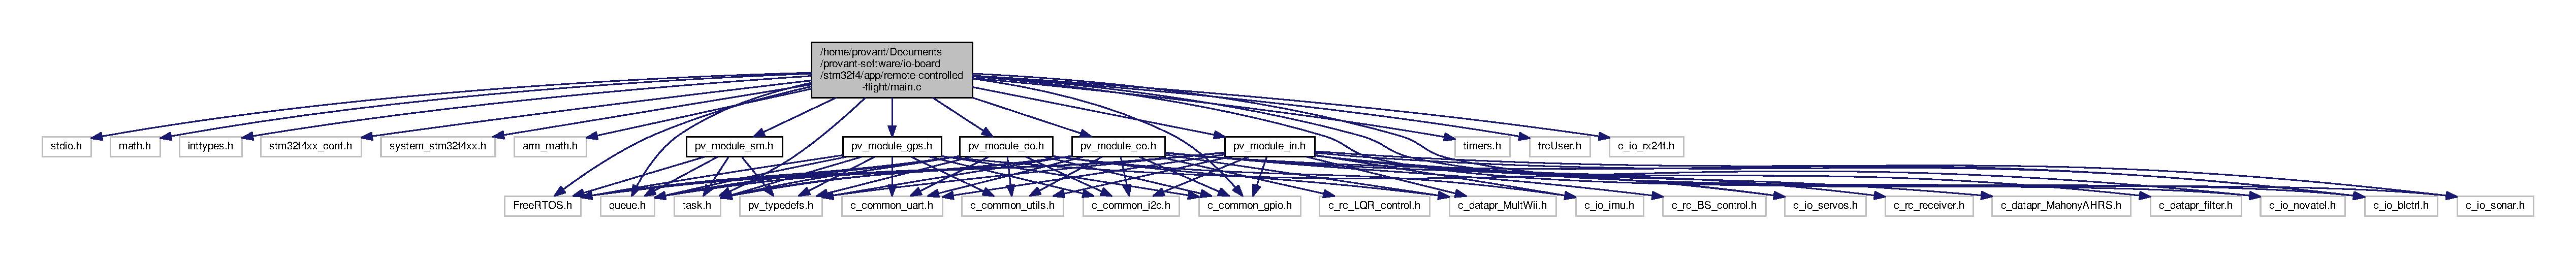
\includegraphics[width=350pt]{main_8c__incl}
\end{center}
\end{figure}
\subsection*{Macros}
\begin{DoxyCompactItemize}
\item 
\#define \hyperlink{main_8c_a42e162ee7b8b8c2663d1dbd31c7b590b}{A\+R\+M\+\_\+\+M\+A\+T\+H\+\_\+\+C\+M4}
\end{DoxyCompactItemize}
\subsection*{Functions}
\begin{DoxyCompactItemize}
\item 
void \hyperlink{group__ProVANT__Modules_ga2850b09d1bb227364b5ff6de6f85f740}{v\+Application\+Tick\+Hook} ()
\item 
void \hyperlink{group__ProVANT__Modules_ga11cbdd335da884dec1204e230554bfd9}{v\+Application\+Idle\+Hook} ()
\item 
void \hyperlink{group__ProVANT__Modules_ga8f5b98d87cfd1379b8d6573159bcbdd3}{v\+Application\+Stack\+Overflow\+Hook} ()
\item 
void \hyperlink{group__ProVANT__Modules_ga73f6aa45470ada02a5d6f3a522d8f13c}{v\+Application\+Malloc\+Failed\+Hook} ()
\item 
void \hyperlink{group__ProVANT__Modules_ga73e2a1fcfc7e7f2bb22937e543997019}{F\+P\+U\+\_\+init} ()
\item 
void \hyperlink{group__ProVANT__Modules_ga39e7a5088757fe328c0162fe25d907bf}{blink\+\_\+led\+\_\+task} (void $\ast$pv\+Parameters)
\item 
void \hyperlink{group__ProVANT__Modules_gab0c5d271dba436247302632e599731ba}{module\+\_\+co\+\_\+task} (void $\ast$pv\+Parameters)
\item 
void \hyperlink{group__ProVANT__Modules_ga7de15cbee9a0ca9eafb3eb25f5e3d691}{module\+\_\+in\+\_\+task} (void $\ast$pv\+Parameters)
\item 
void \hyperlink{group__ProVANT__Modules_ga466679da7a6953ce332271681ce397c7}{module\+\_\+do\+\_\+task} (void $\ast$pv\+Parameters)
\item 
void \hyperlink{group__ProVANT__Modules_gac55e5b60dffafe957dddc7aa452bfa9d}{module\+\_\+gps\+\_\+task} (void $\ast$pv\+Parameters)
\item 
void \hyperlink{group__ProVANT__Modules_gaad8bcaa035ca56eddd3ccbf522298711}{module\+\_\+sm\+\_\+task} (void $\ast$pv\+Parameters)
\item 
int \hyperlink{group__ProVANT__Modules_ga840291bc02cba5474a4cb46a9b9566fe}{main} (void)
\end{DoxyCompactItemize}


\subsection{Detailed Description}
Startup do projeto. 

\begin{DoxyAuthor}{Author}
Martin Vincent Bloedorn \& Patrick José Pereira 
\end{DoxyAuthor}
\begin{DoxyVersion}{Version}
V1.\+0.\+0 
\end{DoxyVersion}
\begin{DoxyDate}{Date}
27-\/\+August-\/2014 
\end{DoxyDate}
\begin{DoxyWarning}{Warning}
Modificar os arquivos provant-\/software/io-\/board/stm32f4/common/modules/common/stm32f4xx\+\_\+conf.\+h provant-\/software/io-\/board/stm32f4/lib/cmsis/inc/stm32f4xx.\+h provant-\/software/io-\/board/stm32f4/lib/cmsis/inc/stm32f4xx\+\_\+conf.\+h dependendo da placa que esta trabalhando. Recompilando com\+: make allclean make T\+O\+DO 
\end{DoxyWarning}


\subsection{Macro Definition Documentation}
\index{main.\+c@{main.\+c}!A\+R\+M\+\_\+\+M\+A\+T\+H\+\_\+\+C\+M4@{A\+R\+M\+\_\+\+M\+A\+T\+H\+\_\+\+C\+M4}}
\index{A\+R\+M\+\_\+\+M\+A\+T\+H\+\_\+\+C\+M4@{A\+R\+M\+\_\+\+M\+A\+T\+H\+\_\+\+C\+M4}!main.\+c@{main.\+c}}
\subsubsection[{\texorpdfstring{A\+R\+M\+\_\+\+M\+A\+T\+H\+\_\+\+C\+M4}{ARM_MATH_CM4}}]{\setlength{\rightskip}{0pt plus 5cm}\#define A\+R\+M\+\_\+\+M\+A\+T\+H\+\_\+\+C\+M4}\hypertarget{main_8c_a42e162ee7b8b8c2663d1dbd31c7b590b}{}\label{main_8c_a42e162ee7b8b8c2663d1dbd31c7b590b}


Definition at line 29 of file main.\+c.


\hypertarget{pv__module__co_8c}{}\section{/home/provant/\+Documents/provant-\/software/io-\/board/stm32f4/app/remote-\/controlled-\/flight/pv\+\_\+module\+\_\+co.c File Reference}
\label{pv__module__co_8c}\index{/home/provant/\+Documents/provant-\/software/io-\/board/stm32f4/app/remote-\/controlled-\/flight/pv\+\_\+module\+\_\+co.\+c@{/home/provant/\+Documents/provant-\/software/io-\/board/stm32f4/app/remote-\/controlled-\/flight/pv\+\_\+module\+\_\+co.\+c}}
{\ttfamily \#include \char`\"{}pv\+\_\+module\+\_\+co.\+h\char`\"{}}\\*
Include dependency graph for pv\+\_\+module\+\_\+co.\+c\+:\nopagebreak
\begin{figure}[H]
\begin{center}
\leavevmode
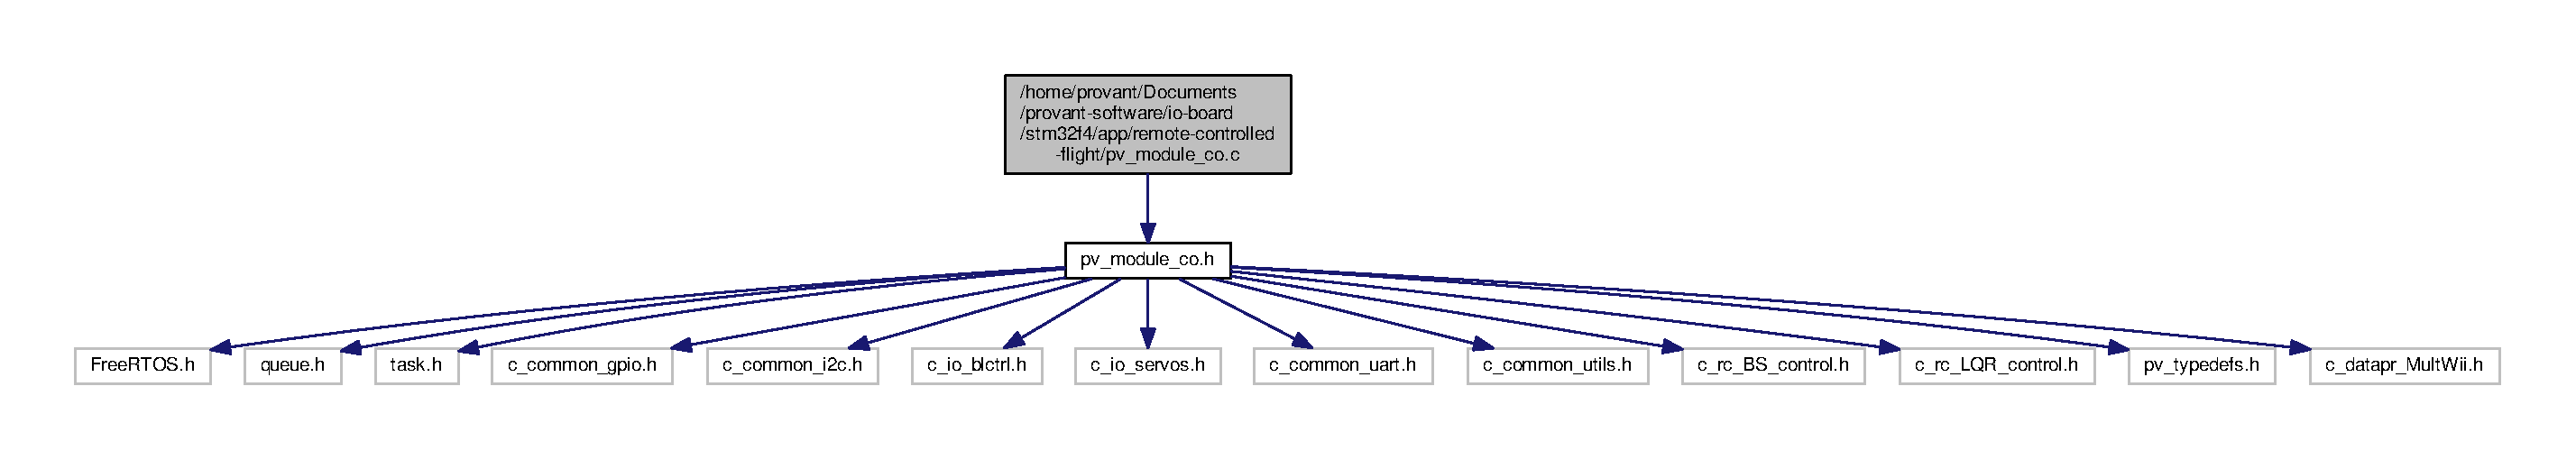
\includegraphics[width=350pt]{pv__module__co_8c__incl}
\end{center}
\end{figure}
\subsection*{Macros}
\begin{DoxyCompactItemize}
\item 
\#define \hyperlink{group__app__co_ga0ac6c9f2991b096e49c354e5cce6fae0}{M\+O\+D\+U\+L\+E\+\_\+\+P\+E\+R\+I\+OD}~12
\item 
\#define \hyperlink{group__app__co_gaec8246e954743c1eca3ed9d0b934bf8e}{E\+S\+C\+\_\+\+ON}~1
\item 
\#define \hyperlink{group__app__co_ga162e9e4abd94f1558733bbf17fca28e9}{S\+E\+R\+V\+O\+\_\+\+ON}~1
\item 
\#define \hyperlink{group__app__co_ga6a53a6c94a70cc286e300a0ea8f46ba4}{U\+S\+A\+R\+T\+\_\+\+B\+A\+U\+D\+R\+A\+TE}~921600
\end{DoxyCompactItemize}
\subsection*{Functions}
\begin{DoxyCompactItemize}
\item 
unsigned char \hyperlink{group__app__co_gac9b9b4433da08cf375a9089fbb464b74}{set\+Point\+E\+S\+C\+\_\+\+Forca} (float forca)
\item 
void \hyperlink{group__app__co_gabedb9a5c3739466a359c93b3585a3640}{module\+\_\+co\+\_\+init} ()
\begin{DoxyCompactList}\small\item\em Inicializacao do módulo de controle + output. \end{DoxyCompactList}\item 
void \hyperlink{group__app__co_gaab8216fc955d01b47e3431aae288d9d3}{module\+\_\+co\+\_\+run} ()
\begin{DoxyCompactList}\small\item\em Função principal do módulo de RC. \end{DoxyCompactList}\end{DoxyCompactItemize}
\subsection*{Variables}
\begin{DoxyCompactItemize}
\item 
port\+Tick\+Type \hyperlink{group__app__co_gab06dc9c7b584f053bcde9e3dd366c886}{pv\+\_\+module\+\_\+co\+\_\+last\+Wake\+Time}
\item 
pv\+\_\+msg\+\_\+input \hyperlink{group__app__co_gac40b8cfe5fd2000670ad57fe3e75ec89}{i\+Input\+Data}
\item 
pv\+\_\+msg\+\_\+control\+Output \hyperlink{group__app__co_ga01528088e36182dce9f2d7126db89886}{i\+Control\+Beagle\+Data}
\item 
pv\+\_\+msg\+\_\+control\+Output \hyperlink{group__app__co_ga0a14ca4568444d2d76c256fa91585cdf}{o\+Control\+Output\+Data}
\item 
pv\+\_\+type\+\_\+actuation \hyperlink{group__app__co_gaf0fb0cf3bcfc492356d3cbe85376efa3}{pv\+\_\+module\+\_\+co\+\_\+actuation}
\item 
int \hyperlink{group__app__co_ga4e39239e9a359dfd174056754a046b8a}{pv\+\_\+module\+\_\+co\+\_\+flag}
\item 
G\+P\+I\+O\+Pin \hyperlink{group__app__co_gaa7d4da6aed3ca0087db45a3706ef17fa}{pv\+\_\+module\+\_\+co\+\_\+\+L\+E\+D5}
\item 
pv\+\_\+type\+\_\+actuation \hyperlink{group__app__co_gaf6cc28f22186e2338a688b8e76d8c975}{i\+Actuation}
\end{DoxyCompactItemize}

\hypertarget{pv__module__co_8h}{}\section{/home/provant/\+Documents/provant-\/software/io-\/board/stm32f4/app/remote-\/controlled-\/flight/pv\+\_\+module\+\_\+co.h File Reference}
\label{pv__module__co_8h}\index{/home/provant/\+Documents/provant-\/software/io-\/board/stm32f4/app/remote-\/controlled-\/flight/pv\+\_\+module\+\_\+co.\+h@{/home/provant/\+Documents/provant-\/software/io-\/board/stm32f4/app/remote-\/controlled-\/flight/pv\+\_\+module\+\_\+co.\+h}}
{\ttfamily \#include \char`\"{}Free\+R\+T\+O\+S.\+h\char`\"{}}\\*
{\ttfamily \#include \char`\"{}queue.\+h\char`\"{}}\\*
{\ttfamily \#include \char`\"{}task.\+h\char`\"{}}\\*
{\ttfamily \#include \char`\"{}c\+\_\+common\+\_\+gpio.\+h\char`\"{}}\\*
{\ttfamily \#include \char`\"{}c\+\_\+common\+\_\+i2c.\+h\char`\"{}}\\*
{\ttfamily \#include \char`\"{}c\+\_\+io\+\_\+blctrl.\+h\char`\"{}}\\*
{\ttfamily \#include \char`\"{}c\+\_\+io\+\_\+servos.\+h\char`\"{}}\\*
{\ttfamily \#include \char`\"{}c\+\_\+common\+\_\+uart.\+h\char`\"{}}\\*
{\ttfamily \#include \char`\"{}c\+\_\+common\+\_\+utils.\+h\char`\"{}}\\*
{\ttfamily \#include \char`\"{}c\+\_\+rc\+\_\+\+B\+S\+\_\+control.\+h\char`\"{}}\\*
{\ttfamily \#include \char`\"{}c\+\_\+rc\+\_\+\+L\+Q\+R\+\_\+control.\+h\char`\"{}}\\*
{\ttfamily \#include \char`\"{}pv\+\_\+typedefs.\+h\char`\"{}}\\*
{\ttfamily \#include \char`\"{}c\+\_\+datapr\+\_\+\+Mult\+Wii.\+h\char`\"{}}\\*
Include dependency graph for pv\+\_\+module\+\_\+co.\+h\+:\nopagebreak
\begin{figure}[H]
\begin{center}
\leavevmode
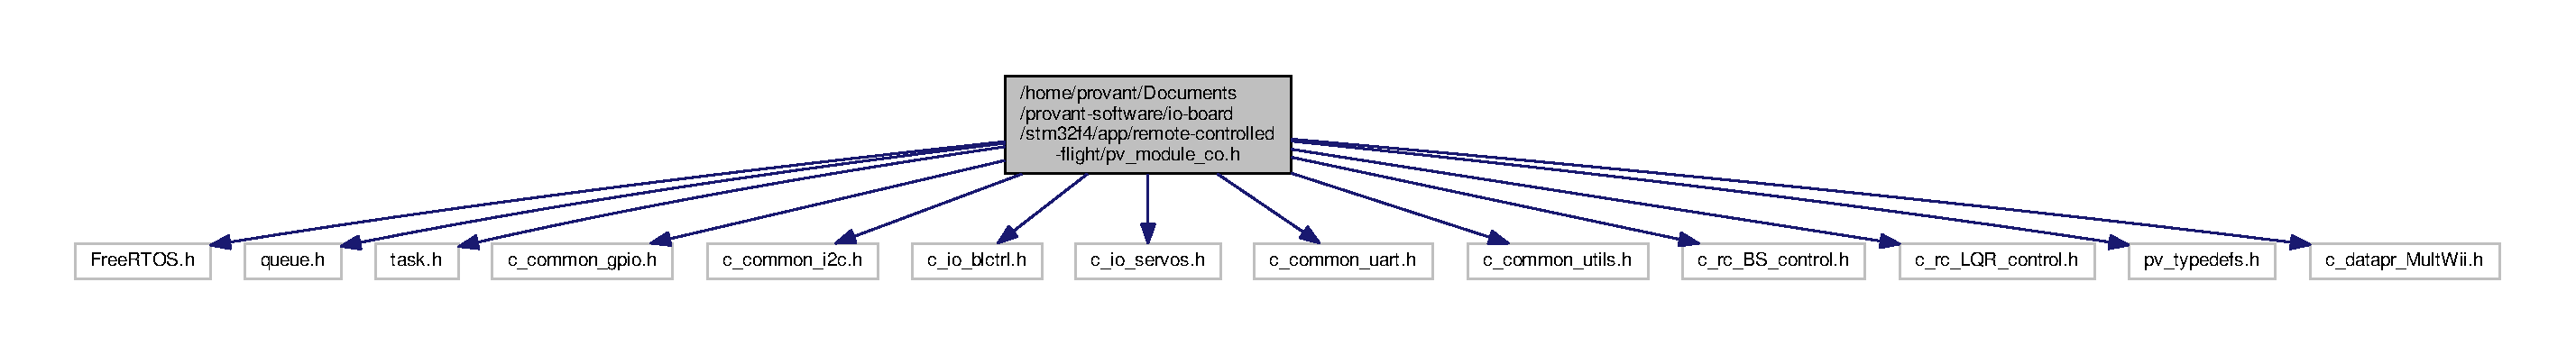
\includegraphics[width=350pt]{pv__module__co_8h__incl}
\end{center}
\end{figure}
This graph shows which files directly or indirectly include this file\+:\nopagebreak
\begin{figure}[H]
\begin{center}
\leavevmode
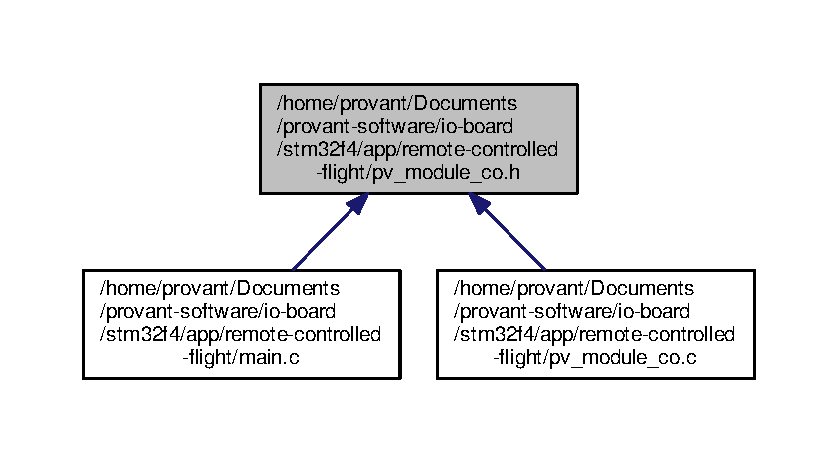
\includegraphics[width=350pt]{pv__module__co_8h__dep__incl}
\end{center}
\end{figure}
\subsection*{Data Structures}
\begin{DoxyCompactItemize}
\item 
struct \hyperlink{structpv__interface__co}{pv\+\_\+interface\+\_\+co}
\end{DoxyCompactItemize}
\subsection*{Macros}
\begin{DoxyCompactItemize}
\item 
\#define \hyperlink{pv__module__co_8h_a09b2b07f1cc6f02982aaa2d3adf4f3ef}{E\+S\+C\+\_\+\+M\+I\+N\+I\+M\+U\+M\+\_\+\+V\+E\+L\+O\+C\+I\+TY}~10
\item 
\#define \hyperlink{pv__module__co_8h_ad825ce45a05b0e80e8d97f8cebd1ee76}{E\+N\+A\+B\+L\+E\+\_\+\+S\+E\+R\+VO}
\item 
\#define \hyperlink{pv__module__co_8h_ade5c6c2cf1e7345fdecaf5e74b3e945b}{A\+X\+I2826}
\item 
\#define \hyperlink{pv__module__co_8h_a2cce57def91019d83715f42bb8927241}{E\+N\+A\+B\+L\+E\+\_\+\+E\+SC}
\end{DoxyCompactItemize}
\subsection*{Functions}
\begin{DoxyCompactItemize}
\item 
void \hyperlink{group__app__co_gabedb9a5c3739466a359c93b3585a3640}{module\+\_\+co\+\_\+init} ()
\begin{DoxyCompactList}\small\item\em Inicializacao do módulo de controle + output. \end{DoxyCompactList}\item 
void \hyperlink{group__app__co_gaab8216fc955d01b47e3431aae288d9d3}{module\+\_\+co\+\_\+run} ()
\begin{DoxyCompactList}\small\item\em Função principal do módulo de RC. \end{DoxyCompactList}\end{DoxyCompactItemize}
\subsection*{Variables}
\begin{DoxyCompactItemize}
\item 
struct \hyperlink{structpv__interface__co}{pv\+\_\+interface\+\_\+co} \hyperlink{pv__module__co_8h_a452c8dc095e980ad1742c4c282fa4297}{pv\+\_\+interface\+\_\+co}
\end{DoxyCompactItemize}


\subsection{Macro Definition Documentation}
\index{pv\+\_\+module\+\_\+co.\+h@{pv\+\_\+module\+\_\+co.\+h}!A\+X\+I2826@{A\+X\+I2826}}
\index{A\+X\+I2826@{A\+X\+I2826}!pv\+\_\+module\+\_\+co.\+h@{pv\+\_\+module\+\_\+co.\+h}}
\subsubsection[{\texorpdfstring{A\+X\+I2826}{AXI2826}}]{\setlength{\rightskip}{0pt plus 5cm}\#define A\+X\+I2826}\hypertarget{pv__module__co_8h_ade5c6c2cf1e7345fdecaf5e74b3e945b}{}\label{pv__module__co_8h_ade5c6c2cf1e7345fdecaf5e74b3e945b}


Definition at line 52 of file pv\+\_\+module\+\_\+co.\+h.

\index{pv\+\_\+module\+\_\+co.\+h@{pv\+\_\+module\+\_\+co.\+h}!E\+N\+A\+B\+L\+E\+\_\+\+E\+SC@{E\+N\+A\+B\+L\+E\+\_\+\+E\+SC}}
\index{E\+N\+A\+B\+L\+E\+\_\+\+E\+SC@{E\+N\+A\+B\+L\+E\+\_\+\+E\+SC}!pv\+\_\+module\+\_\+co.\+h@{pv\+\_\+module\+\_\+co.\+h}}
\subsubsection[{\texorpdfstring{E\+N\+A\+B\+L\+E\+\_\+\+E\+SC}{ENABLE_ESC}}]{\setlength{\rightskip}{0pt plus 5cm}\#define E\+N\+A\+B\+L\+E\+\_\+\+E\+SC}\hypertarget{pv__module__co_8h_a2cce57def91019d83715f42bb8927241}{}\label{pv__module__co_8h_a2cce57def91019d83715f42bb8927241}


Definition at line 54 of file pv\+\_\+module\+\_\+co.\+h.

\index{pv\+\_\+module\+\_\+co.\+h@{pv\+\_\+module\+\_\+co.\+h}!E\+N\+A\+B\+L\+E\+\_\+\+S\+E\+R\+VO@{E\+N\+A\+B\+L\+E\+\_\+\+S\+E\+R\+VO}}
\index{E\+N\+A\+B\+L\+E\+\_\+\+S\+E\+R\+VO@{E\+N\+A\+B\+L\+E\+\_\+\+S\+E\+R\+VO}!pv\+\_\+module\+\_\+co.\+h@{pv\+\_\+module\+\_\+co.\+h}}
\subsubsection[{\texorpdfstring{E\+N\+A\+B\+L\+E\+\_\+\+S\+E\+R\+VO}{ENABLE_SERVO}}]{\setlength{\rightskip}{0pt plus 5cm}\#define E\+N\+A\+B\+L\+E\+\_\+\+S\+E\+R\+VO}\hypertarget{pv__module__co_8h_ad825ce45a05b0e80e8d97f8cebd1ee76}{}\label{pv__module__co_8h_ad825ce45a05b0e80e8d97f8cebd1ee76}


Definition at line 51 of file pv\+\_\+module\+\_\+co.\+h.

\index{pv\+\_\+module\+\_\+co.\+h@{pv\+\_\+module\+\_\+co.\+h}!E\+S\+C\+\_\+\+M\+I\+N\+I\+M\+U\+M\+\_\+\+V\+E\+L\+O\+C\+I\+TY@{E\+S\+C\+\_\+\+M\+I\+N\+I\+M\+U\+M\+\_\+\+V\+E\+L\+O\+C\+I\+TY}}
\index{E\+S\+C\+\_\+\+M\+I\+N\+I\+M\+U\+M\+\_\+\+V\+E\+L\+O\+C\+I\+TY@{E\+S\+C\+\_\+\+M\+I\+N\+I\+M\+U\+M\+\_\+\+V\+E\+L\+O\+C\+I\+TY}!pv\+\_\+module\+\_\+co.\+h@{pv\+\_\+module\+\_\+co.\+h}}
\subsubsection[{\texorpdfstring{E\+S\+C\+\_\+\+M\+I\+N\+I\+M\+U\+M\+\_\+\+V\+E\+L\+O\+C\+I\+TY}{ESC_MINIMUM_VELOCITY}}]{\setlength{\rightskip}{0pt plus 5cm}\#define E\+S\+C\+\_\+\+M\+I\+N\+I\+M\+U\+M\+\_\+\+V\+E\+L\+O\+C\+I\+TY~10}\hypertarget{pv__module__co_8h_a09b2b07f1cc6f02982aaa2d3adf4f3ef}{}\label{pv__module__co_8h_a09b2b07f1cc6f02982aaa2d3adf4f3ef}


Definition at line 50 of file pv\+\_\+module\+\_\+co.\+h.



\subsection{Variable Documentation}
\index{pv\+\_\+module\+\_\+co.\+h@{pv\+\_\+module\+\_\+co.\+h}!pv\+\_\+interface\+\_\+co@{pv\+\_\+interface\+\_\+co}}
\index{pv\+\_\+interface\+\_\+co@{pv\+\_\+interface\+\_\+co}!pv\+\_\+module\+\_\+co.\+h@{pv\+\_\+module\+\_\+co.\+h}}
\subsubsection[{\texorpdfstring{pv\+\_\+interface\+\_\+co}{pv_interface_co}}]{\setlength{\rightskip}{0pt plus 5cm}struct {\bf pv\+\_\+interface\+\_\+co}  {\bf pv\+\_\+interface\+\_\+co}}\hypertarget{pv__module__co_8h_a452c8dc095e980ad1742c4c282fa4297}{}\label{pv__module__co_8h_a452c8dc095e980ad1742c4c282fa4297}

\hypertarget{pv__module__do_8c}{}\section{/home/provant/\+Documents/provant-\/software/io-\/board/stm32f4/app/remote-\/controlled-\/flight/pv\+\_\+module\+\_\+do.c File Reference}
\label{pv__module__do_8c}\index{/home/provant/\+Documents/provant-\/software/io-\/board/stm32f4/app/remote-\/controlled-\/flight/pv\+\_\+module\+\_\+do.\+c@{/home/provant/\+Documents/provant-\/software/io-\/board/stm32f4/app/remote-\/controlled-\/flight/pv\+\_\+module\+\_\+do.\+c}}


Implementação do módulo de transmissao de dados para fora do A\+RM.  


{\ttfamily \#include \char`\"{}pv\+\_\+module\+\_\+do.\+h\char`\"{}}\\*
Include dependency graph for pv\+\_\+module\+\_\+do.\+c\+:\nopagebreak
\begin{figure}[H]
\begin{center}
\leavevmode
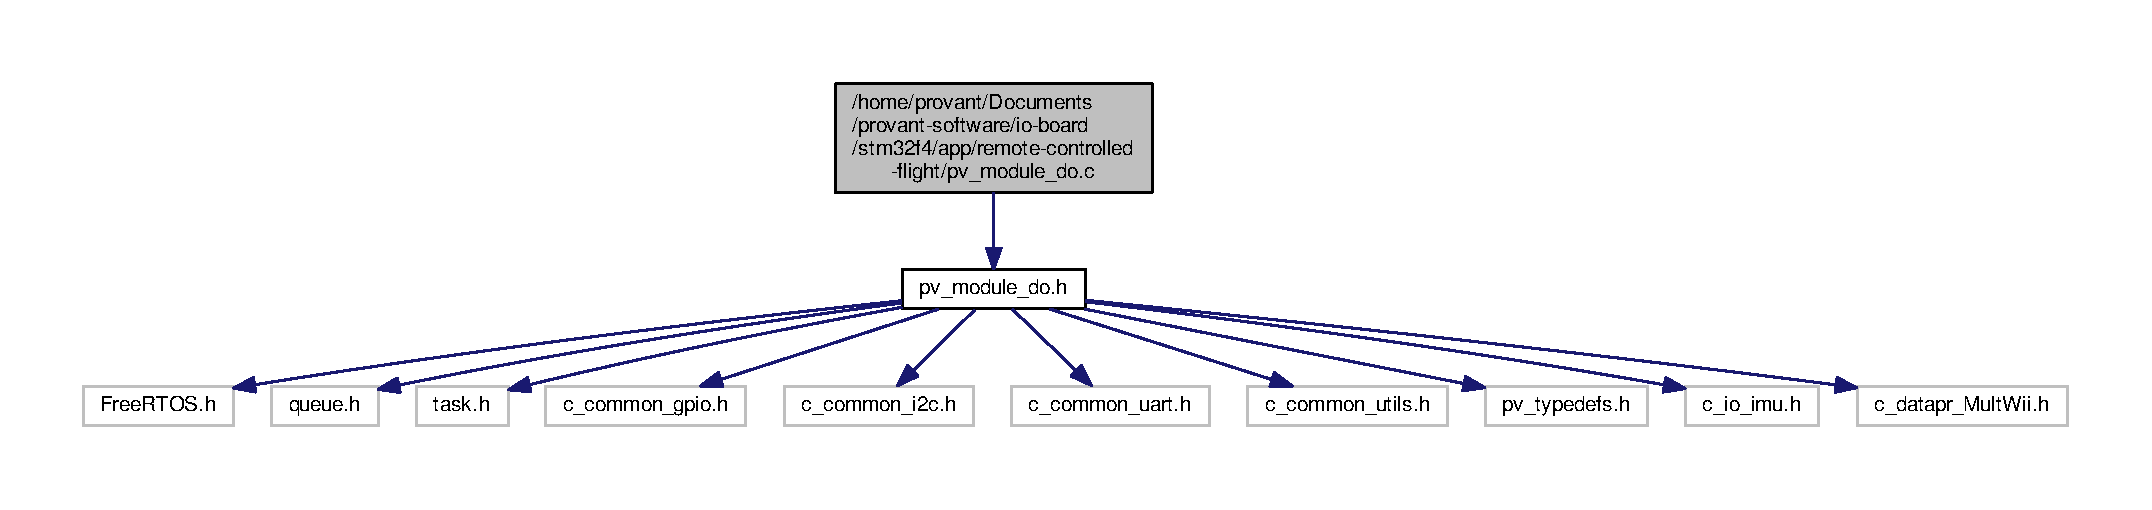
\includegraphics[width=350pt]{pv__module__do_8c__incl}
\end{center}
\end{figure}
\subsection*{Macros}
\begin{DoxyCompactItemize}
\item 
\#define \hyperlink{group__app__do_ga0ac6c9f2991b096e49c354e5cce6fae0}{M\+O\+D\+U\+L\+E\+\_\+\+P\+E\+R\+I\+OD}~15
\item 
\#define \hyperlink{group__app__do_ga6a53a6c94a70cc286e300a0ea8f46ba4}{U\+S\+A\+R\+T\+\_\+\+B\+A\+U\+D\+R\+A\+TE}~921600
\end{DoxyCompactItemize}
\subsection*{Functions}
\begin{DoxyCompactItemize}
\item 
void \hyperlink{group__app__do_ga901c023651503207f5cfd8cdb8c305b3}{module\+\_\+do\+\_\+init} ()
\begin{DoxyCompactList}\small\item\em Inicializacao do módulo de data out. \end{DoxyCompactList}\item 
void \hyperlink{group__app__do_ga1f08b4b431624465a47f47eca0520253}{module\+\_\+do\+\_\+run} ()
\begin{DoxyCompactList}\small\item\em Função principal do módulo de data out. \end{DoxyCompactList}\end{DoxyCompactItemize}
\subsection*{Variables}
\begin{DoxyCompactItemize}
\item 
port\+Tick\+Type \hyperlink{group__app__do_gaa8db3871cb5f64abbd94ddd5a1db73a6}{last\+Wake\+Time}
\item 
unsigned int \hyperlink{group__app__do_ga24475be702ffcc5a6f0a5557040368ef}{heart\+Beat} =0
\item 
unsigned int \hyperlink{group__app__do_ga5bdb7b29978109a480db66886e58f475}{cicle\+Time} =0
\item 
pv\+\_\+msg\+\_\+input \hyperlink{group__app__do_gac40b8cfe5fd2000670ad57fe3e75ec89}{i\+Input\+Data}
\item 
pv\+\_\+msg\+\_\+gps \hyperlink{group__app__do_gac433f205128f94bd944f8ddcbff92744}{i\+Gps\+Data}
\item 
pv\+\_\+msg\+\_\+control\+Output \hyperlink{group__app__do_gacabca53fbaffdbf13b8e5a1c29b73bc4}{i\+Control\+Output\+Data}
\item 
pv\+\_\+msg\+\_\+control\+Output \hyperlink{group__app__do_ga83a7ee8a519c421eec8b1c7efc9e0501}{o\+Control\+Beagle\+Data}
\item 
float \hyperlink{group__app__do_ga1ba0a7c98794a4cda502c52d222ab614}{rpy} \mbox{[}3\mbox{]}
\item 
float \hyperlink{group__app__do_ga09c67ab670708cf621c9853aeb34fc2c}{drpy} \mbox{[}3\mbox{]}
\item 
float \hyperlink{group__app__do_ga1a3ca0a0bf0cdb13a8689c0558ead4df}{position} \mbox{[}3\mbox{]}
\item 
float \hyperlink{group__app__do_ga63a3bb0717d926f2f94b982b96e92237}{velocity} \mbox{[}3\mbox{]}
\item 
float \hyperlink{group__app__do_gaf2c21f3aed6186d912908dcd33a057d6}{alpha} \mbox{[}2\mbox{]}
\item 
float \hyperlink{group__app__do_gac55455b51b6abc065db2bfa3a99c0783}{dalpha} \mbox{[}2\mbox{]}
\item 
float \hyperlink{group__app__do_ga44b306459efc6e5e3543390e98fa8df7}{data1} \mbox{[}2\mbox{]}
\item 
float \hyperlink{group__app__do_ga2241fa8ef7e6a940cd8ce8dc13d8b4e8}{data2} \mbox{[}2\mbox{]}
\item 
float \hyperlink{group__app__do_gafb91c0f3a7dabe2beb8c046ff3cd4613}{data3} \mbox{[}2\mbox{]}
\item 
int \hyperlink{group__app__do_ga5acd447dc75f4ac13cdac246a2c75291}{aux} \mbox{[}2\mbox{]}
\item 
float \hyperlink{group__app__do_gae93eafaee31c92a65f90bcb26eda96df}{aux2} \mbox{[}3\mbox{]}
\item 
float \hyperlink{group__app__do_gaa56fed06b51b312e13aa20c0c740795e}{servo\+Torque} \mbox{[}2\mbox{]}
\item 
float \hyperlink{group__app__do_ga7b919fc59fbb86e34627c65320446dd3}{esc\+Force} \mbox{[}2\mbox{]}
\item 
int \hyperlink{group__app__do_ga7738565d91833be3229136a1beaaf44b}{channel} \mbox{[}7\mbox{]}
\item 
G\+P\+I\+O\+Pin \hyperlink{group__app__do_ga804d3aba22a782022afc3977966f2faa}{L\+E\+D3}
\end{DoxyCompactItemize}


\subsection{Detailed Description}
Implementação do módulo de transmissao de dados para fora do A\+RM. 

\begin{DoxyAuthor}{Author}
Patrick Jose Pereira 
\end{DoxyAuthor}
\begin{DoxyVersion}{Version}
V1.\+0.\+0 
\end{DoxyVersion}
\begin{DoxyDate}{Date}
27-\/\+August-\/2014 
\end{DoxyDate}

\hypertarget{pv__module__do_8h}{}\section{/home/provant/\+Documents/provant-\/software/io-\/board/stm32f4/app/remote-\/controlled-\/flight/pv\+\_\+module\+\_\+do.h File Reference}
\label{pv__module__do_8h}\index{/home/provant/\+Documents/provant-\/software/io-\/board/stm32f4/app/remote-\/controlled-\/flight/pv\+\_\+module\+\_\+do.\+h@{/home/provant/\+Documents/provant-\/software/io-\/board/stm32f4/app/remote-\/controlled-\/flight/pv\+\_\+module\+\_\+do.\+h}}


Implementação do módulo de transmissao de dados para fora do A\+RM.  


{\ttfamily \#include \char`\"{}Free\+R\+T\+O\+S.\+h\char`\"{}}\\*
{\ttfamily \#include \char`\"{}queue.\+h\char`\"{}}\\*
{\ttfamily \#include \char`\"{}task.\+h\char`\"{}}\\*
{\ttfamily \#include \char`\"{}c\+\_\+common\+\_\+gpio.\+h\char`\"{}}\\*
{\ttfamily \#include \char`\"{}c\+\_\+common\+\_\+i2c.\+h\char`\"{}}\\*
{\ttfamily \#include \char`\"{}c\+\_\+common\+\_\+uart.\+h\char`\"{}}\\*
{\ttfamily \#include \char`\"{}c\+\_\+common\+\_\+utils.\+h\char`\"{}}\\*
{\ttfamily \#include \char`\"{}pv\+\_\+typedefs.\+h\char`\"{}}\\*
{\ttfamily \#include \char`\"{}c\+\_\+io\+\_\+imu.\+h\char`\"{}}\\*
{\ttfamily \#include \char`\"{}c\+\_\+datapr\+\_\+\+Mult\+Wii.\+h\char`\"{}}\\*
Include dependency graph for pv\+\_\+module\+\_\+do.\+h\+:\nopagebreak
\begin{figure}[H]
\begin{center}
\leavevmode
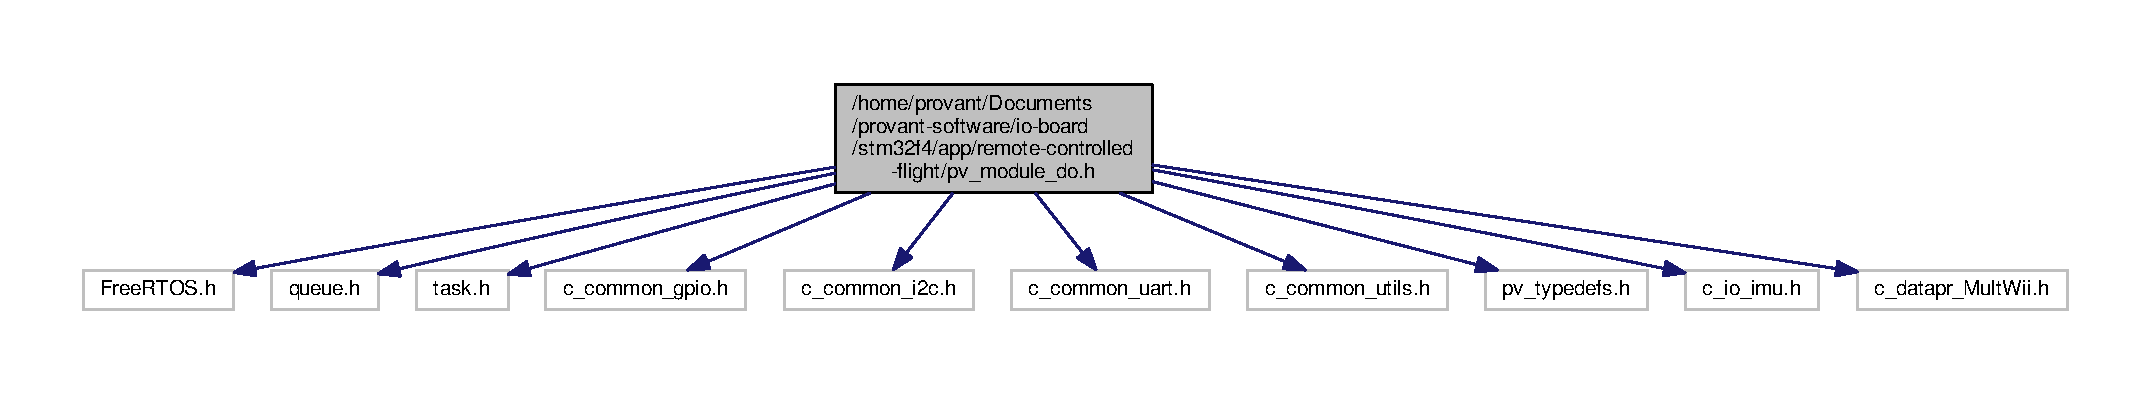
\includegraphics[width=350pt]{pv__module__do_8h__incl}
\end{center}
\end{figure}
This graph shows which files directly or indirectly include this file\+:\nopagebreak
\begin{figure}[H]
\begin{center}
\leavevmode
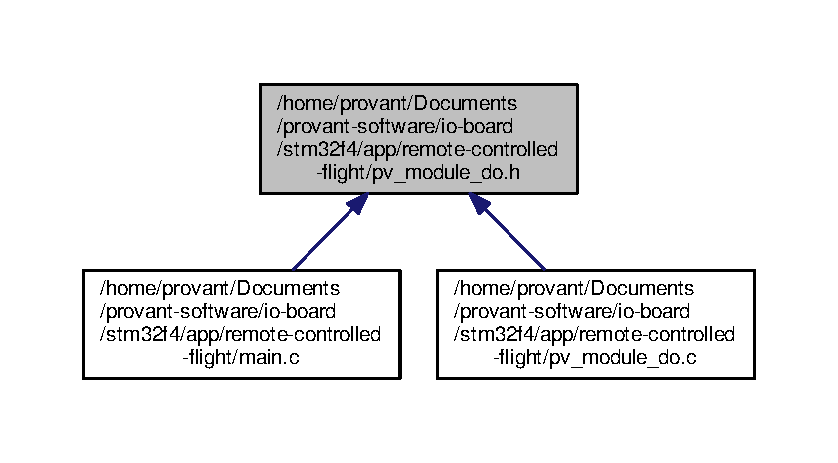
\includegraphics[width=350pt]{pv__module__do_8h__dep__incl}
\end{center}
\end{figure}
\subsection*{Data Structures}
\begin{DoxyCompactItemize}
\item 
struct \hyperlink{structpv__interface__do}{pv\+\_\+interface\+\_\+do}
\end{DoxyCompactItemize}
\subsection*{Functions}
\begin{DoxyCompactItemize}
\item 
void \hyperlink{group__app__do_ga901c023651503207f5cfd8cdb8c305b3}{module\+\_\+do\+\_\+init} ()
\begin{DoxyCompactList}\small\item\em Inicializacao do módulo de data out. \end{DoxyCompactList}\item 
void \hyperlink{group__app__do_ga1f08b4b431624465a47f47eca0520253}{module\+\_\+do\+\_\+run} ()
\begin{DoxyCompactList}\small\item\em Função principal do módulo de data out. \end{DoxyCompactList}\end{DoxyCompactItemize}
\subsection*{Variables}
\begin{DoxyCompactItemize}
\item 
struct \hyperlink{structpv__interface__do}{pv\+\_\+interface\+\_\+do} \hyperlink{pv__module__do_8h_acdcb55c89a8823c672940a0901d30868}{pv\+\_\+interface\+\_\+do}
\end{DoxyCompactItemize}


\subsection{Detailed Description}
Implementação do módulo de transmissao de dados para fora do A\+RM. 

\begin{DoxyAuthor}{Author}
Patrick Jose Pereira 
\end{DoxyAuthor}
\begin{DoxyVersion}{Version}
V1.\+0.\+0 
\end{DoxyVersion}
\begin{DoxyDate}{Date}
27-\/\+August-\/2014 
\end{DoxyDate}


\subsection{Variable Documentation}
\index{pv\+\_\+module\+\_\+do.\+h@{pv\+\_\+module\+\_\+do.\+h}!pv\+\_\+interface\+\_\+do@{pv\+\_\+interface\+\_\+do}}
\index{pv\+\_\+interface\+\_\+do@{pv\+\_\+interface\+\_\+do}!pv\+\_\+module\+\_\+do.\+h@{pv\+\_\+module\+\_\+do.\+h}}
\subsubsection[{\texorpdfstring{pv\+\_\+interface\+\_\+do}{pv_interface_do}}]{\setlength{\rightskip}{0pt plus 5cm}struct {\bf pv\+\_\+interface\+\_\+do}  {\bf pv\+\_\+interface\+\_\+do}}\hypertarget{pv__module__do_8h_acdcb55c89a8823c672940a0901d30868}{}\label{pv__module__do_8h_acdcb55c89a8823c672940a0901d30868}

\hypertarget{pv__module__gps_8c}{}\section{/home/provant/\+Documents/provant-\/software/io-\/board/stm32f4/app/remote-\/controlled-\/flight/pv\+\_\+module\+\_\+gps.c File Reference}
\label{pv__module__gps_8c}\index{/home/provant/\+Documents/provant-\/software/io-\/board/stm32f4/app/remote-\/controlled-\/flight/pv\+\_\+module\+\_\+gps.\+c@{/home/provant/\+Documents/provant-\/software/io-\/board/stm32f4/app/remote-\/controlled-\/flight/pv\+\_\+module\+\_\+gps.\+c}}


Implementação do módulo de leitura de dados do G\+PS.  


{\ttfamily \#include \char`\"{}pv\+\_\+module\+\_\+gps.\+h\char`\"{}}\\*
Include dependency graph for pv\+\_\+module\+\_\+gps.\+c\+:\nopagebreak
\begin{figure}[H]
\begin{center}
\leavevmode
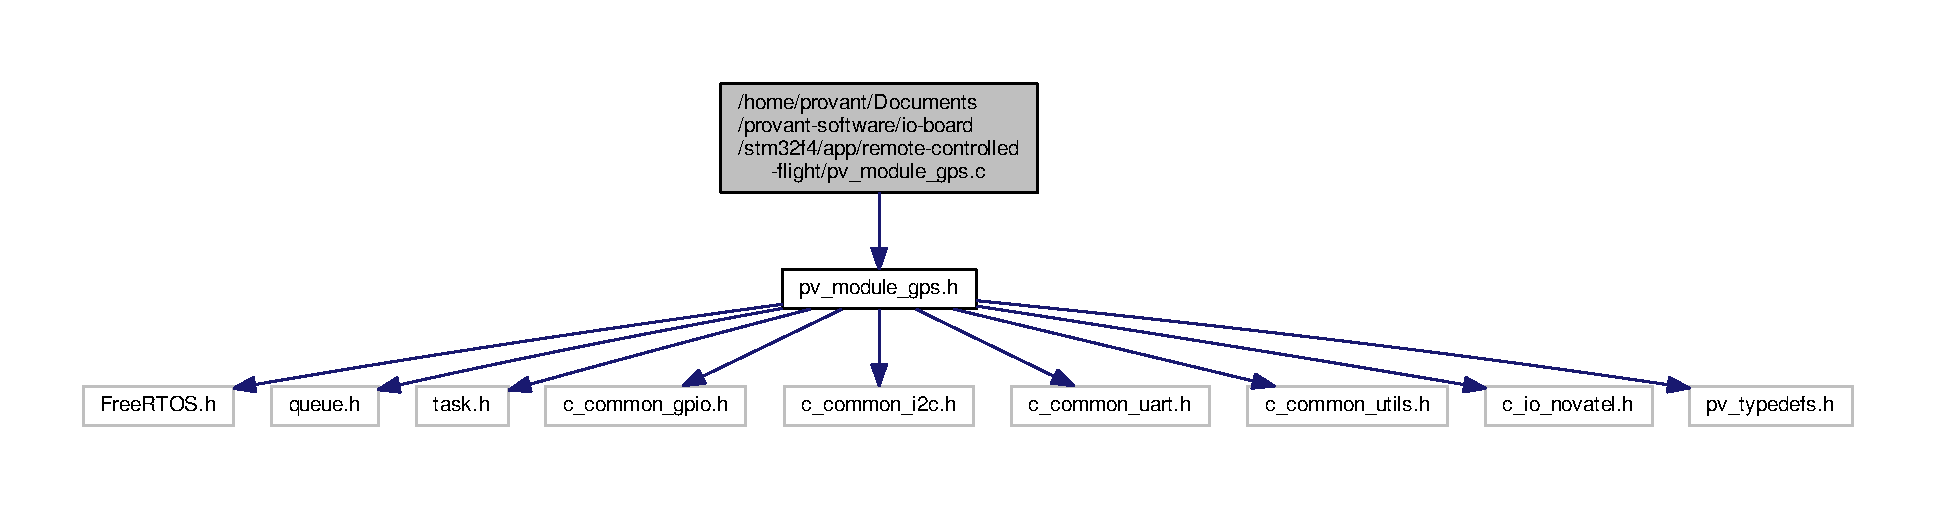
\includegraphics[width=350pt]{pv__module__gps_8c__incl}
\end{center}
\end{figure}
\subsection*{Macros}
\begin{DoxyCompactItemize}
\item 
\#define \hyperlink{group__app__gps_ga0ac6c9f2991b096e49c354e5cce6fae0}{M\+O\+D\+U\+L\+E\+\_\+\+P\+E\+R\+I\+OD}~100
\end{DoxyCompactItemize}
\subsection*{Functions}
\begin{DoxyCompactItemize}
\item 
void \hyperlink{group__app__gps_ga9ee93102a0a5aec6877376bbcaf1dcb0}{module\+\_\+gps\+\_\+init} ()
\begin{DoxyCompactList}\small\item\em Inicializacao do módulo de G\+PS. \end{DoxyCompactList}\item 
void \hyperlink{group__app__gps_gace423457cfae0d22bd57db9e2fb4c033}{module\+\_\+gps\+\_\+run} ()
\begin{DoxyCompactList}\small\item\em Função principal do módulo de G\+PS. \end{DoxyCompactList}\end{DoxyCompactItemize}
\subsection*{Variables}
\begin{DoxyCompactItemize}
\item 
port\+Tick\+Type \hyperlink{group__app__gps_gaa8db3871cb5f64abbd94ddd5a1db73a6}{last\+Wake\+Time}
\item 
pv\+\_\+msg\+\_\+gps \hyperlink{group__app__gps_ga744821cc9c45de009ae70e6dc8d5e220}{o\+Gps\+Data}
\item 
pv\+\_\+msg\+\_\+control\+Output \hyperlink{group__app__gps_ga0a14ca4568444d2d76c256fa91585cdf}{o\+Control\+Output\+Data}
\end{DoxyCompactItemize}


\subsection{Detailed Description}
Implementação do módulo de leitura de dados do G\+PS. 

\begin{DoxyAuthor}{Author}
Patrick Jose Pereira 
\end{DoxyAuthor}
\begin{DoxyVersion}{Version}
V1.\+0.\+0 
\end{DoxyVersion}
\begin{DoxyDate}{Date}
27-\/\+August-\/2014 
\end{DoxyDate}

\hypertarget{pv__module__gps_8h}{}\section{/home/provant/\+Documents/provant-\/software/io-\/board/stm32f4/app/remote-\/controlled-\/flight/pv\+\_\+module\+\_\+gps.h File Reference}
\label{pv__module__gps_8h}\index{/home/provant/\+Documents/provant-\/software/io-\/board/stm32f4/app/remote-\/controlled-\/flight/pv\+\_\+module\+\_\+gps.\+h@{/home/provant/\+Documents/provant-\/software/io-\/board/stm32f4/app/remote-\/controlled-\/flight/pv\+\_\+module\+\_\+gps.\+h}}


Implementação do módulo de leitura de dados do G\+PS.  


{\ttfamily \#include \char`\"{}Free\+R\+T\+O\+S.\+h\char`\"{}}\\*
{\ttfamily \#include \char`\"{}queue.\+h\char`\"{}}\\*
{\ttfamily \#include \char`\"{}task.\+h\char`\"{}}\\*
{\ttfamily \#include \char`\"{}c\+\_\+common\+\_\+gpio.\+h\char`\"{}}\\*
{\ttfamily \#include \char`\"{}c\+\_\+common\+\_\+i2c.\+h\char`\"{}}\\*
{\ttfamily \#include \char`\"{}c\+\_\+common\+\_\+uart.\+h\char`\"{}}\\*
{\ttfamily \#include \char`\"{}c\+\_\+common\+\_\+utils.\+h\char`\"{}}\\*
{\ttfamily \#include \char`\"{}c\+\_\+io\+\_\+novatel.\+h\char`\"{}}\\*
{\ttfamily \#include \char`\"{}pv\+\_\+typedefs.\+h\char`\"{}}\\*
Include dependency graph for pv\+\_\+module\+\_\+gps.\+h\+:\nopagebreak
\begin{figure}[H]
\begin{center}
\leavevmode
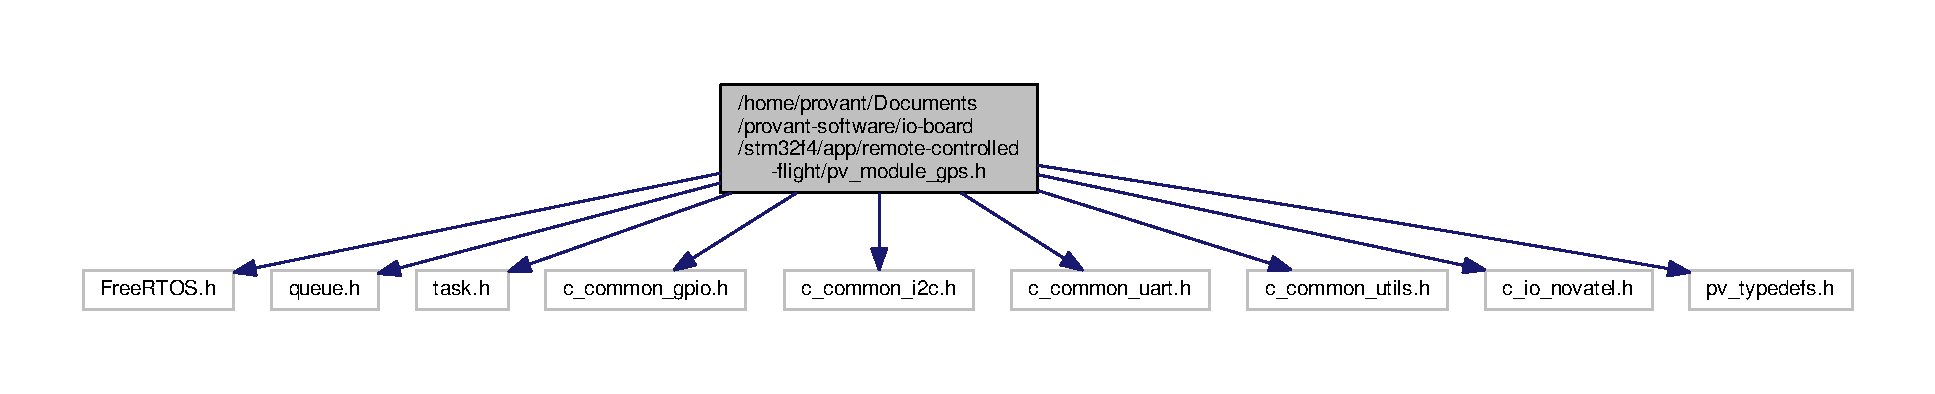
\includegraphics[width=350pt]{pv__module__gps_8h__incl}
\end{center}
\end{figure}
This graph shows which files directly or indirectly include this file\+:\nopagebreak
\begin{figure}[H]
\begin{center}
\leavevmode
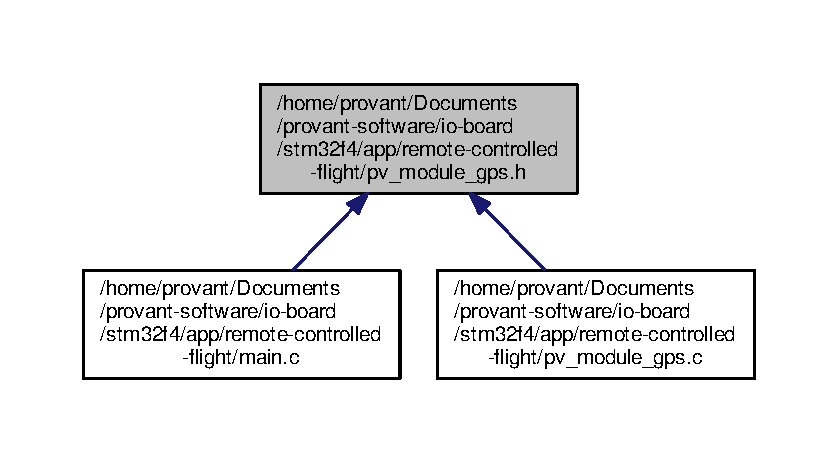
\includegraphics[width=350pt]{pv__module__gps_8h__dep__incl}
\end{center}
\end{figure}
\subsection*{Data Structures}
\begin{DoxyCompactItemize}
\item 
struct \hyperlink{structpv__interface__gps}{pv\+\_\+interface\+\_\+gps}
\end{DoxyCompactItemize}
\subsection*{Functions}
\begin{DoxyCompactItemize}
\item 
void \hyperlink{group__app__gps_ga9ee93102a0a5aec6877376bbcaf1dcb0}{module\+\_\+gps\+\_\+init} ()
\begin{DoxyCompactList}\small\item\em Inicializacao do módulo de G\+PS. \end{DoxyCompactList}\item 
void \hyperlink{group__app__gps_gace423457cfae0d22bd57db9e2fb4c033}{module\+\_\+gps\+\_\+run} ()
\begin{DoxyCompactList}\small\item\em Função principal do módulo de G\+PS. \end{DoxyCompactList}\end{DoxyCompactItemize}
\subsection*{Variables}
\begin{DoxyCompactItemize}
\item 
struct \hyperlink{structpv__interface__gps}{pv\+\_\+interface\+\_\+gps} \hyperlink{pv__module__gps_8h_a775804c5a6320fe3d55e009d0aed6363}{pv\+\_\+interface\+\_\+gps}
\end{DoxyCompactItemize}


\subsection{Detailed Description}
Implementação do módulo de leitura de dados do G\+PS. 

\begin{DoxyAuthor}{Author}
Patrick Jose Pereira 
\end{DoxyAuthor}
\begin{DoxyVersion}{Version}
V1.\+0.\+0 
\end{DoxyVersion}
\begin{DoxyDate}{Date}
27-\/\+August-\/2014 
\end{DoxyDate}


\subsection{Variable Documentation}
\index{pv\+\_\+module\+\_\+gps.\+h@{pv\+\_\+module\+\_\+gps.\+h}!pv\+\_\+interface\+\_\+gps@{pv\+\_\+interface\+\_\+gps}}
\index{pv\+\_\+interface\+\_\+gps@{pv\+\_\+interface\+\_\+gps}!pv\+\_\+module\+\_\+gps.\+h@{pv\+\_\+module\+\_\+gps.\+h}}
\subsubsection[{\texorpdfstring{pv\+\_\+interface\+\_\+gps}{pv_interface_gps}}]{\setlength{\rightskip}{0pt plus 5cm}struct {\bf pv\+\_\+interface\+\_\+gps}  {\bf pv\+\_\+interface\+\_\+gps}}\hypertarget{pv__module__gps_8h_a775804c5a6320fe3d55e009d0aed6363}{}\label{pv__module__gps_8h_a775804c5a6320fe3d55e009d0aed6363}

\hypertarget{pv__module__in_8c}{}\section{/home/provant/\+Documents/provant-\/software/io-\/board/stm32f4/app/remote-\/controlled-\/flight/pv\+\_\+module\+\_\+in.c File Reference}
\label{pv__module__in_8c}\index{/home/provant/\+Documents/provant-\/software/io-\/board/stm32f4/app/remote-\/controlled-\/flight/pv\+\_\+module\+\_\+in.\+c@{/home/provant/\+Documents/provant-\/software/io-\/board/stm32f4/app/remote-\/controlled-\/flight/pv\+\_\+module\+\_\+in.\+c}}
{\ttfamily \#include \char`\"{}pv\+\_\+module\+\_\+in.\+h\char`\"{}}\\*
Include dependency graph for pv\+\_\+module\+\_\+in.\+c\+:\nopagebreak
\begin{figure}[H]
\begin{center}
\leavevmode
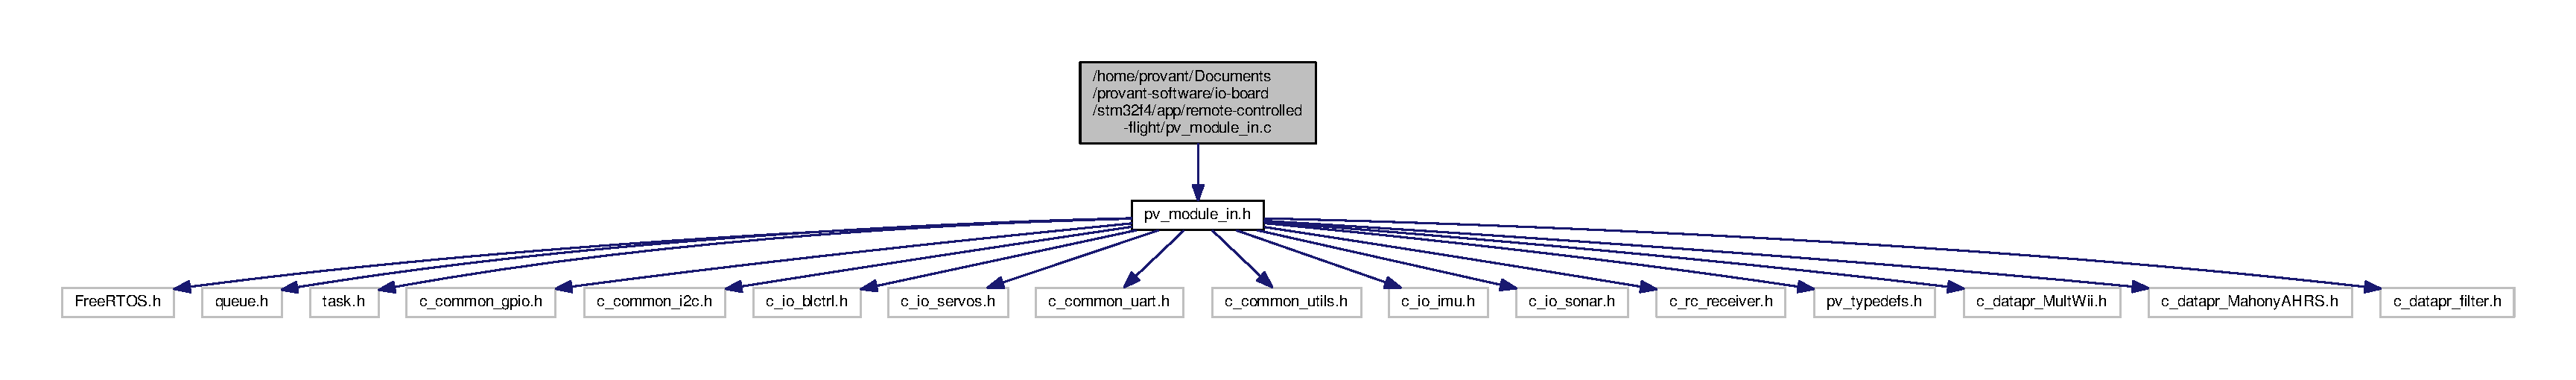
\includegraphics[width=350pt]{pv__module__in_8c__incl}
\end{center}
\end{figure}
\subsection*{Macros}
\begin{DoxyCompactItemize}
\item 
\#define \hyperlink{group__app__in_ga0ac6c9f2991b096e49c354e5cce6fae0}{M\+O\+D\+U\+L\+E\+\_\+\+P\+E\+R\+I\+OD}~6
\end{DoxyCompactItemize}
\subsection*{Functions}
\begin{DoxyCompactItemize}
\item 
void \hyperlink{group__app__in_gaffe0980a750cbec13ebf241c933460dd}{module\+\_\+in\+\_\+init} ()
\begin{DoxyCompactList}\small\item\em Inicializacao componentes de IO. \end{DoxyCompactList}\item 
void \hyperlink{group__app__in_ga2b56089e4c5adb9ac8b7a41fc1a0b0b2}{module\+\_\+in\+\_\+run} ()
\begin{DoxyCompactList}\small\item\em Função principal do módulo de IO. \end{DoxyCompactList}\end{DoxyCompactItemize}
\subsection*{Variables}
\begin{DoxyCompactItemize}
\item 
port\+Tick\+Type \hyperlink{group__app__in_ga3ff9efc032b26284423c9100a5474b7b}{pv\+\_\+module\+\_\+in\+\_\+last\+Wake\+Time}
\item 
char \hyperlink{group__app__in_ga3000f858ecb5a5417c1566b691efd56d}{str} \mbox{[}256\mbox{]}
\item 
G\+P\+I\+O\+Pin \hyperlink{group__app__in_ga8d3f5e0ec53e4667efbebf11383765e4}{pv\+\_\+module\+\_\+in\+\_\+\+L\+E\+D4}
\item 
float \hyperlink{group__app__in_ga926ba5b807f8b3d71b9fb486eb32a508}{attitude\+\_\+quaternion} \mbox{[}4\mbox{]} =\{1,0,0,0\}
\item 
pv\+\_\+msg\+\_\+input \hyperlink{group__app__in_gaffc6f7805bab2d46af160c6f7715ba99}{o\+Input\+Data}
\end{DoxyCompactItemize}

\hypertarget{pv__module__in_8h}{}\section{/home/provant/\+Documents/provant-\/software/io-\/board/stm32f4/app/remote-\/controlled-\/flight/pv\+\_\+module\+\_\+in.h File Reference}
\label{pv__module__in_8h}\index{/home/provant/\+Documents/provant-\/software/io-\/board/stm32f4/app/remote-\/controlled-\/flight/pv\+\_\+module\+\_\+in.\+h@{/home/provant/\+Documents/provant-\/software/io-\/board/stm32f4/app/remote-\/controlled-\/flight/pv\+\_\+module\+\_\+in.\+h}}
{\ttfamily \#include \char`\"{}Free\+R\+T\+O\+S.\+h\char`\"{}}\\*
{\ttfamily \#include \char`\"{}queue.\+h\char`\"{}}\\*
{\ttfamily \#include \char`\"{}task.\+h\char`\"{}}\\*
{\ttfamily \#include \char`\"{}c\+\_\+common\+\_\+gpio.\+h\char`\"{}}\\*
{\ttfamily \#include \char`\"{}c\+\_\+common\+\_\+i2c.\+h\char`\"{}}\\*
{\ttfamily \#include \char`\"{}c\+\_\+io\+\_\+blctrl.\+h\char`\"{}}\\*
{\ttfamily \#include \char`\"{}c\+\_\+io\+\_\+servos.\+h\char`\"{}}\\*
{\ttfamily \#include \char`\"{}c\+\_\+common\+\_\+uart.\+h\char`\"{}}\\*
{\ttfamily \#include \char`\"{}c\+\_\+common\+\_\+utils.\+h\char`\"{}}\\*
{\ttfamily \#include \char`\"{}c\+\_\+io\+\_\+imu.\+h\char`\"{}}\\*
{\ttfamily \#include \char`\"{}c\+\_\+io\+\_\+sonar.\+h\char`\"{}}\\*
{\ttfamily \#include \char`\"{}c\+\_\+rc\+\_\+receiver.\+h\char`\"{}}\\*
{\ttfamily \#include \char`\"{}pv\+\_\+typedefs.\+h\char`\"{}}\\*
{\ttfamily \#include \char`\"{}c\+\_\+datapr\+\_\+\+Mult\+Wii.\+h\char`\"{}}\\*
{\ttfamily \#include \char`\"{}c\+\_\+datapr\+\_\+\+Mahony\+A\+H\+R\+S.\+h\char`\"{}}\\*
{\ttfamily \#include \char`\"{}c\+\_\+datapr\+\_\+filter.\+h\char`\"{}}\\*
Include dependency graph for pv\+\_\+module\+\_\+in.\+h\+:\nopagebreak
\begin{figure}[H]
\begin{center}
\leavevmode
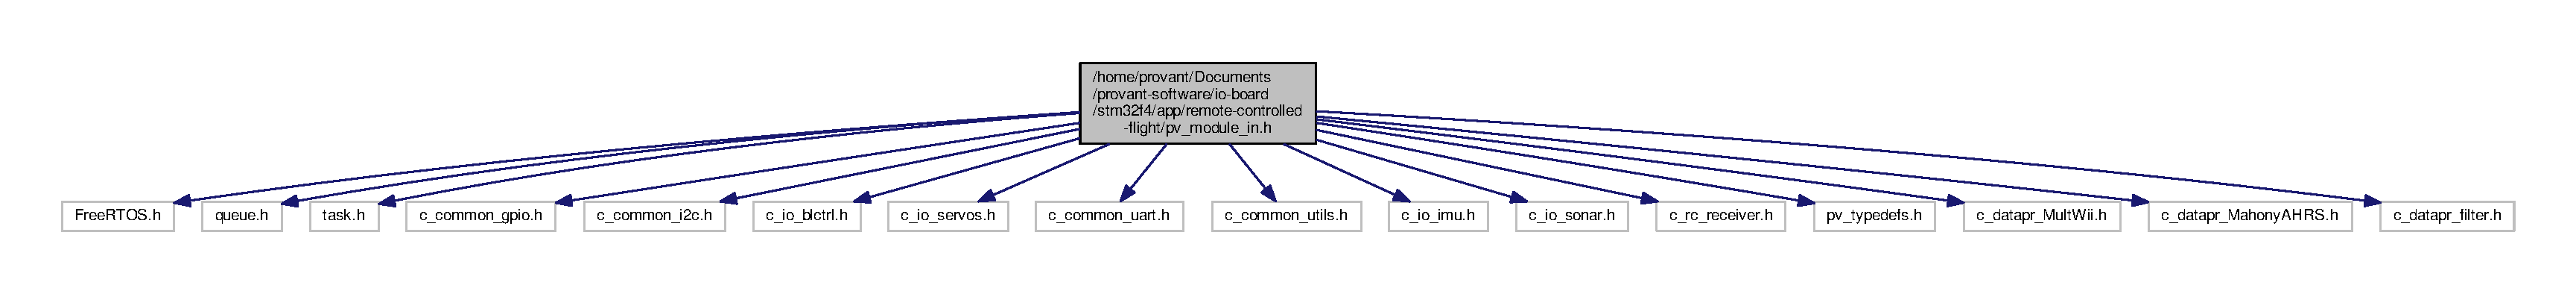
\includegraphics[width=350pt]{pv__module__in_8h__incl}
\end{center}
\end{figure}
This graph shows which files directly or indirectly include this file\+:\nopagebreak
\begin{figure}[H]
\begin{center}
\leavevmode
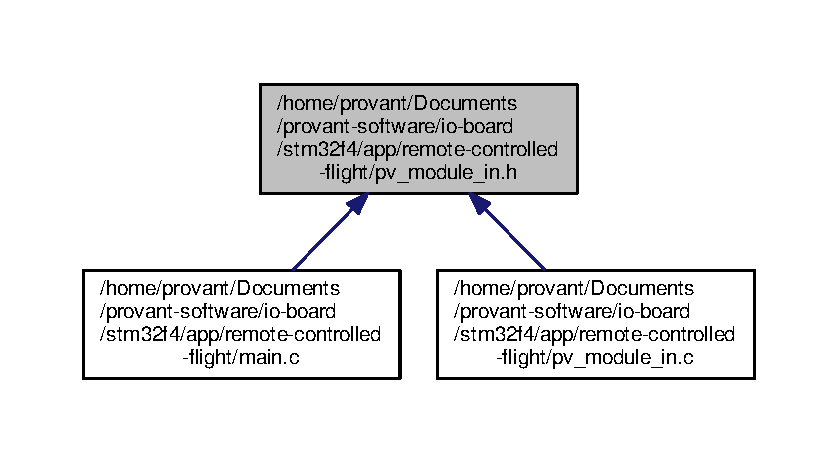
\includegraphics[width=350pt]{pv__module__in_8h__dep__incl}
\end{center}
\end{figure}
\subsection*{Data Structures}
\begin{DoxyCompactItemize}
\item 
struct \hyperlink{structpv__interface__in}{pv\+\_\+interface\+\_\+in}
\end{DoxyCompactItemize}
\subsection*{Macros}
\begin{DoxyCompactItemize}
\item 
\#define \hyperlink{pv__module__in_8h_a652f732918751d421cd00672fbcf34e6}{E\+N\+A\+B\+L\+E\+\_\+\+I\+MU}
\begin{DoxyCompactList}\small\item\em Define que modulos serao utilizados. \end{DoxyCompactList}\item 
\#define \hyperlink{pv__module__in_8h_ad825ce45a05b0e80e8d97f8cebd1ee76}{E\+N\+A\+B\+L\+E\+\_\+\+S\+E\+R\+VO}
\item 
\#define \hyperlink{pv__module__in_8h_a2856395932810f0a84e0e5f8efe14720}{E\+N\+A\+B\+L\+E\+\_\+\+A\+L\+T\+U\+RA}
\item 
\#define \hyperlink{pv__module__in_8h_acd356bc5fafb6cf72fd434275f0026a6}{E\+N\+A\+L\+B\+E\+\_\+\+D\+E\+B\+UG}
\item 
\#define \hyperlink{pv__module__in_8h_aa357c745fd8342c0d3837614e8f66f58}{A\+T\+T\+I\+T\+U\+D\+E\+\_\+\+M\+I\+N\+I\+M\+U\+M\+\_\+\+S\+T\+EP}~0.\+01
\item 
\#define \hyperlink{pv__module__in_8h_ae4ea5b3f1cbc2d035c41b6109eed0be7}{L\+I\+M\+I\+T\+\_\+\+S\+O\+N\+A\+R\+\_\+\+V\+AR}
\item 
\#define \hyperlink{pv__module__in_8h_a488238590df7f864862ba53318248c21}{S\+O\+N\+A\+R\+\_\+\+M\+A\+X\+\_\+\+V\+AR}~0.\+5
\item 
\#define \hyperlink{pv__module__in_8h_ac222db61ccc923f24415d8085bef26df}{D\+SB}~0.\+21
\item 
\#define \hyperlink{pv__module__in_8h_a36e061088806ff253cf7c99acdd12a0a}{S\+O\+N\+A\+R\+\_\+\+F\+I\+L\+T\+E\+R\+\_\+1\+\_\+\+O\+R\+D\+E\+R\+\_\+10\+HZ}
\item 
\#define \hyperlink{pv__module__in_8h_ada7264418a41278b0690fb70277a2ffa}{I\+N\+I\+T\+\_\+\+I\+T\+E\+R\+A\+T\+I\+O\+NS}~1000
\end{DoxyCompactItemize}
\subsection*{Functions}
\begin{DoxyCompactItemize}
\item 
void \hyperlink{group__app__in_gaffe0980a750cbec13ebf241c933460dd}{module\+\_\+in\+\_\+init} ()
\begin{DoxyCompactList}\small\item\em Inicializacao componentes de IO. \end{DoxyCompactList}\item 
void \hyperlink{group__app__in_ga2b56089e4c5adb9ac8b7a41fc1a0b0b2}{module\+\_\+in\+\_\+run} ()
\begin{DoxyCompactList}\small\item\em Função principal do módulo de IO. \end{DoxyCompactList}\end{DoxyCompactItemize}
\subsection*{Variables}
\begin{DoxyCompactItemize}
\item 
struct \hyperlink{structpv__interface__in}{pv\+\_\+interface\+\_\+in} \hyperlink{pv__module__in_8h_adb91b9002b5ee35e4d9c1b0a1eb2b6e3}{pv\+\_\+interface\+\_\+in}
\end{DoxyCompactItemize}


\subsection{Macro Definition Documentation}
\index{pv\+\_\+module\+\_\+in.\+h@{pv\+\_\+module\+\_\+in.\+h}!A\+T\+T\+I\+T\+U\+D\+E\+\_\+\+M\+I\+N\+I\+M\+U\+M\+\_\+\+S\+T\+EP@{A\+T\+T\+I\+T\+U\+D\+E\+\_\+\+M\+I\+N\+I\+M\+U\+M\+\_\+\+S\+T\+EP}}
\index{A\+T\+T\+I\+T\+U\+D\+E\+\_\+\+M\+I\+N\+I\+M\+U\+M\+\_\+\+S\+T\+EP@{A\+T\+T\+I\+T\+U\+D\+E\+\_\+\+M\+I\+N\+I\+M\+U\+M\+\_\+\+S\+T\+EP}!pv\+\_\+module\+\_\+in.\+h@{pv\+\_\+module\+\_\+in.\+h}}
\subsubsection[{\texorpdfstring{A\+T\+T\+I\+T\+U\+D\+E\+\_\+\+M\+I\+N\+I\+M\+U\+M\+\_\+\+S\+T\+EP}{ATTITUDE_MINIMUM_STEP}}]{\setlength{\rightskip}{0pt plus 5cm}\#define A\+T\+T\+I\+T\+U\+D\+E\+\_\+\+M\+I\+N\+I\+M\+U\+M\+\_\+\+S\+T\+EP~0.\+01}\hypertarget{pv__module__in_8h_aa357c745fd8342c0d3837614e8f66f58}{}\label{pv__module__in_8h_aa357c745fd8342c0d3837614e8f66f58}


Definition at line 32 of file pv\+\_\+module\+\_\+in.\+h.

\index{pv\+\_\+module\+\_\+in.\+h@{pv\+\_\+module\+\_\+in.\+h}!D\+SB@{D\+SB}}
\index{D\+SB@{D\+SB}!pv\+\_\+module\+\_\+in.\+h@{pv\+\_\+module\+\_\+in.\+h}}
\subsubsection[{\texorpdfstring{D\+SB}{DSB}}]{\setlength{\rightskip}{0pt plus 5cm}\#define D\+SB~0.\+21}\hypertarget{pv__module__in_8h_ac222db61ccc923f24415d8085bef26df}{}\label{pv__module__in_8h_ac222db61ccc923f24415d8085bef26df}


Definition at line 42 of file pv\+\_\+module\+\_\+in.\+h.

\index{pv\+\_\+module\+\_\+in.\+h@{pv\+\_\+module\+\_\+in.\+h}!E\+N\+A\+B\+L\+E\+\_\+\+A\+L\+T\+U\+RA@{E\+N\+A\+B\+L\+E\+\_\+\+A\+L\+T\+U\+RA}}
\index{E\+N\+A\+B\+L\+E\+\_\+\+A\+L\+T\+U\+RA@{E\+N\+A\+B\+L\+E\+\_\+\+A\+L\+T\+U\+RA}!pv\+\_\+module\+\_\+in.\+h@{pv\+\_\+module\+\_\+in.\+h}}
\subsubsection[{\texorpdfstring{E\+N\+A\+B\+L\+E\+\_\+\+A\+L\+T\+U\+RA}{ENABLE_ALTURA}}]{\setlength{\rightskip}{0pt plus 5cm}\#define E\+N\+A\+B\+L\+E\+\_\+\+A\+L\+T\+U\+RA}\hypertarget{pv__module__in_8h_a2856395932810f0a84e0e5f8efe14720}{}\label{pv__module__in_8h_a2856395932810f0a84e0e5f8efe14720}


Definition at line 28 of file pv\+\_\+module\+\_\+in.\+h.

\index{pv\+\_\+module\+\_\+in.\+h@{pv\+\_\+module\+\_\+in.\+h}!E\+N\+A\+B\+L\+E\+\_\+\+I\+MU@{E\+N\+A\+B\+L\+E\+\_\+\+I\+MU}}
\index{E\+N\+A\+B\+L\+E\+\_\+\+I\+MU@{E\+N\+A\+B\+L\+E\+\_\+\+I\+MU}!pv\+\_\+module\+\_\+in.\+h@{pv\+\_\+module\+\_\+in.\+h}}
\subsubsection[{\texorpdfstring{E\+N\+A\+B\+L\+E\+\_\+\+I\+MU}{ENABLE_IMU}}]{\setlength{\rightskip}{0pt plus 5cm}\#define E\+N\+A\+B\+L\+E\+\_\+\+I\+MU}\hypertarget{pv__module__in_8h_a652f732918751d421cd00672fbcf34e6}{}\label{pv__module__in_8h_a652f732918751d421cd00672fbcf34e6}


Define que modulos serao utilizados. 

Se E\+N\+A\+B\+L\+E\+\_\+$\ast$ 1 então tal modulo será utilizado 

Definition at line 26 of file pv\+\_\+module\+\_\+in.\+h.

\index{pv\+\_\+module\+\_\+in.\+h@{pv\+\_\+module\+\_\+in.\+h}!E\+N\+A\+B\+L\+E\+\_\+\+S\+E\+R\+VO@{E\+N\+A\+B\+L\+E\+\_\+\+S\+E\+R\+VO}}
\index{E\+N\+A\+B\+L\+E\+\_\+\+S\+E\+R\+VO@{E\+N\+A\+B\+L\+E\+\_\+\+S\+E\+R\+VO}!pv\+\_\+module\+\_\+in.\+h@{pv\+\_\+module\+\_\+in.\+h}}
\subsubsection[{\texorpdfstring{E\+N\+A\+B\+L\+E\+\_\+\+S\+E\+R\+VO}{ENABLE_SERVO}}]{\setlength{\rightskip}{0pt plus 5cm}\#define E\+N\+A\+B\+L\+E\+\_\+\+S\+E\+R\+VO}\hypertarget{pv__module__in_8h_ad825ce45a05b0e80e8d97f8cebd1ee76}{}\label{pv__module__in_8h_ad825ce45a05b0e80e8d97f8cebd1ee76}


Definition at line 27 of file pv\+\_\+module\+\_\+in.\+h.

\index{pv\+\_\+module\+\_\+in.\+h@{pv\+\_\+module\+\_\+in.\+h}!E\+N\+A\+L\+B\+E\+\_\+\+D\+E\+B\+UG@{E\+N\+A\+L\+B\+E\+\_\+\+D\+E\+B\+UG}}
\index{E\+N\+A\+L\+B\+E\+\_\+\+D\+E\+B\+UG@{E\+N\+A\+L\+B\+E\+\_\+\+D\+E\+B\+UG}!pv\+\_\+module\+\_\+in.\+h@{pv\+\_\+module\+\_\+in.\+h}}
\subsubsection[{\texorpdfstring{E\+N\+A\+L\+B\+E\+\_\+\+D\+E\+B\+UG}{ENALBE_DEBUG}}]{\setlength{\rightskip}{0pt plus 5cm}\#define E\+N\+A\+L\+B\+E\+\_\+\+D\+E\+B\+UG}\hypertarget{pv__module__in_8h_acd356bc5fafb6cf72fd434275f0026a6}{}\label{pv__module__in_8h_acd356bc5fafb6cf72fd434275f0026a6}


Definition at line 29 of file pv\+\_\+module\+\_\+in.\+h.

\index{pv\+\_\+module\+\_\+in.\+h@{pv\+\_\+module\+\_\+in.\+h}!I\+N\+I\+T\+\_\+\+I\+T\+E\+R\+A\+T\+I\+O\+NS@{I\+N\+I\+T\+\_\+\+I\+T\+E\+R\+A\+T\+I\+O\+NS}}
\index{I\+N\+I\+T\+\_\+\+I\+T\+E\+R\+A\+T\+I\+O\+NS@{I\+N\+I\+T\+\_\+\+I\+T\+E\+R\+A\+T\+I\+O\+NS}!pv\+\_\+module\+\_\+in.\+h@{pv\+\_\+module\+\_\+in.\+h}}
\subsubsection[{\texorpdfstring{I\+N\+I\+T\+\_\+\+I\+T\+E\+R\+A\+T\+I\+O\+NS}{INIT_ITERATIONS}}]{\setlength{\rightskip}{0pt plus 5cm}\#define I\+N\+I\+T\+\_\+\+I\+T\+E\+R\+A\+T\+I\+O\+NS~1000}\hypertarget{pv__module__in_8h_ada7264418a41278b0690fb70277a2ffa}{}\label{pv__module__in_8h_ada7264418a41278b0690fb70277a2ffa}


Definition at line 49 of file pv\+\_\+module\+\_\+in.\+h.

\index{pv\+\_\+module\+\_\+in.\+h@{pv\+\_\+module\+\_\+in.\+h}!L\+I\+M\+I\+T\+\_\+\+S\+O\+N\+A\+R\+\_\+\+V\+AR@{L\+I\+M\+I\+T\+\_\+\+S\+O\+N\+A\+R\+\_\+\+V\+AR}}
\index{L\+I\+M\+I\+T\+\_\+\+S\+O\+N\+A\+R\+\_\+\+V\+AR@{L\+I\+M\+I\+T\+\_\+\+S\+O\+N\+A\+R\+\_\+\+V\+AR}!pv\+\_\+module\+\_\+in.\+h@{pv\+\_\+module\+\_\+in.\+h}}
\subsubsection[{\texorpdfstring{L\+I\+M\+I\+T\+\_\+\+S\+O\+N\+A\+R\+\_\+\+V\+AR}{LIMIT_SONAR_VAR}}]{\setlength{\rightskip}{0pt plus 5cm}\#define L\+I\+M\+I\+T\+\_\+\+S\+O\+N\+A\+R\+\_\+\+V\+AR}\hypertarget{pv__module__in_8h_ae4ea5b3f1cbc2d035c41b6109eed0be7}{}\label{pv__module__in_8h_ae4ea5b3f1cbc2d035c41b6109eed0be7}


Definition at line 40 of file pv\+\_\+module\+\_\+in.\+h.

\index{pv\+\_\+module\+\_\+in.\+h@{pv\+\_\+module\+\_\+in.\+h}!S\+O\+N\+A\+R\+\_\+\+F\+I\+L\+T\+E\+R\+\_\+1\+\_\+\+O\+R\+D\+E\+R\+\_\+10\+HZ@{S\+O\+N\+A\+R\+\_\+\+F\+I\+L\+T\+E\+R\+\_\+1\+\_\+\+O\+R\+D\+E\+R\+\_\+10\+HZ}}
\index{S\+O\+N\+A\+R\+\_\+\+F\+I\+L\+T\+E\+R\+\_\+1\+\_\+\+O\+R\+D\+E\+R\+\_\+10\+HZ@{S\+O\+N\+A\+R\+\_\+\+F\+I\+L\+T\+E\+R\+\_\+1\+\_\+\+O\+R\+D\+E\+R\+\_\+10\+HZ}!pv\+\_\+module\+\_\+in.\+h@{pv\+\_\+module\+\_\+in.\+h}}
\subsubsection[{\texorpdfstring{S\+O\+N\+A\+R\+\_\+\+F\+I\+L\+T\+E\+R\+\_\+1\+\_\+\+O\+R\+D\+E\+R\+\_\+10\+HZ}{SONAR_FILTER_1_ORDER_10HZ}}]{\setlength{\rightskip}{0pt plus 5cm}\#define S\+O\+N\+A\+R\+\_\+\+F\+I\+L\+T\+E\+R\+\_\+1\+\_\+\+O\+R\+D\+E\+R\+\_\+10\+HZ}\hypertarget{pv__module__in_8h_a36e061088806ff253cf7c99acdd12a0a}{}\label{pv__module__in_8h_a36e061088806ff253cf7c99acdd12a0a}


Definition at line 45 of file pv\+\_\+module\+\_\+in.\+h.

\index{pv\+\_\+module\+\_\+in.\+h@{pv\+\_\+module\+\_\+in.\+h}!S\+O\+N\+A\+R\+\_\+\+M\+A\+X\+\_\+\+V\+AR@{S\+O\+N\+A\+R\+\_\+\+M\+A\+X\+\_\+\+V\+AR}}
\index{S\+O\+N\+A\+R\+\_\+\+M\+A\+X\+\_\+\+V\+AR@{S\+O\+N\+A\+R\+\_\+\+M\+A\+X\+\_\+\+V\+AR}!pv\+\_\+module\+\_\+in.\+h@{pv\+\_\+module\+\_\+in.\+h}}
\subsubsection[{\texorpdfstring{S\+O\+N\+A\+R\+\_\+\+M\+A\+X\+\_\+\+V\+AR}{SONAR_MAX_VAR}}]{\setlength{\rightskip}{0pt plus 5cm}\#define S\+O\+N\+A\+R\+\_\+\+M\+A\+X\+\_\+\+V\+AR~0.\+5}\hypertarget{pv__module__in_8h_a488238590df7f864862ba53318248c21}{}\label{pv__module__in_8h_a488238590df7f864862ba53318248c21}


Definition at line 41 of file pv\+\_\+module\+\_\+in.\+h.



\subsection{Variable Documentation}
\index{pv\+\_\+module\+\_\+in.\+h@{pv\+\_\+module\+\_\+in.\+h}!pv\+\_\+interface\+\_\+in@{pv\+\_\+interface\+\_\+in}}
\index{pv\+\_\+interface\+\_\+in@{pv\+\_\+interface\+\_\+in}!pv\+\_\+module\+\_\+in.\+h@{pv\+\_\+module\+\_\+in.\+h}}
\subsubsection[{\texorpdfstring{pv\+\_\+interface\+\_\+in}{pv_interface_in}}]{\setlength{\rightskip}{0pt plus 5cm}struct {\bf pv\+\_\+interface\+\_\+in}  {\bf pv\+\_\+interface\+\_\+in}}\hypertarget{pv__module__in_8h_adb91b9002b5ee35e4d9c1b0a1eb2b6e3}{}\label{pv__module__in_8h_adb91b9002b5ee35e4d9c1b0a1eb2b6e3}

\hypertarget{pv__module__sm_8c}{}\section{/home/provant/\+Documents/provant-\/software/io-\/board/stm32f4/app/remote-\/controlled-\/flight/pv\+\_\+module\+\_\+sm.c File Reference}
\label{pv__module__sm_8c}\index{/home/provant/\+Documents/provant-\/software/io-\/board/stm32f4/app/remote-\/controlled-\/flight/pv\+\_\+module\+\_\+sm.\+c@{/home/provant/\+Documents/provant-\/software/io-\/board/stm32f4/app/remote-\/controlled-\/flight/pv\+\_\+module\+\_\+sm.\+c}}


Implementação do módulo da maquinas de estados do V\+A\+NT.  


{\ttfamily \#include \char`\"{}pv\+\_\+module\+\_\+sm.\+h\char`\"{}}\\*
Include dependency graph for pv\+\_\+module\+\_\+sm.\+c\+:\nopagebreak
\begin{figure}[H]
\begin{center}
\leavevmode
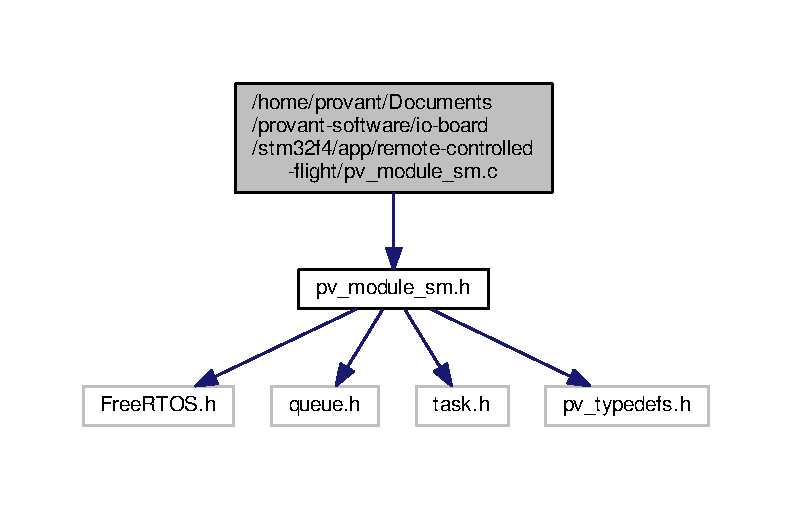
\includegraphics[width=350pt]{pv__module__sm_8c__incl}
\end{center}
\end{figure}
\subsection*{Macros}
\begin{DoxyCompactItemize}
\item 
\#define \hyperlink{group__app__sm_ga0ac6c9f2991b096e49c354e5cce6fae0}{M\+O\+D\+U\+L\+E\+\_\+\+P\+E\+R\+I\+OD}~20
\end{DoxyCompactItemize}
\subsection*{Functions}
\begin{DoxyCompactItemize}
\item 
void \hyperlink{group__app__sm_gaf1b95b5ff451c9c5d9a4cdd34531201b}{module\+\_\+sm\+\_\+init} ()
\begin{DoxyCompactList}\small\item\em Inicializacao do módulo de sm. \end{DoxyCompactList}\item 
void \hyperlink{group__app__sm_ga81e54a060d460608697719ba6afab1e4}{module\+\_\+sm\+\_\+run} ()
\begin{DoxyCompactList}\small\item\em Função principal do módulo da sm. \end{DoxyCompactList}\end{DoxyCompactItemize}
\subsection*{Variables}
\begin{DoxyCompactItemize}
\item 
port\+Tick\+Type \hyperlink{group__app__sm_gaa8db3871cb5f64abbd94ddd5a1db73a6}{last\+Wake\+Time}
\end{DoxyCompactItemize}


\subsection{Detailed Description}
Implementação do módulo da maquinas de estados do V\+A\+NT. 

\begin{DoxyAuthor}{Author}
Patrick Jose Pereira 
\end{DoxyAuthor}
\begin{DoxyVersion}{Version}
V1.\+0.\+0 
\end{DoxyVersion}
\begin{DoxyDate}{Date}
27-\/\+August-\/2014 
\end{DoxyDate}

\hypertarget{pv__module__sm_8h}{}\section{/home/provant/\+Documents/provant-\/software/io-\/board/stm32f4/app/remote-\/controlled-\/flight/pv\+\_\+module\+\_\+sm.h File Reference}
\label{pv__module__sm_8h}\index{/home/provant/\+Documents/provant-\/software/io-\/board/stm32f4/app/remote-\/controlled-\/flight/pv\+\_\+module\+\_\+sm.\+h@{/home/provant/\+Documents/provant-\/software/io-\/board/stm32f4/app/remote-\/controlled-\/flight/pv\+\_\+module\+\_\+sm.\+h}}


Implementação do módulo da maquinas de estados do V\+A\+NT.  


{\ttfamily \#include \char`\"{}Free\+R\+T\+O\+S.\+h\char`\"{}}\\*
{\ttfamily \#include \char`\"{}queue.\+h\char`\"{}}\\*
{\ttfamily \#include \char`\"{}task.\+h\char`\"{}}\\*
{\ttfamily \#include \char`\"{}pv\+\_\+typedefs.\+h\char`\"{}}\\*
Include dependency graph for pv\+\_\+module\+\_\+sm.\+h\+:\nopagebreak
\begin{figure}[H]
\begin{center}
\leavevmode
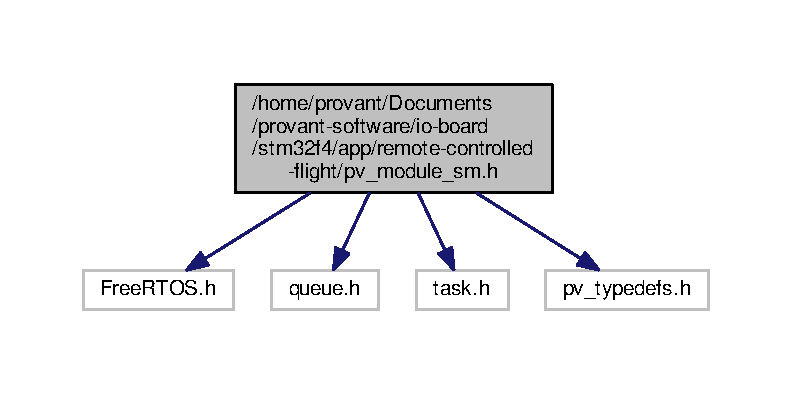
\includegraphics[width=350pt]{pv__module__sm_8h__incl}
\end{center}
\end{figure}
This graph shows which files directly or indirectly include this file\+:\nopagebreak
\begin{figure}[H]
\begin{center}
\leavevmode
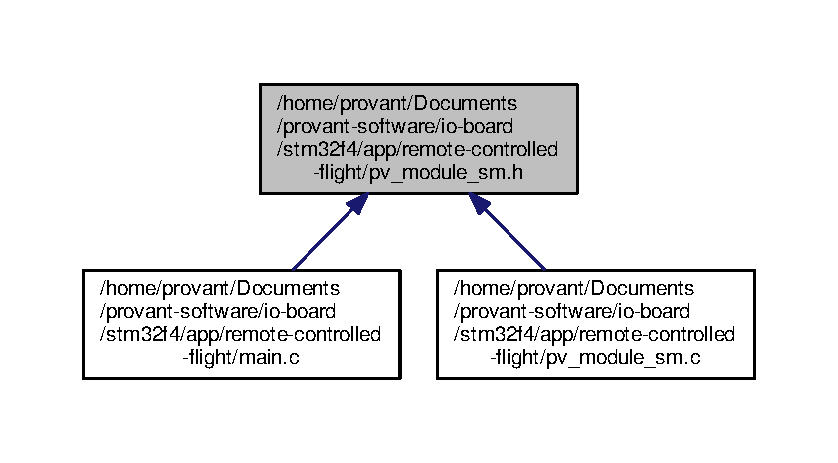
\includegraphics[width=350pt]{pv__module__sm_8h__dep__incl}
\end{center}
\end{figure}
\subsection*{Functions}
\begin{DoxyCompactItemize}
\item 
void \hyperlink{group__app__sm_gaf1b95b5ff451c9c5d9a4cdd34531201b}{module\+\_\+sm\+\_\+init} ()
\begin{DoxyCompactList}\small\item\em Inicializacao do módulo de sm. \end{DoxyCompactList}\item 
void \hyperlink{group__app__sm_ga81e54a060d460608697719ba6afab1e4}{module\+\_\+sm\+\_\+run} ()
\begin{DoxyCompactList}\small\item\em Função principal do módulo da sm. \end{DoxyCompactList}\end{DoxyCompactItemize}


\subsection{Detailed Description}
Implementação do módulo da maquinas de estados do V\+A\+NT. 

\begin{DoxyAuthor}{Author}
Patrick Jose Pereira 
\end{DoxyAuthor}
\begin{DoxyVersion}{Version}
V1.\+0.\+0 
\end{DoxyVersion}
\begin{DoxyDate}{Date}
27-\/\+August-\/2014 
\end{DoxyDate}

%--- End generated contents ---

% Index
\backmatter
\newpage
\phantomsection
\clearemptydoublepage
\addcontentsline{toc}{chapter}{Index}
\printindex

\end{document}
